\documentclass[journal,12pt,twocolumn]{IEEEtran}
%
\usepackage{setspace}
\usepackage{gensymb}
%\doublespacing
\singlespacing

%\usepackage{graphicx}
%\usepackage{amssymb}
%\usepackage{relsize}
\usepackage[cmex10]{amsmath}
%\usepackage{amsthm}
%\interdisplaylinepenalty=2500
%\savesymbol{iint}
%\usepackage{txfonts}
%\restoresymbol{TXF}{iint}
%\usepackage{wasysym}
\usepackage{amsthm}
%\usepackage{iithtlc}
\usepackage{mathrsfs}
\usepackage{txfonts}
\usepackage{stfloats}
\usepackage{bm}
\usepackage{cite}
\usepackage{cases}
\usepackage{subfig}
%\usepackage{xtab}
\usepackage{longtable}
\usepackage{multirow}
%\usepackage{algorithm}
%\usepackage{algpseudocode}
\usepackage{enumitem}
\usepackage{mathtools}
\usepackage{tikz}
\usepackage{circuitikz}
\usepackage{verbatim}
\usepackage{tfrupee}
\usepackage[breaklinks=true]{hyperref}
%\usepackage{stmaryrd}
\usepackage{tkz-euclide} % loads  TikZ and tkz-base
\usetkzobj{all}
\usepackage{listings}
    \usepackage{color}                                            %%
    \usepackage{array}                                            %%
    \usepackage{longtable}                                        %%
    \usepackage{calc}                                             %%
    \usepackage{multirow}                                         %%
    \usepackage{hhline}                                           %%
    \usepackage{ifthen}                                           %%
  %optionally (for landscape tables embedded in another document): %%
    \usepackage{lscape}     
\usepackage{multicol}
\usepackage{chngcntr}
%\usepackage{enumerate}

%\usepackage{wasysym}
%\newcounter{MYtempeqncnt}
\DeclareMathOperator*{\Res}{Res}
%\renewcommand{\baselinestretch}{2}
\renewcommand\thesection{\arabic{section}}
\renewcommand\thesubsection{\thesection.\arabic{subsection}}
\renewcommand\thesubsubsection{\thesubsection.\arabic{subsubsection}}

\renewcommand\thesectiondis{\arabic{section}}
\renewcommand\thesubsectiondis{\thesectiondis.\arabic{subsection}}
\renewcommand\thesubsubsectiondis{\thesubsectiondis.\arabic{subsubsection}}

% correct bad hyphenation here
\hyphenation{op-tical net-works semi-conduc-tor}
\def\inputGnumericTable{}                                 %%

\lstset{
%language=C,
frame=single, 
breaklines=true,
columns=fullflexible
}
%\lstset{
%language=tex,
%frame=single, 
%breaklines=true
%}

\begin{document}
%


\newtheorem{theorem}{Theorem}[section]
\newtheorem{problem}{Problem}
\newtheorem{proposition}{Proposition}[section]
\newtheorem{lemma}{Lemma}[section]
\newtheorem{corollary}[theorem]{Corollary}
\newtheorem{example}{Example}[section]
\newtheorem{definition}[problem]{Definition}
%\newtheorem{thm}{Theorem}[section] 
%\newtheorem{defn}[thm]{Definition}
%\newtheorem{algorithm}{Algorithm}[section]
%\newtheorem{cor}{Corollary}
\newcommand{\BEQA}{\begin{eqnarray}}
\newcommand{\EEQA}{\end{eqnarray}}
\newcommand{\define}{\stackrel{\triangle}{=}}

\bibliographystyle{IEEEtran}
%\bibliographystyle{ieeetr}


\providecommand{\mbf}{\mathbf}
\providecommand{\pr}[1]{\ensuremath{\Pr\left(#1\right)}}
\providecommand{\qfunc}[1]{\ensuremath{Q\left(#1\right)}}
\providecommand{\sbrak}[1]{\ensuremath{{}\left[#1\right]}}
\providecommand{\lsbrak}[1]{\ensuremath{{}\left[#1\right.}}
\providecommand{\rsbrak}[1]{\ensuremath{{}\left.#1\right]}}
\providecommand{\brak}[1]{\ensuremath{\left(#1\right)}}
\providecommand{\lbrak}[1]{\ensuremath{\left(#1\right.}}
\providecommand{\rbrak}[1]{\ensuremath{\left.#1\right)}}
\providecommand{\cbrak}[1]{\ensuremath{\left\{#1\right\}}}
\providecommand{\lcbrak}[1]{\ensuremath{\left\{#1\right.}}
\providecommand{\rcbrak}[1]{\ensuremath{\left.#1\right\}}}
\theoremstyle{remark}
\newtheorem{rem}{Remark}
\newcommand{\sgn}{\mathop{\mathrm{sgn}}}
\providecommand{\abs}[1]{\left\vert#1\right\vert}
\providecommand{\res}[1]{\Res\displaylimits_{#1}} 
\providecommand{\norm}[1]{\left\lVert#1\right\rVert}
%\providecommand{\norm}[1]{\lVert#1\rVert}
\providecommand{\mtx}[1]{\mathbf{#1}}
\providecommand{\mean}[1]{E\left[ #1 \right]}
\providecommand{\fourier}{\overset{\mathcal{F}}{ \rightleftharpoons}}
%\providecommand{\hilbert}{\overset{\mathcal{H}}{ \rightleftharpoons}}
\providecommand{\system}{\overset{\mathcal{H}}{ \longleftrightarrow}}
	%\newcommand{\solution}[2]{\textbf{Solution:}{#1}}
\newcommand{\solution}{\noindent \textbf{Solution: }}
\newcommand{\cosec}{\,\text{cosec}\,}
\providecommand{\dec}[2]{\ensuremath{\overset{#1}{\underset{#2}{\gtrless}}}}
\newcommand{\myvec}[1]{\ensuremath{\begin{pmatrix}#1\end{pmatrix}}}
\newcommand{\mydet}[1]{\ensuremath{\begin{vmatrix}#1\end{vmatrix}}}
%\numberwithin{equation}{section}
%\numberwithin{equation}{subsection}
%\numberwithin{problem}{section}
%\numberwithin{definition}{section}
\makeatletter
\@addtoreset{figure}{problem}
\makeatother

\let\StandardTheFigure\thefigure
\let\vec\mathbf
%\renewcommand{\thefigure}{\theproblem.\arabic{figure}}
\renewcommand{\thefigure}{\theproblem}
%\setlist[enumerate,1]{before=\renewcommand\theequation{\theenumi.\arabic{equation}}
%\counterwithin{equation}{enumi}


%\renewcommand{\theequation}{\arabic{subsection}.\arabic{equation}}

\def\putbox#1#2#3{\makebox[0in][l]{\makebox[#1][l]{}\raisebox{\baselineskip}[0in][0in]{\raisebox{#2}[0in][0in]{#3}}}}
     \def\rightbox#1{\makebox[0in][r]{#1}}
     \def\centbox#1{\makebox[0in]{#1}}
     \def\topbox#1{\raisebox{-\baselineskip}[0in][0in]{#1}}
     \def\midbox#1{\raisebox{-0.5\baselineskip}[0in][0in]{#1}}

\vspace{3cm}

\title{
	\logo{
EE2227 Control System Documentation.
	}
}
\author{ G V V Sharma$^{*}$% <-this % stops a space
	\thanks{*The author is with the Department
		of Electrical Engineering, Indian Institute of Technology, Hyderabad
		502285 India e-mail:  gadepall@iith.ac.in. All content in this manual is released under GNU GPL.  Free and open source.}
	
}	
%\title{
%	\logo{Matrix Analysis through Octave}{\begin{center}\includegraphics[scale=.24]{tlc}\end{center}}{}{HAMDSP}
%}


% paper title
% can use linebreaks \\ within to get better formatting as desired
%\title{Matrix Analysis through Octave}
%
%
% author names and IEEE memberships
% note positions of commas and nonbreaking spaces ( ~ ) LaTeX will not break
% a structure at a ~ so this keeps an author's name from being broken across
% two lines.
% use \thanks{} to gain access to the first footnote area
% a separate \thanks must be used for each paragraph as LaTeX2e's \thanks
% was not built to handle multiple paragraphs
%

%\author{<-this % stops a space
%\thanks{}}
%}
% note the % following the last \IEEEmembership and also \thanks - 
% these prevent an unwanted space from occurring between the last author name
% and the end of the author line. i.e., if you had this:
% 
% \author{....lastname \thanks{...} \thanks{...} }
%                     ^------------^------------^----Do not want these spaces!
%
% a space would be appended to the last name and could cause every name on that
% line to be shifted left slightly. This is one of those "LaTeX things". For
% instance, "\textbf{A} \textbf{B}" will typeset as "A B" not "AB". To get
% "AB" then you have to do: "\textbf{A}\textbf{B}"
% \thanks is no different in this regard, so shield the last } of each \thanks
% that ends a line with a % and do not let a space in before the next \thanks.
% Spaces after \IEEEmembership other than the last one are OK (and needed) as
% you are supposed to have spaces between the names. For what it is worth,
% this is a minor point as most people would not even notice if the said evil
% space somehow managed to creep in.



% The paper headers
%\markboth{Journal of \LaTeX\ Class Files,~Vol.~6, No.~1, January~2007}%
%{Shell \MakeLowercase{\textit{et al.}}: Bare Demo of IEEEtran.cls for Journals}
% The only time the second header will appear is for the odd numbered pages
% after the title page when using the twoside option.
% 
% *** Note that you probably will NOT want to include the author's ***
% *** name in the headers of peer review papers.                   ***
% You can use \ifCLASSOPTIONpeerreview for conditional compilation here if
% you desire.




% If you want to put a publisher's ID mark on the page you can do it like
% this:
%\IEEEpubid{0000--0000/00\$00.00~\copyright~2007 IEEE}
% Remember, if you use this you must call \IEEEpubidadjcol in the second
% column for its text to clear the IEEEpubid mark.



% make the title area
\maketitle

\newpage

%\tableofcontents

\bigskip

\renewcommand{\thefigure}{\theenumi}
\renewcommand{\thetable}{\theenumi}
%\renewcommand{\theequation}{\theenumi}

%\begin{abstract}
%%\boldmath
%In this letter, an algorithm for evaluating the exact analytical bit error rate  (BER)  for the piecewise linear (PL) combiner for  multiple relays is presented. Previous results were available only for upto three relays. The algorithm is unique in the sense that  the actual mathematical expressions, that are prohibitively large, need not be explicitly obtained. The diversity gain due to multiple relays is shown through plots of the analytical BER, well supported by simulations. 
%
%\end{abstract}
% IEEEtran.cls defaults to using nonbold math in the Abstract.
% This preserves the distinction between vectors and scalars. However,
% if the journal you are submitting to favors bold math in the abstract,
% then you can use LaTeX's standard command \boldmath at the very start
% of the abstract to achieve this. Many IEEE journals frown on math
% in the abstract anyway.

% Note that keywords are not normally used for peerreview papers.
%\begin{IEEEkeywords}
%Cooperative diversity, decode and forward, piecewise linear
%\end{IEEEkeywords}



% For peer review papers, you can put extra information on the cover
% page as needed:
% \ifCLASSOPTIONpeerreview
% \begin{center} \bfseries EDICS Category: 3-BBND \end{center}
% \fi
%
% For peerreview papers, this IEEEtran command inserts a page break and
% creates the second title. It will be ignored for other modes.
%\IEEEpeerreviewmaketitle

\begin{abstract}
Gate Control System Question and Solution 
%book provides an introduction to optimization  based on the NCERT textbooks from Class 6-12.  Links to sample Python codes are available in the text.  
\end{abstract}
\begin{frame}{Question-1}
%\begin{flushleft}
\textsf{ For an LTI system, the Bode plot for its gain is as illustrated in the figure shown. The number of system poles $N_{p}$ and number of system zeros $N_{z}$ in the frequency range 1 Hz $\leq$ f $\leq$ $10^{7}$ Hz is}
%\end{flushleft}

\begin{figure}[htp]
    \centering
    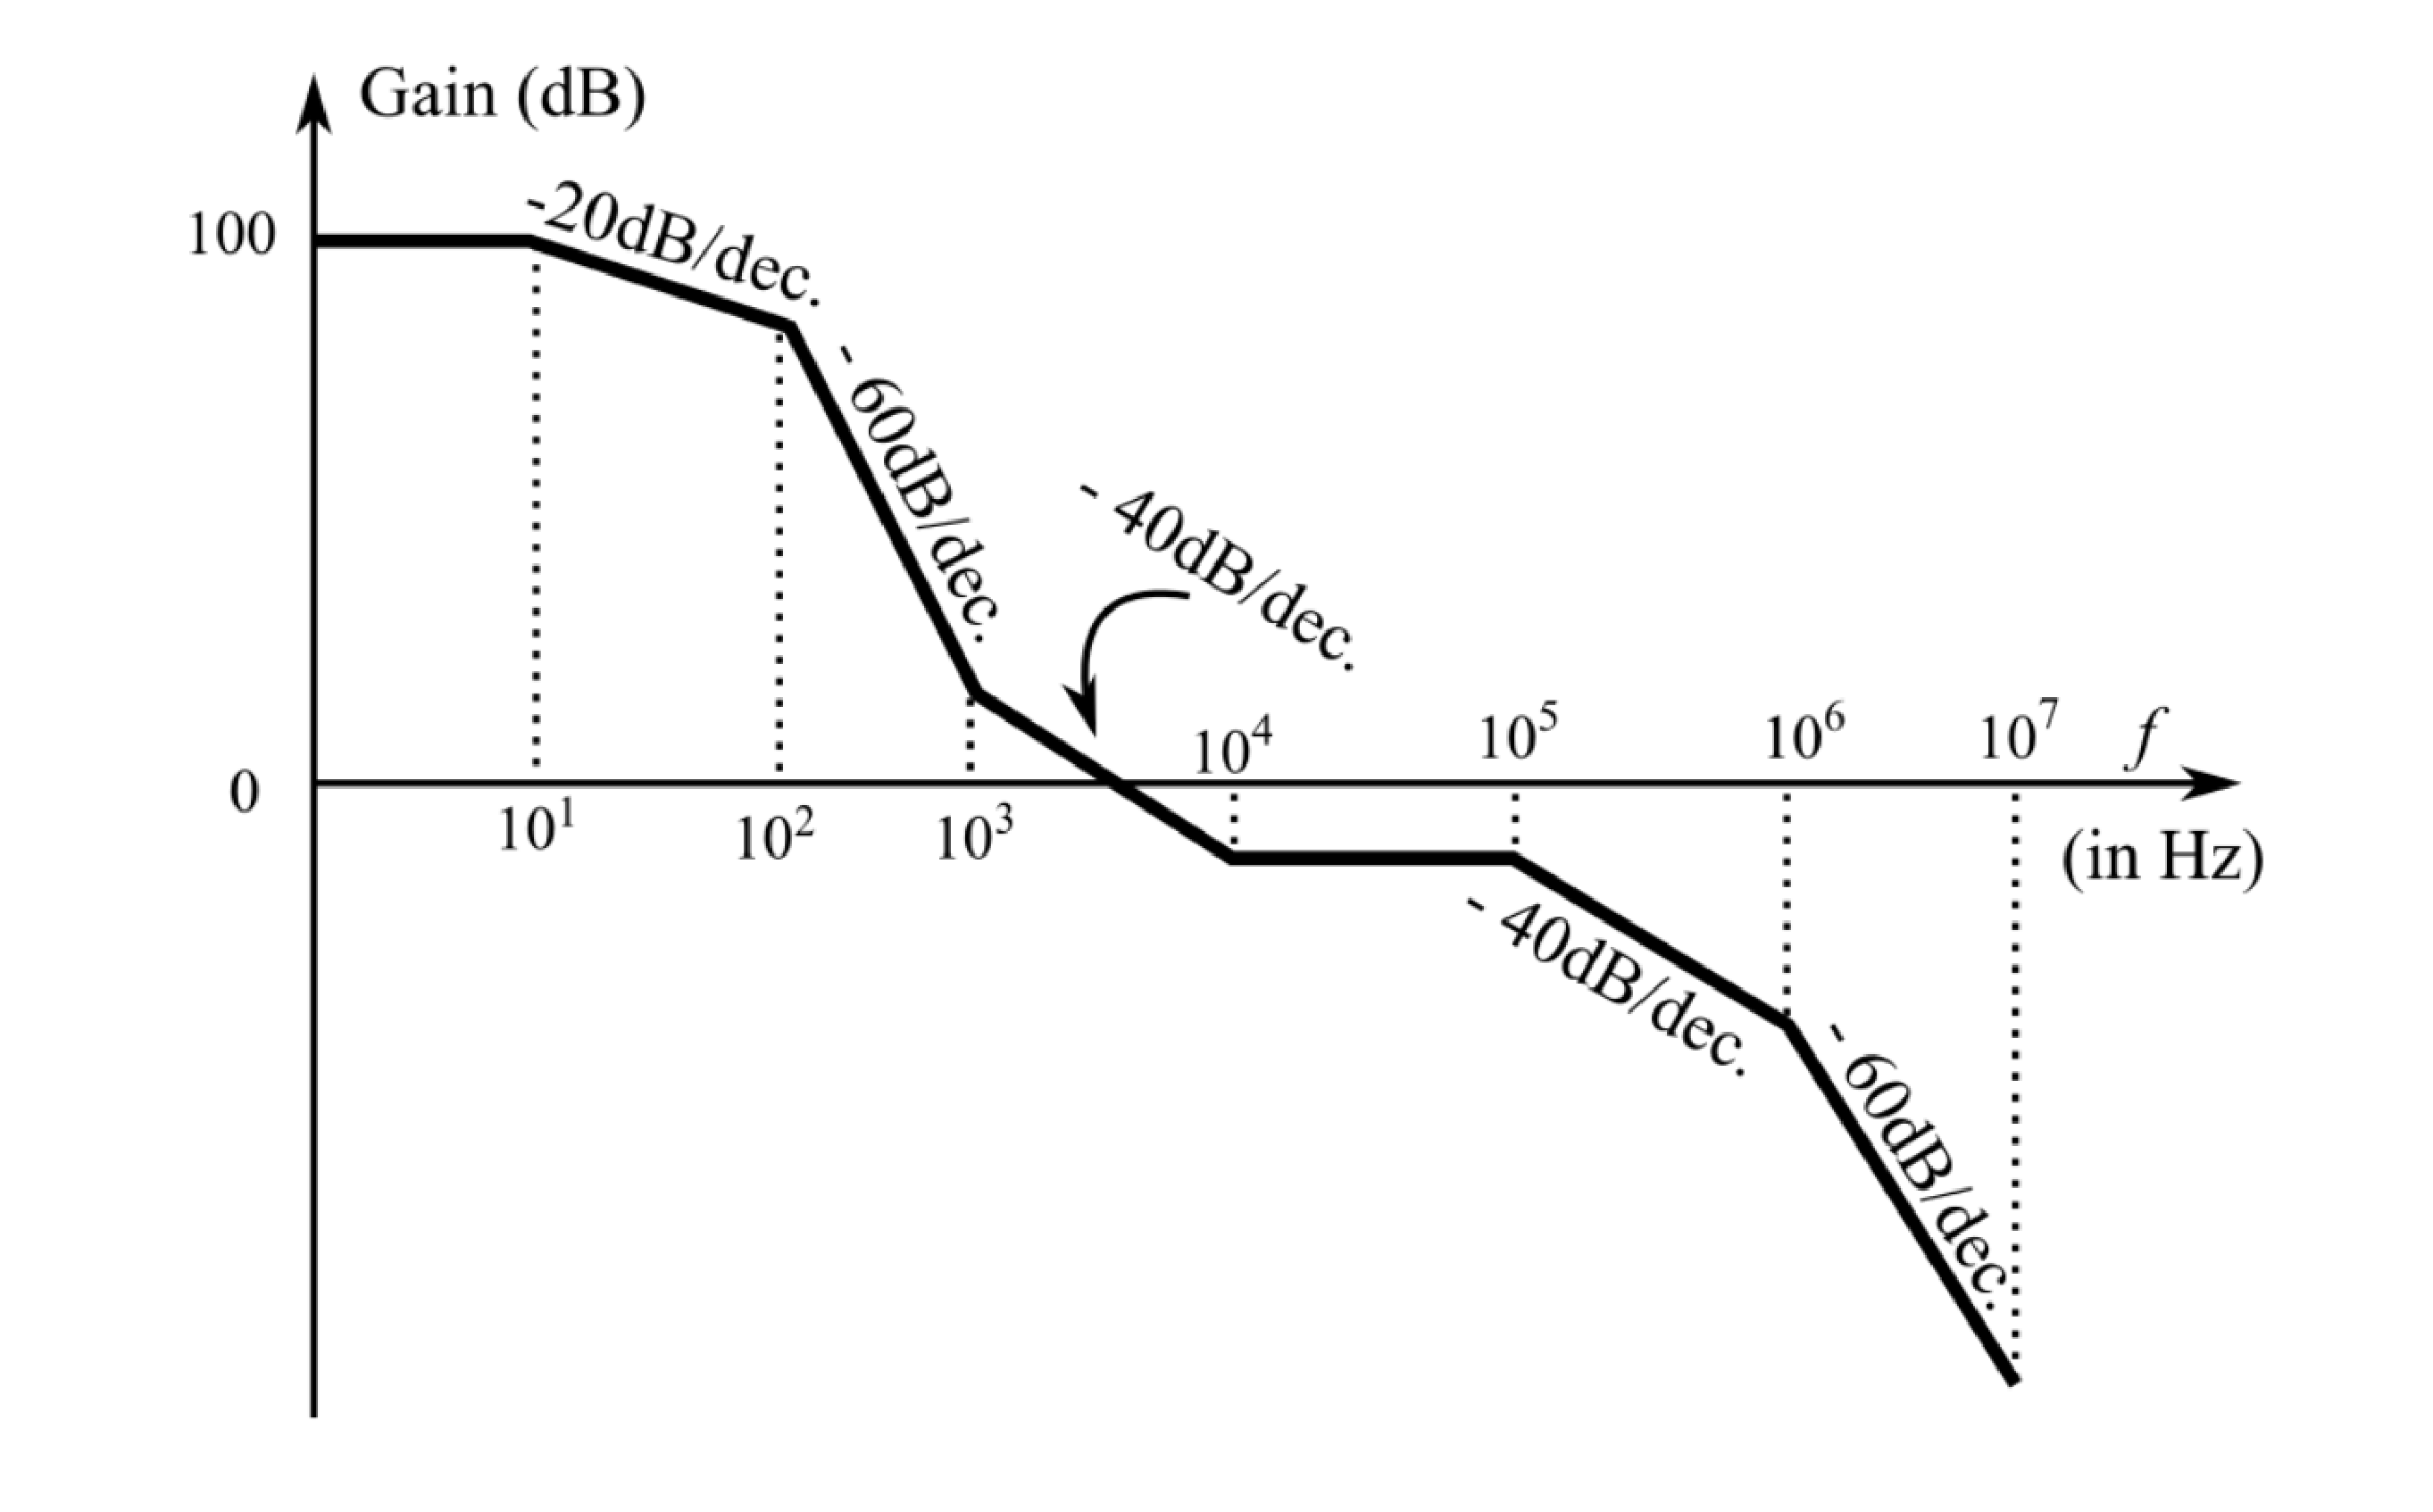
\includegraphics[width=9cm]{./figs/figure.eps}
    
    \label{fig:galaxy}
\end{figure}
\end{frame}
\begin{frame}{ Solution:- }
\begin{flushleft}
\textsf{Let us consider a generalized transfer gain}
\end{flushleft}
\vspace{10pt}
$H(s) = k \frac{(s-z_{1})(s-z_{2})...(s-z_{m-1})(s-z_{m})}{(s-p_{1})(s-p_{2})....(s-p_{n-1})(s-p_{n})}$\vspace{18pt}\\
$Gain = 20log|H(s)| = 20log|k| + 20log|s-z_{1}| + 20log|s-z_{2}| + ...... + 20log|s-z_{m}| - 20log|s-p_{1}| - 20log|s-p_{2}| - ..... - 20log|s-p_{n}| $ \vspace{18pt}

\begin{itemize}
    \item  When a pole is encountered the slope always decreases by -20 dB/decade
    \item When a zero is encountered the slope always increases by +20 dB/decade
\end{itemize}
\begin{itemize}
    \item At f = 10 Hz , change in slope = -20dB/sec, Hence we have 1 pole here
    \item At f = $10^{2}$ Hz, Change in slope = -40dB/sec, Hence we have 2 poles here
    
    
    
\end{itemize}

\begin{itemize}
\item At f = $10^{3}$ Hz, Change in slope = +20dB/sec, Hence we have 1 zero here
\item At f = $10^{4}$ Hz, Change in slope = +40dB/sec, Hence we have 2 zeros here

    
\end{itemize}


\end{frame}
\begin{itemize}

    \item At f = $10^{5}$ Hz, Change in slope = -40dB/sec, Hence we have 2 poles here
    \item At f = $10^{6}$ Hz, Change in slope = -20dB/sec, Hence we have 1 pole here
    
\end{itemize}
\end{frame}
$N_{p} = 6$  & 
$N_{z} = 3$ 
\\\\
\begin{frame}{Question-2}
Consider the following second order system with the transfer function:
$$G(s) = \frac{1}{1+2s+s^2}$$
\\with input unit step $$R(s) = \frac{1}{s}$$  Let C(s) be the corresponding output. The time taken by the system output c(t) to reach 94\% of its steady state value, rounded off to two decimal places is
\medskip
\\ \hspace{20}(A)5.25\hspace{20}(B)4.50 \hspace{20}(C)3.89  \hspace{20}(D)2.81


\end{frame}
\begin{frame}{Solution:- }
The approach for finding the solution is as follows:
\begin{itemize}
    \item finding C(s)
    \item finding c(t)
    \item finding the time at which c(t) attains 94\% of its steady state value
\end{itemize}
\end{frame}
We are given G(s) and R(s), to find C(s), we can simply multiply these two
$$C(s) = R(s).G(s) = (\frac{1}{s})  (\frac{1}{1+2s+s^2})$$
$$C(s) =  \frac{1}{s(1+s)^2}
\end{frame}
To find c(t), we have to do inverse Laplace transform on C(s)
$$c(t) \longleftrightarrow C(s)$$
Inverse Laplace transform can be calculated by the formula:
$$f(t) = \frac{1}{2\pi j} \int_{a -j\infty}^{a+j\infty}F(s)e^{st} ds$$
From the above formula, the inverse Laplace for some common expressions are:
$$u(t) \longleftrightarrow \frac{1}{s}$$
$$e^{-at} u(t) \longleftrightarrow \frac{1}{s+a}$$
$$t e^{-at} u(t) \longleftrightarrow \frac{1}{(s+a)^2}$$

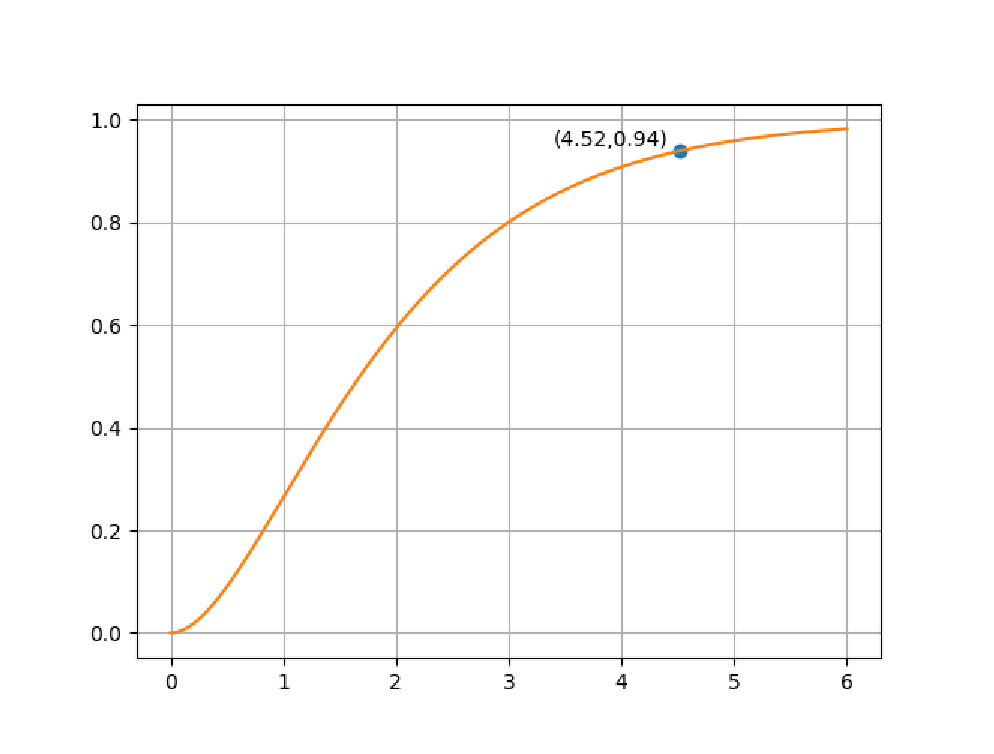
\includegraphics[scale=0.5]{./figs/plot.eps}

We found C(s) as:
$$C(s) =  \frac{1}{s(1+s)^2}$$
Now, we will use partial fractions to make applying Inverse Laplace easy.
$$C(s) =  \frac{1}{s(1+s)^2} =  \frac{A}{s} + \frac{B}{(1+s)} + \frac{C}{(1+s)^2}$$
We get, 
\begin{align*}
A &= 1 & A+B &=0 & 2A+B+C &= 0 \\
A &=1 & B &=-1 & C &=-1
\end{align*}
Therefore,
$$C(s) = \frac{1}{s} - \frac{1}{(1+s)} - \frac{1}{(1+s)^2}$$

$$c(t) = L^{-1} ( \frac{1}{s} - \frac{1}{(1+s)} - \frac{1}{(1+s)^2}) $$
From the properties of inverse Laplace transform,
$$L^{-1} (F_1(s) + F_2(s) + F_3(s)) = L^{-1}(F_1(s)) $$ 
$$ + L^{-1}(F_2(s)) + L^{-1}(F_3(s))$$
Therefore;
$$c(t) = L^{-1} ( \frac{1}{s}) - L^{-1}(\frac{1}{(1+s)}) - L^{-1}(\frac{1}{(1+s)^2}) $$
Using the Known inverse transforms:
$$c(t) = (1 - e^{-t} - te^{-t}) . u(t)$$

To know the steady state value of c(t), we calculate 
$$\lim_{t\to\infty} c(t) = (1+0+0).(1) = 1$$
Now, 94\% of 1 is 0.94, so we should now solve for a positive t such that
$$(1 - e^{-t} - te^{-t}) = 0.94$$
After calculation, t turns out to be
$$ t = 4.5221$$
Therefore, answer is option (b)
We can also find the solution by plotting c(t):
\\\\\

\begin{frame}{Question-3 }
The block diagram of a system is illustrated in the figure shown, where X(s) is the input and Y(s) is the output. The transfer function H(s)=$\frac{Y(s)}{X(s)}$ is 

(A) H(s)=$\frac{s^2+1}{s^3+s^2+s+1}$ \\
(B) H(s)=$\frac{s^2+1}{s^3+2s^2+s+1}$ \\
(C) H(s)=$\frac{s^2+1}{s^2+s+1}$ \\
(D) H(s)=$\frac{s^2+1}{2s^2+1}$
\end{frame}\\
\begin{figure}[h]
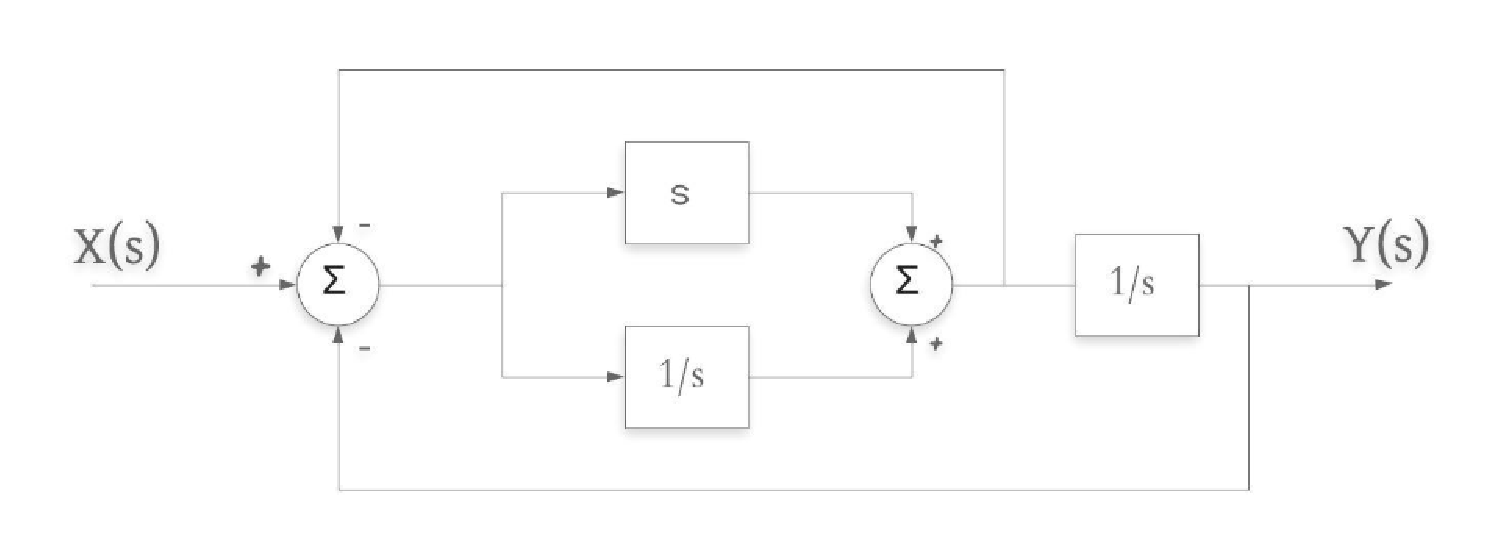
\includegraphics[width=0.5\textwidth]{./figs/pic1.eps}
\end{figure}

\\
\begin{frame}{Solution:- }
Here we have two transfer function s and $\frac{1}{s}$ in parallel with a adder as shown in figure.
After solving these two parallel transfer function by just adding both of them we will get
\begin{figure}[h]
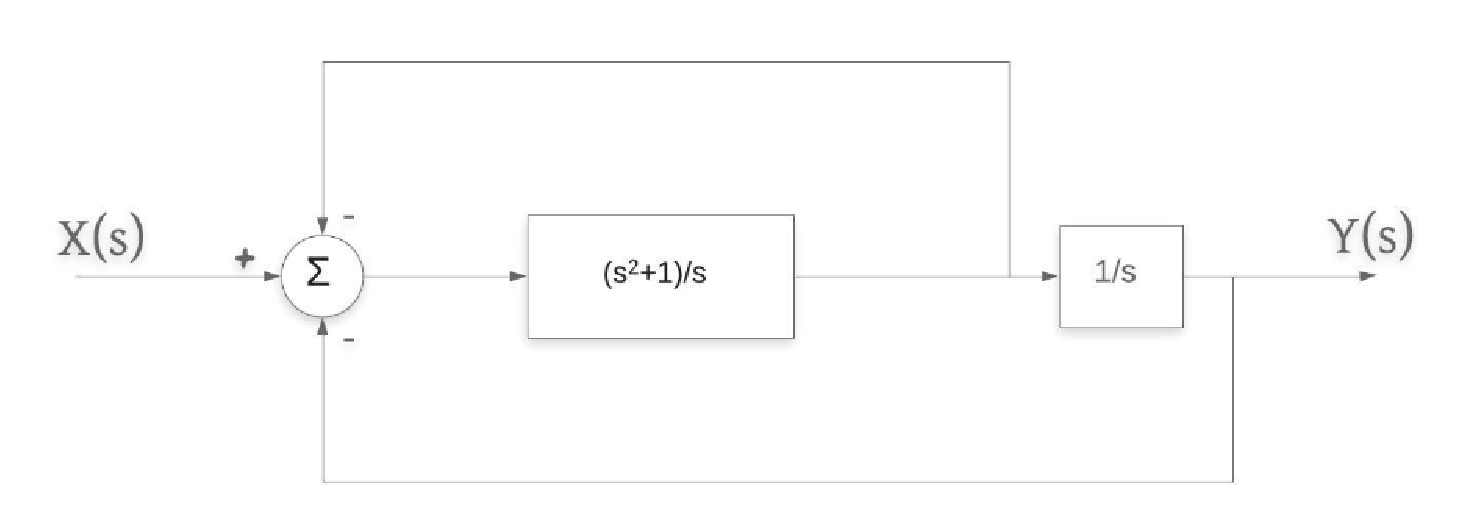
\includegraphics[width=0.5\textwidth]{./figs/pic2.eps}
\end{figure}
\\\\\\\\\\\
Now we will convert three input adder into two input adder as shown in figure given below.
\begin{figure}[h]
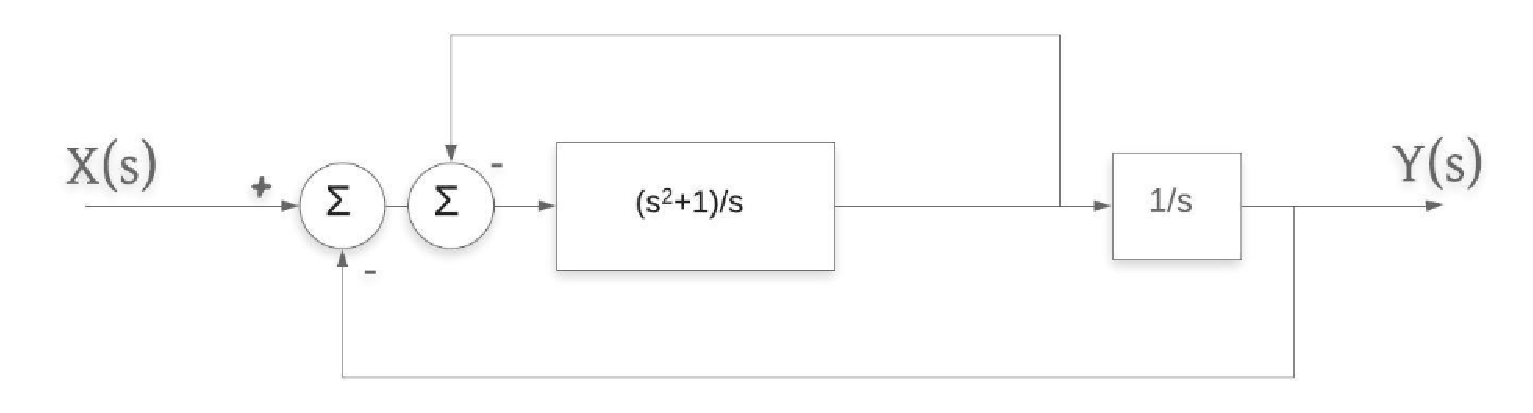
\includegraphics[width=0.5\textwidth]{./figs/pic3.eps}
\end{figure}
\\\\
Now we have Negative Unity Feedback System(NUFS) in closed loop transfer function. \\Let's say we have transfer function G(s) with Negative Unity Feedback System in closed loop then we will solve this by\\              $\frac{G(s)}{1+G(s)}$.
\\Here we have
\begin{figure}[h]
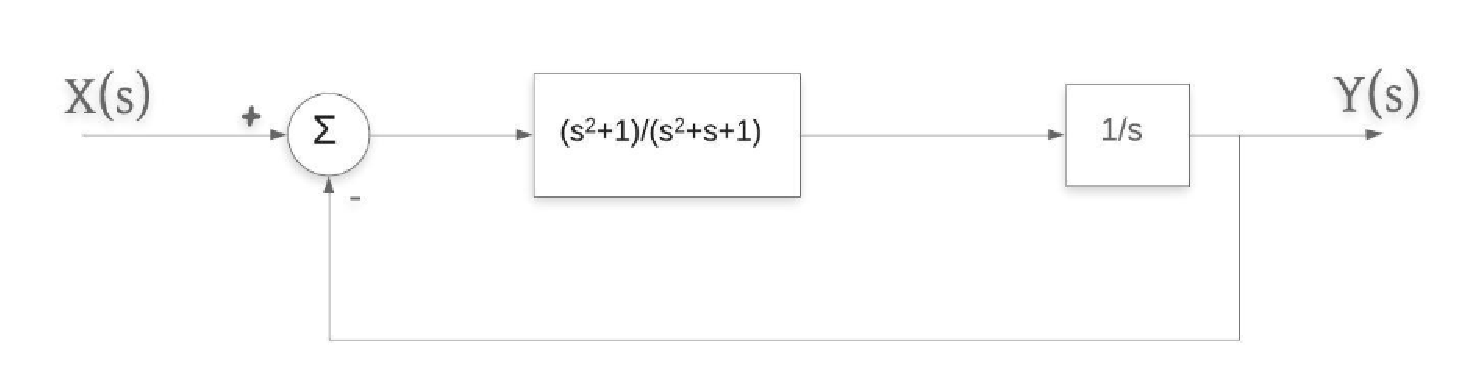
\includegraphics[width=0.5\textwidth]{./figs/pic4.eps}
\end{figure}
\\\
Here we have two transfer function in series 
\begin{figure}[h]
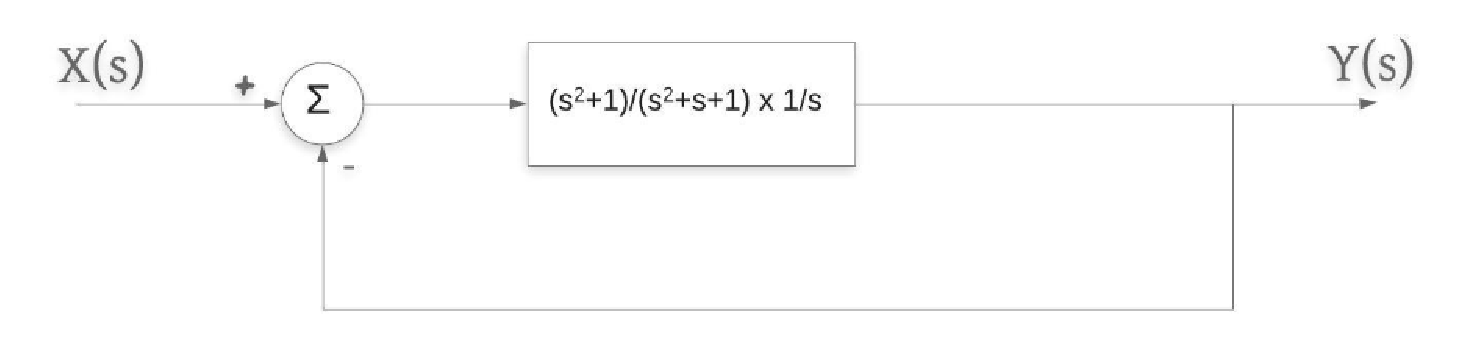
\includegraphics[width=0.5\textwidth]{./figs/pic5.eps}
\end{figure}
\\\\\\
Now we have one more transfer function with negative unity feedback.
\begin{figure}[h]
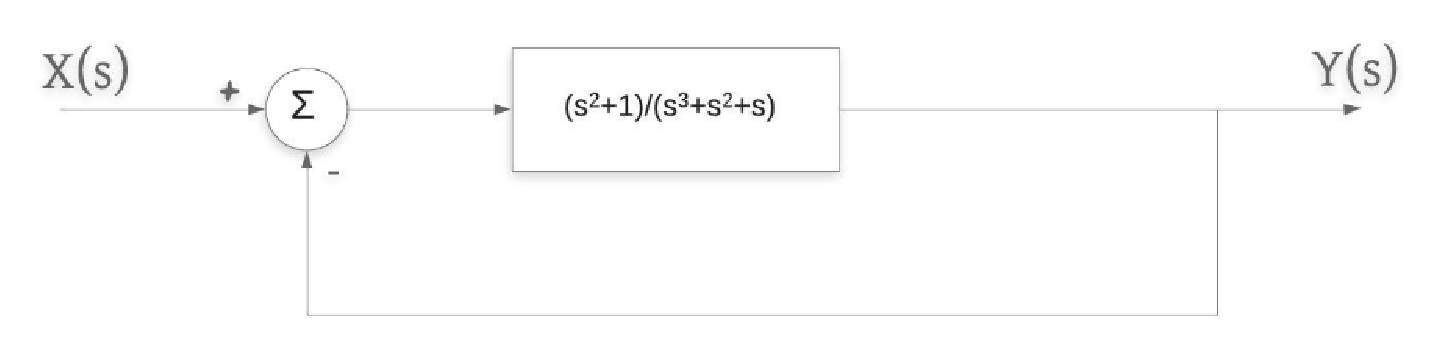
\includegraphics[width=0.5\textwidth]{./figs/pic6.eps}
\end{figure}
\\\\\\\\\\\\\\\\
Again we will solve this then we will get
\begin{figure}[h]
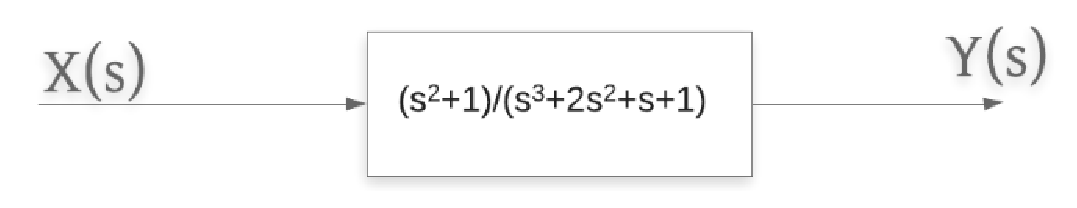
\includegraphics[width=0.5\textwidth]{./figs/pic8.eps}
\end{figure}

Now\\

X(s)($\frac{s^2+1}{s^3+2s^2+s+1}$)=Y(s)\\

$\frac{Y(s)}{X(s)}$=$\frac{s^2+1}{s^3+2s^2+s+1}$\\
\\
 The correct option is (B)
 \\\\
\begin{frame}{Question-4 }
Let the state-space representation of an LTI system be.
\\
\\ $\dot{x(t)}=Ax(t)+Bu(t)$
\\y(t)=Cx(t)+Du(t)
\\A,B,C are matrices, D is scalar, u(t) is input to the system and y(t) is output to the system. let 
$$b1 =\begin{vmatrix}
 0&0&1\\
\end{vmatrix}
$$ 
\\$b1^T=B$
\\and D=0. Find A and C.
\\
\\$H(s)=\dfrac{1}{s^3+3s^2+2s+1}$}
\\
\end{frame}
\\
\\\begin{frame}{Solution:- }
STATE MODEL
\\Let U1(t) and U2(t) are the inputs of the MIMO system and y1(t),y2(t) are the output of the system and x1(t) and x2(t) are the state variables. 
\\so output equation is,
\begin{equation}
    y1(t)=C_{11}\times x1(t)+C_{12}\times x2(t)+d_{11}\times U1(t)+d_{12}\times U2(t)
\end{equation}
\\
\begin{equation}
    y2(t)=C_{21}\times x1(t)+C_{22}\times x2(t)+d_{21}\times U1(t)+d_{22}\times U2(t)
\end{equation}
\\
\[
\begin{bmatrix}
y1(t)\\
y2(t)
\end{bmatrix}
=
\begin{bmatrix}
C_{11}&C_{12}\\
C_{11}&C_{12}\\
\end{bmatrix}\times \begin{bmatrix}
x1(t)\\
x2(t)\\
\end{bmatrix}
+
\begin{bmatrix}
d_{11}&d_{12}\\
d_{11}&d_{12}\\
\end{bmatrix} \times\begin{bmatrix}
U1(t)\\
U2(t)\\
\end{bmatrix}
\]
\\therefore Y(t)=C.X(t)+D.U(t)
\begin{equation}
    \dot{x1(t)}=a_{11}\times x1(t)+a_{12}\times x2(t)+b_{11}\times U1(t)+b_{12}\times U2(tx
\end{equation}
\begin{equation}
    \dot{x2(t)}=a_{21}\times x1(t)+a_{22}\times x2(t)+b_{21}\times U1(t)+b_{22}\times U2(t)
\end{equation}

\[
\begin{bmatrix}
\dot{x1(t)}\\
\dot{x2(t)}
\end{bmatrix}
=
\begin{bmatrix}
a_{11}&a_{12}\\
a_{11}&a_{12}\\
\end{bmatrix}\times \begin{bmatrix}
x1(t)\\
x2(t)\\
\end{bmatrix}
+
\begin{bmatrix}
b_{11}&b_{12}\\
b_{11}&b_{12}\\
\end{bmatrix} \times\begin{bmatrix}
U1(t)\\
U2(t)\\
\end{bmatrix}
\]
\\$therefore$  $\dot{X(t)}$=A.X(t)+B.U(t)
\\
\\\item \textbf{FINDING TRANSFER FUNCTION}
\\
\\ $So$, $\dot{X(t)}$=A.X(t)+B.U(t) $~be~$ $~equation~$ $~1~$
\\
\\ and  Y(t)=C.X(t)+D.U(t)        $~be~$ $~equation~$ $~2~$
\\
\\
\\ by applying laplace transforms on both sides of equation 1
\\
\\ we get
\\
\\S.X(S)-X(0)=A.X(S)+B.U(S)
\\
\\S.X(S)-A.X(S)=B.U(S)+X(0)
\\
\\(SI-A)X(S)=X(0)+B.U(S)
\\
\\X(S)=X(0)([SI-A])^-1 + B.([SI-A])^-1.U(S)
\\
\\ $~Laplace~$ $~transform~$ $~of~$ $~equation~$ $~2~$ $~and~$ $~sub~$ $X(s)$ 
\\
\\Y(S)=C.X(S)+D.U(S)
\\
\\Y(S)=C.[X(0)([SI-A])^-1 + B.([SI-A])^-1.U(S)]+D.U(S)
\\
\\If X(0)=0
\\
\\ then Y(S)=C.[B.([SI-A])^-1.U(S)]+D.U(S)
\\
\\ \dfrac{Y(S)}{U(S)}=C.[B.([SI-A])^-1]+D=H(S)
\bigskip
\\ As$~$ we$~$ know$~$ that
\bigskip
\\ $$Y(s)=H(s) \times U(s)= (\dfrac{1}{s^3+3s^2+2s+1}) \times U(s)$
\\
\\let X(S)=\dfrac{U(S)}{denominator}
\bigskip
\\ Y(S)=X(S)\times numerotor
\bigskip
\\s^3X(s)+3s^2X(s)+2sX(s)+X(s)=U(S)
\\
\[
\begin{bmatrix}
sx(s)\\
s^2x(s)\\
s^3x(s)
\end{bmatrix}
=
\begin{bmatrix}
0&1&0\\
0&0&1\\
-1&-2&-3
\end{bmatrix}\times \begin{bmatrix}
x(s)\\
sx(s)\\
s^2x(s)
\end{bmatrix}
+
\begin{bmatrix}
0\\
0\\
1
\end{bmatrix} \times U
\]
\\
\\ therfore$~~~~$ A=\begin{bmatrix}
0&1&0\\
0&0&1\\
-1&-2&-3
\end{bmatrix}
\bigskip
\\ Since Y(S)=X(S)\times numerator
\\ therefore Y(S)=X(S);
\\
\\Y=
\begin{bmatrix}
1&0&0
\end{bmatrix}\times \begin{bmatrix}
x(s)\\
sx(s)\\
s^2x(s)
\end{bmatrix} 
\\C=\begin{bmatrix}
1&0&0
\end{bmatrix}
\end{frame}
\\\\\\
\begin{frame}{Question-5 }
     {Consider a unity feedback system as shown in the figure,shown with an integral compensator k/s and open-loop transfer function} \\
G(s) = $\frac{1}{s^2+3s+2}$
\\
    where k$>$0. The positive value of k for which there are two poles of unity feedback system on j${\omega}$ {axis is equal to-----(rounded off to two decimal places)}
 
\begin{figure}[h]
     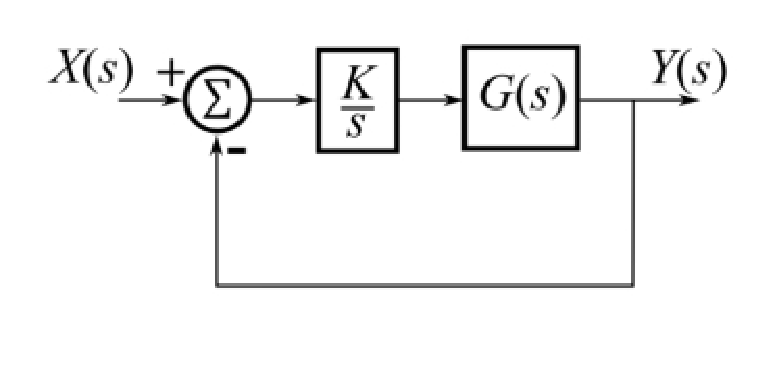
\includegraphics[width=\linewidth]{./figs/gate.eps}
    \end{figure}
\end{frame}
\\\\\\\\\\\\\\\\
\begin{frame}{Solution:- }
A transfer function is the relative function between input and output.
\newline In a negative feedback system an intermediate signal is defined as Z.
\begin{figure}
    \centering
    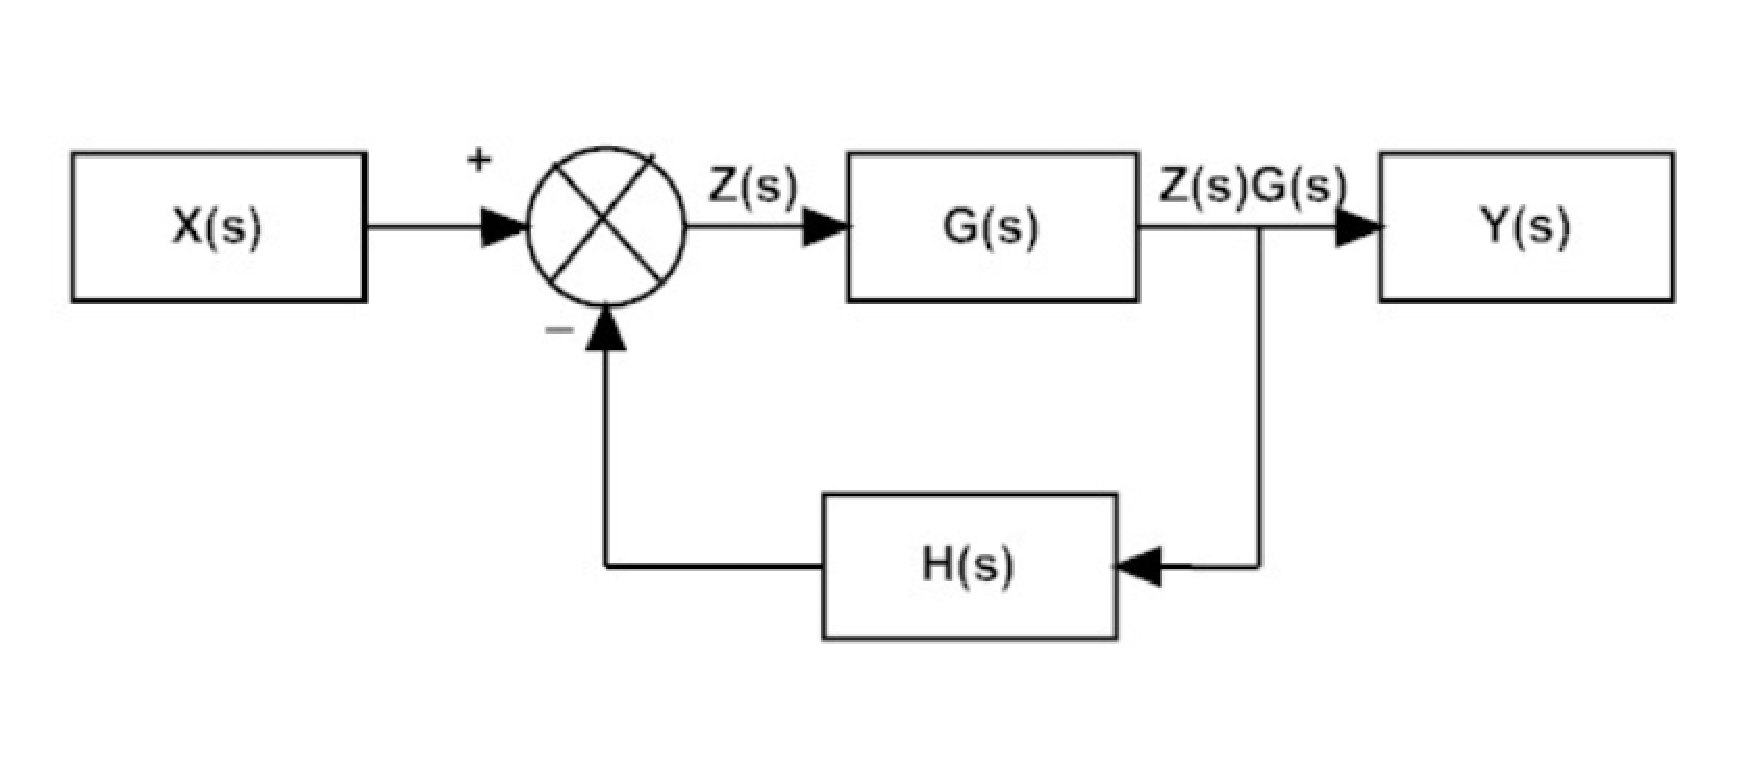
\includegraphics[width =\linewidth]{./figs/feedback.eps}
\end{figure}
\end{frame}
\begin{frame}
\\\\\\\\\\
Y(s) = Z(s).G(s)
\newline 
Z(s) = X(s) - Y(s).H(s) $\Rightarrow$ X(s) = Z(s)+Y(s).H(s)
\newline \\
X(s) = Z(s)+Z(s).G(s).H(s)
\newline \\
$\frac{Y(s)}{X(s)}$ = $\frac{Z(s).G(s)}{Z(s)+Z(s).G(s).H(s)}$

So,the transfer function of negative feedback is $\frac{G(s)}{1+G(s).H(s)}$
\newline Since unit feedback H(s) = 1
\newline Now the transfer function of unity negative feedback is $\frac{G(s)}{1+G(s)}$
\\
  The net transfer function in the given question is.....
  \newline
  
  $\frac{Y(s)}{X(s)}$ = $\frac{G(s)*k/s}{1+G(s)*k/s}$
  \newline
  
  The characteristic equation is 1 + (G(s)x$\frac{k}{s}$) = 0
 \newline that is..,
 \newline 
 
 C.E = 1 + $\frac{k}{s(s^2+3s+2)}$ = 0
 $\Rightarrow$ s(s^2+3s+2) + k = 0
 \newline 
 
$\Rightarrow$ s^3+3s^2+2s+k=0
\\Routh-Hurwitz  Criterion:-\\
\end{frame}
\begin{frame}{}
 This criterion is based on arranging the coefficients of characteristic equation intoan array called Routh array.
\\ 
 q(s) = $a_0$s^n+$a_1$s^{n-1}+$a_2$s^{n-2}+.....+$a_{n-1}$s+$a_n$ = 0
\newline 

\begin{vmatrix}s^n\\s^{n-1}\\s^{n-2} \\ \vdots \end{vmatrix} \begin{vmatrix}
a_0 & a_2 & a_4 & \cdots \\
a_1 & a_3 & a_5 & \cdots  \\
b_1 & b_2 & b_3 & \cdots \\
\vdots & \vdots & \vdots & \ddots &\vdots 
 \cdots \\ \end{vmatrix} 
 \\\\ where b_1 =\frac{ a_1a_2-a_0a_3}{a_1}  \hspace{5pt} b_2 =\frac{ a_1a_4-a_0a_5}{a_1} \\\\ c_1=\frac{ b_1a_3-a_1b_2}{b_1}  \hspace{5pt}     c_2=\frac{ b_1a_5-a_1b_3}{b_1}  
\\
\end{frame}
\begin{frame}{}
 For poles to lie on imaginary axis any one entire row of hurwitz matrix should be zero.
 \newline 
 
 For the given characteristic equation =  s^3+3s^2+2s+k = 0
 \newline \begin{vmatrix}s^3\\s^2\\s^1 \\ s^0 \end{vmatrix} \begin{vmatrix}
1 & 2 \\ 3 & k \\  \frac{6-k}{3} & 0\\ k & 0
\end{vmatrix}
\newline $For poles on $j$\omega$ axis any one of the row should be zero
\newline  $\Rightarrow$ $\frac{6-k}{3}$ = 0 or k = 0
\newline But given k$>$0 ...
\newline therefore, 6-k=0  $\Rightarrow$ k = 6
\\
To find the location of poles on j$\omega$ axis 
\newline 

Auxillary equation of the given CE is 3s^2 + k = 0
\newline
 $\Rightarrow$ 3s^2 + 6 = 0
\newline
 $\Rightarrow$ s = \pm j2
\\\\\ 
\end{frame}

\begin{frame} {Question-6 } 
 The output response of a system is denoted as y(t), and its Laplace transform is given by 
Y(s) = \dfrac{10}{s(s^2+ s + 100{(2)^{0.5})}}
\\
\end{frame}
\begin{frame}{}
The steady state value of y(t) is 
\\
a) 100(2)^{0.5}\hspace{4cm}
b) \dfrac{1}{10(2)^{0.5}} \\\\
c)  10(2)^{0.5} \hspace{4cm}
d) \dfrac{1}{100(2)^{0.5}}
\\
\end{frame}

\begin{frame}{Solution:- }


\begin{figure}[htp]
    
    The final value theorem states that  \[ \lim_{t \to \infty} y(t) = \lim_{s \to 0} sY(s)\]
\newline This is valid only when sY(s) has poles that lie in the negative half of the real side.
\end{figure}
 
  If the quadratic equation $ax^2 + bx + c$ has complex roots then the real part of those roots will be -b/2a
\\  
  Hence, verified that the roots of $s^2+ s + 100{(2)^{0.5}}$ have a negative real part which is -0.5. So, Final value theorem is applicable.
\\
 Steady state value of y(t) = \[ \lim_{t \to \infty} y(t) = \lim_{s \to 0} sY(s) = \lim_{s \to 0} \dfrac{10s}{s(s^2+ s + 100{(2)^{0.5})}} \]   
 \centering
 = \dfrac{10}{100(2)^{0.5}} =  \dfrac{1}{10(2)^{0.5}}
\end{frame}
\begin{frame}{}
\begin{figure}
    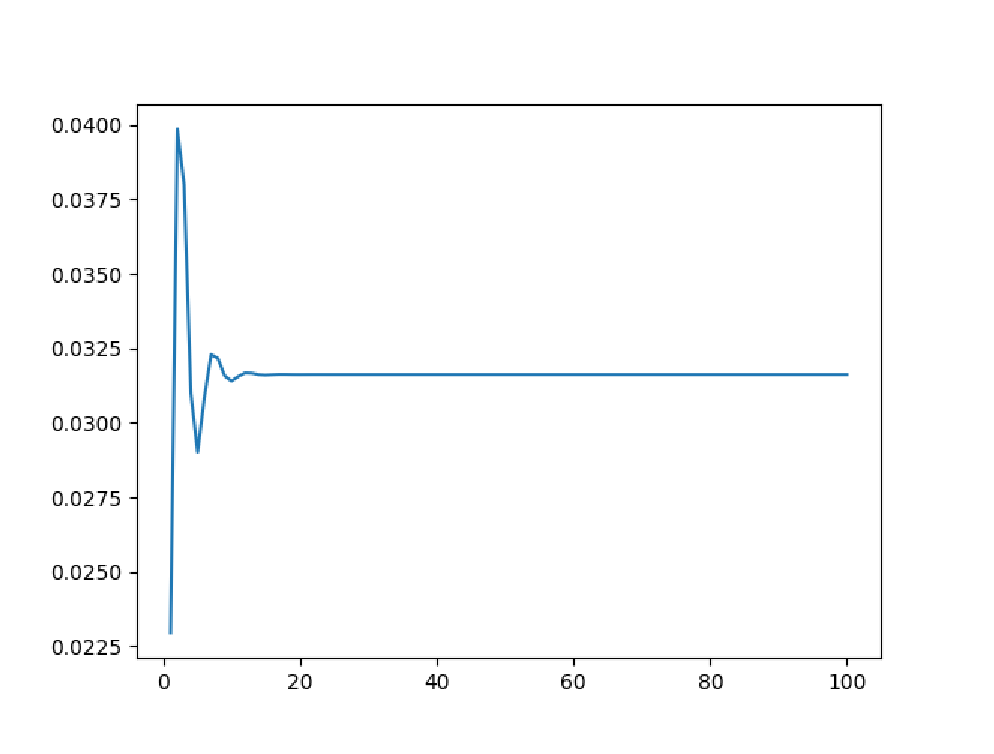
\includegraphics[width=8cm]{./figs/shru1.eps}
\end{figure}
\\\\\\\\\\\\
We can see that y(t) is approaching a constant value 0.031 which is verifies our answer!    
\end{frame} 

\begin{frame}{Question-7 }
\begin{itemize}
\item The open loop transfer function of a unity feedback system is given by
\begin{align*}
 G(s)=\frac{\pi e^{-0.25s}}{s}
\end{align*}
in G(s) plane,the Nyquist plot of G(s) passes through the negative real axis at the point
\\*(A)(-0.5,j0)  (B)(-0.75,j0)  (C)(-1.25,j0) \\ (D)(-1.5,j0)
\end{itemize}
\end{frame}
\begin{frame}{Solution:- }
\begin{itemize}


\begin{equation*}

G(s)=\frac{\pi e^{-0.25s}}{s}

\end{equation*}
 Nyquist plot cuts the negative real
Axis at $\omega$ = phase cross over frequency
\newline \(G(j\omega)=\frac{\pi}{\omega}(-\sin{0.25$\omega$}-j\cos{0.25$\omega$})\)
\newline \angle G(j$\omega$)=-90\degree-0.25$\omega$\times180\degree/$\pi$
\newline\angle G(j$\omega$)|$_{\omega=\omega_{pc}}$=-180\degree
\newline by solving for $\omega$ we get $\omega_{pc}=2\pi$
\newline magnitude at any point is X=$|G(j\omega)|$=$\frac{\pi}{\omega}$
\newline substituting $\omega=2\pi$ in magnitude we get X=0.5
\newline hence it intersects at (-0.5,0j) so answer is A

\end{itemize}
\end{frame}

\begin{frame}{}

\begin{figure}
  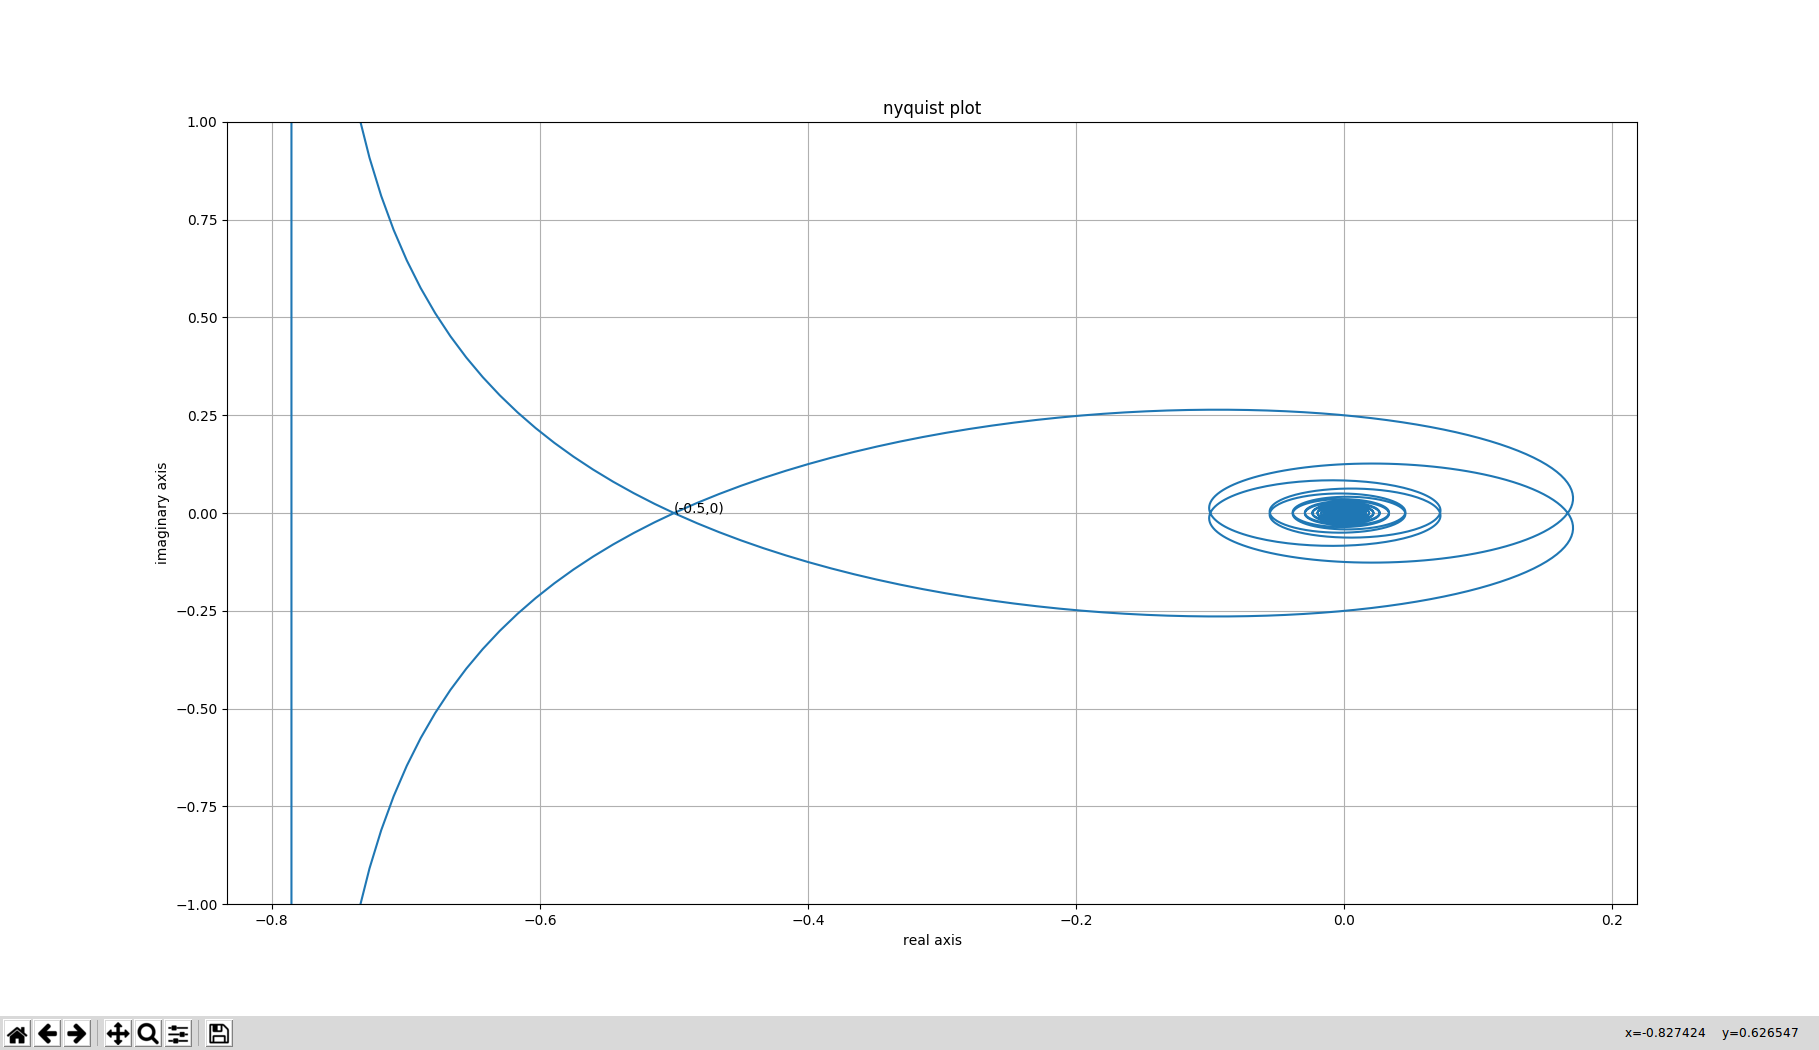
\includegraphics[width=\linewidth]{./figs/nyquist.eps}
\end{figure}

\newline we can verify with the following plot that it intersects at (-0.5,0j)


\\\\\\\\\\\\\\\\\\\\\\\\\\\
\\\\\\\\\\
\end{frame}


\begin{frame}{Question-8 }
The characteristic equation of linear time invariant system is given by 
$$\nabla(s)=s^4+3s^3+3s^2+s+k=0$$
\\The system is BIBO stable if}
\\A.0$<$k$<$\dfrac{12}{9}
\\
\\B.k>3
\\
\\C.0<k<\dfrac{8}{9}
\\
\\D.k>6
\end{frame}
\\\\
\begin{frame}{Solution:- }
\\
\\Given data: $$\nabla(s)=s^4+3s^3+3s^2+s+k=0$$
\\
\\
\\
\begin{tabular}{ |p{2cm}|p{2cm}|p{2cm}|p{1cm}|p{1cm}| }

 \hline
s^4 &1&3&K\\
 \hline
 s^3 & 3&1 & 0\\
 \hline
 s^2 & 8/3 & k & 0\\
 \hline 
 s & (8/3-3K)/(8/3) & 0 & 0\\
 \hline 
s^0 & k& 0& 0\\
\hline
\end{tabular}
\\
\\
\\ \Rightarrow \dfrac{\dfrac{8}{3}-3k}{\dfrac{8}{3}}>0
\\
\\
\\ \Rightarrow {\dfrac{8}{3}-3k} >0
\\
\\ \Rightarrow 3k<\dfrac{8}{9}
\\
\\ \Rightarrow (0<k<\dfrac{8}{9})
\\
\end{frame}
\begin{frame}{}
\\for example the zeros of polynomial s^4+3s^3+3s^2+s+0.5=0 are 
\\
\\  $$s1=−0.08373+0.45773i$$

\\ $$s2=−0.08373−0.45773i$$

\\$$s3=−1.41627+0.55075i$$

\\$$s4=−1.41627−0.55075i$$
\end{frame}

\begin{frame}{Question-9 }
The asymptotic Bode magnitude plot of  minimum phase transfer function
G(s) is show below.
\\\\
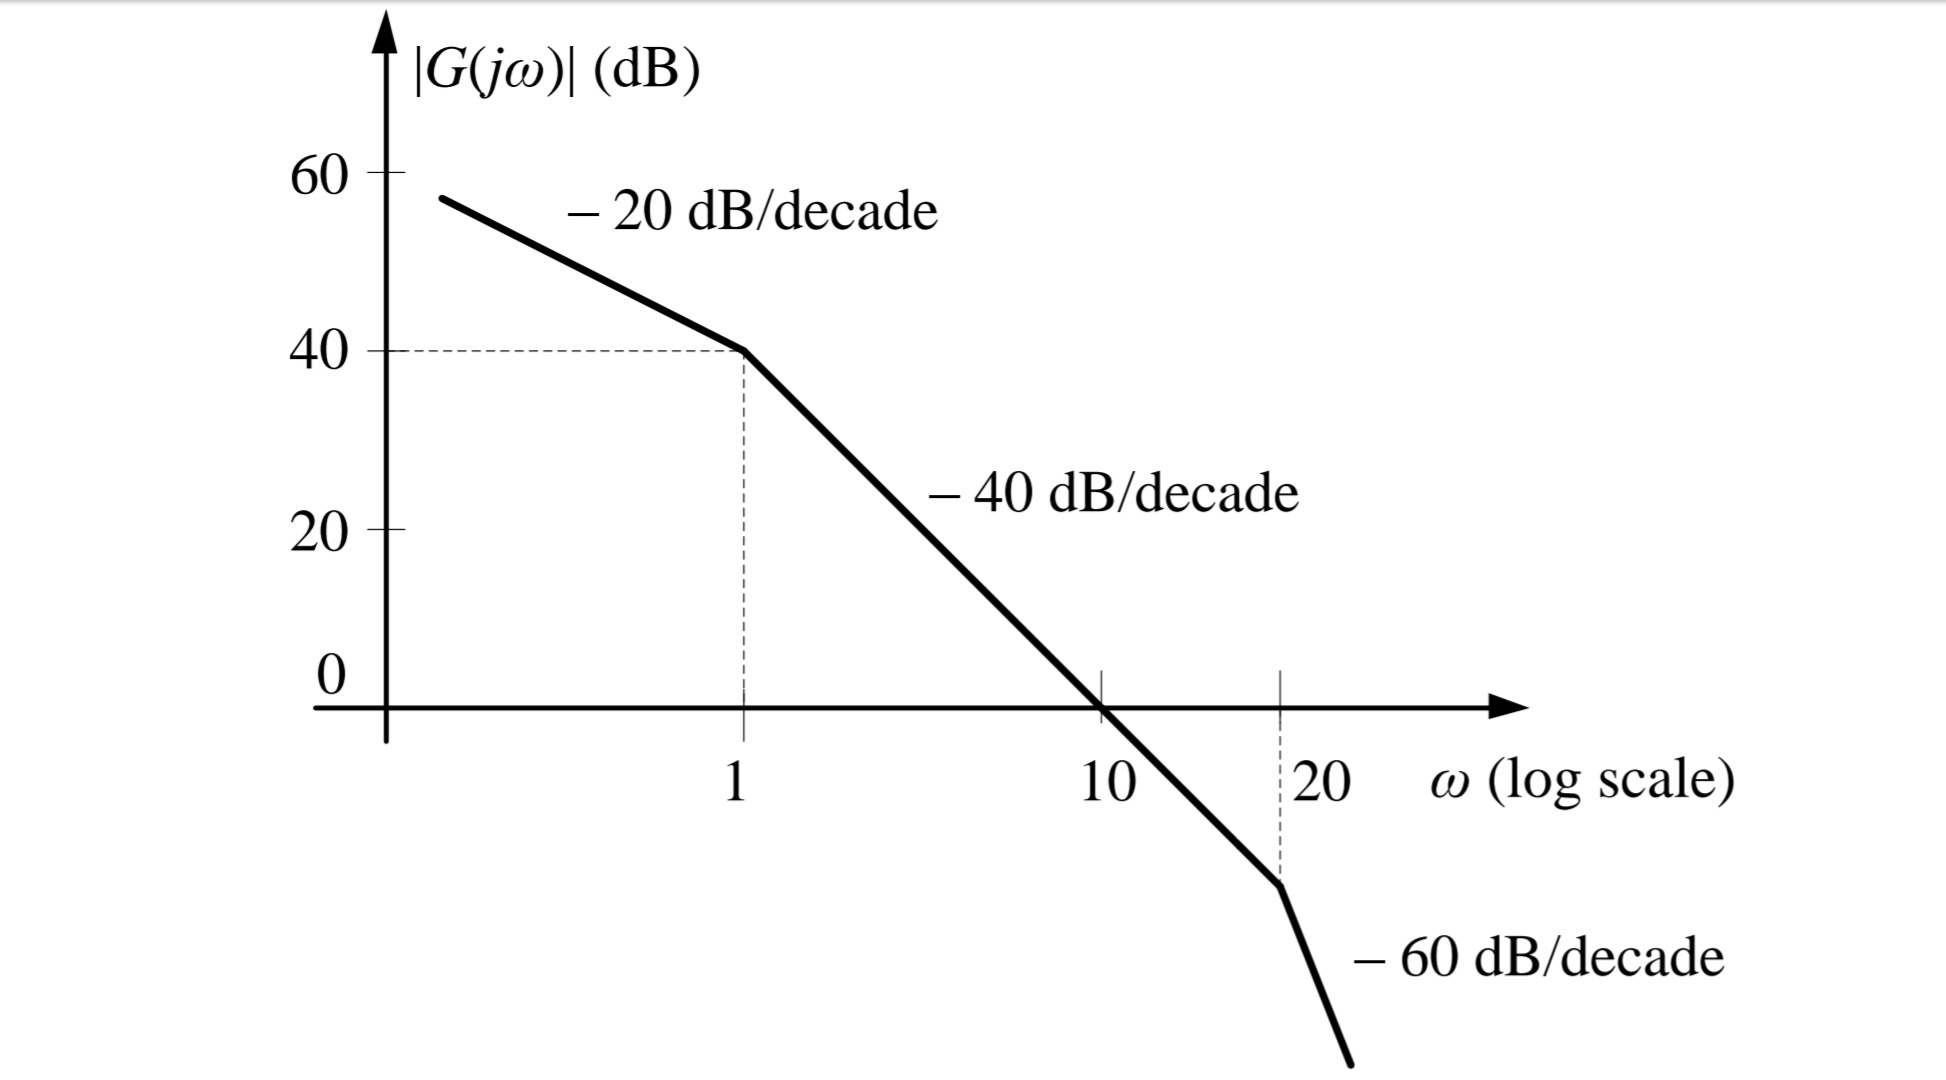
\includegraphics[scale = .12]{./figs/pppp.eps}
\end{frame}

\begin{frame}
\\\\  
Consider the following two statements.\\
\quad Statement 1: Transfer function G(s) has 3 poles and one zero \\
\quad Statement 2: At very high frequency $(\omega \to \infty)$, the phase \\  \quad \quad \quad \quad \quad \quad angle $ \angle G(j\omega)=-3\pi/2$ \\ 
Which of the following is correct ? \\
(A) Statement 1 is true and Statement 2 is false.\\
(B) Statement 1 is false and Statement 2 is true.\\
(C) Both the statements are true.\\
(D) Both the statements are false.
\\\\
\end{frame}


\begin{frame}{Solution:- }
Since, each pole corresponds to -20 dB/decade  
and each zero corresponds to +20 dB/decade.\\
Therefore, from the given Bode plot we can get the Transfer equation,\\
\[ G(s) = \frac{k}{s(1+s)(20+s)} \]
\\
Now, from the Transfer equation we can conclude that,
there are three poles (0, -1 and -20 ) and no zeros.\\
\quad \quad \quad $\therefore$ Statement 1 is false \quad \quad \quad ..........(1)




\end{frame}

%------------------------------------------------


\begin{frame}{}
Calculating phase\\
Since we know that,\\
phase $ \phi $ is the sum of all the phases corresponding to each pole and zero.\\
phase corresponding to pole is = \[ - tan^{-1}( \frac{imaginary}{real}) \]
phase corresponding to zero is = \[tan^{-1}( \frac{imaginary}{real})\]

\end{frame}
%------------------------------------------------



now take,\[  s = j\omega  \]\\

 \[ \Rightarrow  G(j\omega) =  \frac{k}{j\omega(1+j\omega)(20+j\omega)}\]
 \\
Therefore, \\
 \[  \phi =  -tan^{-1}( {\frac{\omega}{0}}) - tan^{-1}(\omega) - tan^{-1}( \frac{\omega}{20})\]

  \[ \phi =  - 90^\circ - tan^{-1}(\omega) - tan^{-1}( \frac{\omega}{20})\]
  \\
  \[\because \omega \to \infty\] 


 
 \begin{frame}{}
  \[ \phi =   - 90^\circ - 90^\circ - 90^\circ\]
 \[\phi = -270^\circ\ \]
 \[\phi = -3\pi/2 \] 
\quad \quad \quad $\therefore$ Statement 2 is true \quad \quad \quad \quad ........(2)\\
 thus, from (1) and (2) option (B) is correct.
\end{frame}
\\\\\\
\begin{frame}{Question-10 }
The transfer function of phase lead compensator is given by $$D(s) = \frac{3(s+\frac{1}{3T})}{(s+\frac{1}{T})}$$ 
The frequency (in rad/sec), at which $\angle D(j\omega)$ is maximum, is \\
\setlength{\lineskip}{1em}
\textbf{(a)} $\sqrt{\frac{1}{T^2}}$ \;\;\;\;\;\; \textbf{(b)} $\sqrt{\frac{1}{3T^2}}$ \;\;\;\;\;\; \textbf{(c)} $\sqrt{3T}$ \;\;\;\;\;\; \textbf{(d)}$\sqrt{3T^2}$
\end{frame}
\\\\
\begin{frame}{Solution:- }
 The basic requirement of the phase lead network is that all poles and zeros of the transfer function of the network must lie on (-)ve real axis interlacing each other with a zero located as the nearest point to origin.
   \newline
   \newline
 The given transfer fuction is $$D(s) = \frac{3(s+\frac{1}{3T})}{(s+\frac{1}{T})}$$
\end{frame}

\begin{frame}{}
  Now substituting $s = j\omega$ in D(s), we get\newline
   $$D(j\omega) = \frac{3(j\omega+\frac{1}{3T})}{(j\omega+\frac{1}{T})}$$ 
   The phase of this transfer function $\phi(\omega)$ is given by
   $$\phi(\omega) = \tan^{-1}(3\omega T)-\tan^{-1}(\omega T)$$
   $\phi(\omega)$ has its maximum at $\omega_c$ such that $\phi '(\omega_c)=0$, 
   $$\phi '(\omega_c) = \frac{3T}{1+(3\omega _c T)^2}-\frac{T}{1+(\omega _c T)^2}$$
   \end{frame}

%------------------------------------------------

\begin{frame}{}
  After simplification,
  $$\omega _c ^2T^2 = \frac{1}{3}$$
  $$\omega _c = \sqrt{\frac{1}{3T^2}}$$
  Hence \textbf{(b)} is the correct option.
\end{frame}
\\\\\\\
\begin{frame}{Question-11 }
\begin{description}[font=$\bullet$~\normalfont\scshape\color{blue!50!black}]
Consider a state-variable model of a system
$$\left[ \begin{array}{c} \dot{x}_1 \\ \dot{x}_2 
\end{array} 
\right] = 
\begin{bmatrix} 0 & 1 \\ -$\alpha$ & -2$\beta$ 
\end{bmatrix} 
\left[ 
\begin{array}{c} x_1 \\ x_2 
\end{array}
\right]
+
\left[
\begin{array}{c} b_1 \\ b_2 
\end{array}
\right]
r$$
$$y =  \begin{bmatrix} 1 & 0 \end{bmatrix}\left[ 
\begin{array}{c} x_1 \\ x_2 
\end{array}
\right]$$
where y is the output, and r is the input. The damping ratio $\zeta$ and the undamped natural
frequency $\omega_n$ (rad/sec) of the system are given by:
\begin{tabular}{cc}
    (A) \zeta = \dfrac{\beta}{\sqrt{\alpha}} , \omega_n = \sqrt{\alpha} &  \\
    (B) \zeta = \sqrt{\alpha} , \omega_n = \dfrac{\beta}{\sqrt{\alpha}} &  \\
    (C) \zeta = \dfrac{\alpha}{\sqrt{\beta}} , \omega_n = \sqrt{\beta}  &  \\
    (D) \zeta = \sqrt{\beta} , \omega_n = \sqrt{\alpha}  &  \\
    
    \end{tabular}

\end{description}
\end{frame}
\\\\\\\
\begin{frame}{Solution:- }
 Transformation of State Equations to a Single Differential Equation
\begin{description}[font=$\bullet$~\normalfont\scshape\color{red!50!black}]
The state equations $\dot{x}$ =Ax+Br for a linear second-order system with a single input are a pair of coupled first-order differential equations in the two state variables:
\left[ \begin{array}{c} \dot{x}_1 \\ \dot{x}_2 
\end{array} 
\right] = 
\begin{bmatrix} a_1_1 & a_1_2 \\ a_2_1 & a_2_2 
\end{bmatrix} 
\left[ 
\begin{array}{c} x_1 \\ x_2 
\end{array}
\right]
+
\left[
\begin{array}{c} b_1 \\ b_2 
\end{array}
\right]
r.
\end{description}
\begin{description}
Or
\end{description}
\begin{description}
$$\dfrac{dx_1}{dt}= a_1_1x_1 + a_1_2x_2 + b_1r.$$
\end{description}
\begin{description}
$$\dfrac{dx_2}{dt}= a_2_1x_1 + a_2_2x_2 + b_2r.$$
\end{description}
\begin{description}
The state-space system representation may be transformed into a single differential equation ineither of the two state-variables.
\end{description}

\end{frame}

\begin{frame}
\frametitle{Transformation of State Equations to a Single Differential Equation}
\begin{description}[font=$\bullet$~\normalfont\scshape\color{red!50!black}]
 Taking the Laplace transform of the state equations
$$(sI - A)X(s)  =  BR(s)$$
\end{description}
\begin{description}
$$X(s)  =  (sI - A)^-^1BR(s)$$
\end{description}
\begin{description}
$$X(s)  = \frac{1}{det[sI - A]}\begin{bmatrix} s - a_2_2 & a_1_2 \\ a_2_1 & s - a_1_1 
\end{bmatrix}\left[\begin{array}{c} b_1 \\ b_2\end{array}\right]R(s) $$
\end{description}
\begin{description}
$$det [sI - A]X(s) = \begin{bmatrix} s - a_2_2 & a_1_2 \\ a_2_1 & s - a_1_1 
\end{bmatrix}\left[\begin{array}{c} b_1 \\ b_2\end{array}\right]R(s)$$
\end{description}
\end{frame}

\begin{frame}
\frametitle{Transformation of State Equations to a Single Differential Equation}
\begin{description}[font=$\bullet$~\normalfont\scshape\color{red!50!black}]
from this we can write
\end{description}
\begin{description}
\Rightarrow $$\dfrac{d^2x_1}{dt^2} - (a_1_1 + a_2_2)\dfrac{dx_1}{dt} + (a_1_1a_2_2 - a_1_2a_2_1)x_1  \\ = b_1\dfrac{du}{dt} + (a_1_2b_2 - a_2_2b_1)r.$$
\\
and
\\
\Rightarrow 
$$\dfrac{d^2x_2}{dt^2} - (a_1_1 + a_2_2)\dfrac{dx_2}{dt} + (a_1_1a_2_2 - a_1_2a_2_1)x_2 \\ = b_2\dfrac{du}{dt} + (a_2_1b_1 - a_1_1b_2)r.$$
\end{description}

\begin{description}
which can be written in terms of the two parameters $\omega_n$ and $\zeta$ as follows: 
\end{description}
\end{frame}

\begin{frame}
\frametitle{Transformation of State Equations to a Single Differential Equation}
\begin{description}[font=$\bullet$~\normalfont\scshape\color{red!50!black}]
$$\dfrac{d^2x_1}{dt^2} + 2\zeta\omega_n\dfrac{dx_1}{dt} + \omega_n^2x_1 = b_1\dfrac{du}{dt} + (a_1_2b_2 - a_2_2b_1)r.$$
and
$$\dfrac{d^2x_2}{dt^2} + 2\zeta\omega_n\dfrac{dx_2}{dt} + \omega_n^2x_1 = b_2\dfrac{du}{dt} + (a_2_1b_1 - a_1_1b_2)r.$$
\end{description}

\begin{description}
where $\zeta$ is the system(dimensionless) damping ratio and the undamped natural frequency with units of radian/second is \omega_n.
\end{description}
\begin{description}
By comparing above equations we get that:
$$\omega_n = \sqrt{a_1_1a_2_2 - a_1_2a_2_1}$$
and
$$\zeta = -\dfrac{(a_1_1+a_2_2)}{\omega_n} = \dfrac{-(a_1_1 + a_2_2)}{2\sqrt{a_1_1a_2_2 - a_1_2a_2_1}}$$
\end{description}
\end{frame}
\begin{frame}
\frametitle{Transformation of State Equations to a Single Differential Equation}
\begin{description}[font=$\bullet$~\normalfont\scshape\color{red!50!black}]
Now putting the give values in the variables we get,
\begin{tabular}{cc}
     & \\
    \zeta = \dfrac{-(0 - 2\beta)}{2\sqrt{0(-2\beta) - 1(-\alpha)}} = \dfrac{\beta}{\sqrt{\alpha}} &  \\
     & \\
    \omega_n = \sqrt{0(-2\beta) - 1(-\alpha)} = \sqrt{\alpha} & \\
     & \\
    So the answer is Option(A).
    \\\\\
\end{tabular}
\end{description}
\end{frame}

\begin{frame}{Question-12 }
Match the transfer functions of the second-order systems with the nature of the systems given below
\newline \underline{Transfer functions}
\hspace{5mm}
\underline{Systems}
\vspace{5mm}
\newline P &:$\frac{15}{{s^2+5s+15}}$
\hspace{5mm}
1:Overdamped
\vspace{2mm}
\newline Q &:$\frac{25}{{s^2+10s+25}}$
\hspace{5mm}
2:critically damped
\vspace{2mm}
\newline R &:$\frac{35}{{s^2+18s+35}}$
\hspace{5mm}
3:Underdamped
\\
\begin{itemsize}
\item (A)P-1,Q-2,R-3
\item (B)P-2,Q-1,R-3
\item (C)P-3,Q-2,R-1
\item (D)P-3,Q-1,R-2


\end{itemsize}
\end{frame}
\\
\begin{frame}{Solution:- }

The standard transfer function H(s)=$\frac{\omega^2}{s^2+2\zeta\omega+\omega^2}\\
where \\"\omega"\hspace{2mm} is \hspace{2mm} natural \hspace{2mm} frequency \\ and "\zeta" \hspace{2mm}is\hspace{2mm} damping\hspace{2mm} factor\\
\vspace{2mm}

\newline then compare the given functions with this we get\\
\vspace{5mm}

  1. For Transfer function H(s)=$\frac{15}{s^2+5s+15}$, \\
\begin{align*}
     \omega^2 &= 15 \\ 2\zeta\omega &=5\\
    \text{then we get } \zeta &=$\sqrt{\frac{5}{12}} \textless 1
\end{align*}
\end{frame}
\begin{frame}{}
2. For Transfer function H(s)=$\frac{25}{s^2+10s+25}$,\\
\begin{align*}
     \omega^2 &= 25 \\ 2\zeta\omega &=10\\
    \text{then we get } {\zeta} &= $\sqrt{\frac{5}{5}} = 1
\end{align*}
3. For Transfer function H(s)=$\frac{35}{s^2+18s+35}$,\\
\begin{align*}
    \omega^2 &= 35 \\ 2\zeta\omega &=18\\
    \text{then we get } {\zeta} &= $\sqrt{\frac{81}{35}} \textgreater 1
\end{align*}
\end{frame}
\begin{frame}{}
The damping of a system can be described as being one of the following:
 
\begin{block}{Overdamped}
The system returns to equilibrium without oscillating.For this
\zeta \textgreater 1.

\end{block}
 
\begin{block}{Critically damped}
The system returns to equilibrium as quickly as possible without oscillating.For this \zeta = 1 \\\\
\end{block}
\end{frame}
\begin{frame}{}
\begin{block}{Underdamped}
The system oscillates(at reduced frequency compared to the undamped case) with the amplitude gradually decreasing to zero.For this 0 \textless\zeta\textless1
\\\\
\end{block}
\begin{block}{Undamped}
The system oscillates at its natural resonant frequency(\omega0). For this $\zeta=0$
\\\\
\end{block}    
\end{frame}
\begin{frame}{}
 As for P:$\zeta \textless 1$
It is Underdamped system\\
As for Q: $\zeta =1$
It is critically damped system.\\
 As for R: $\zeta \textgreater 1$
It is an overdamped system.\\
\vspace{10mm}
So,P-3,Q-2,R-1. Option (C) is correct.
\end{frame}
\begin{frame}{}
\begin{figure}
    \centering
    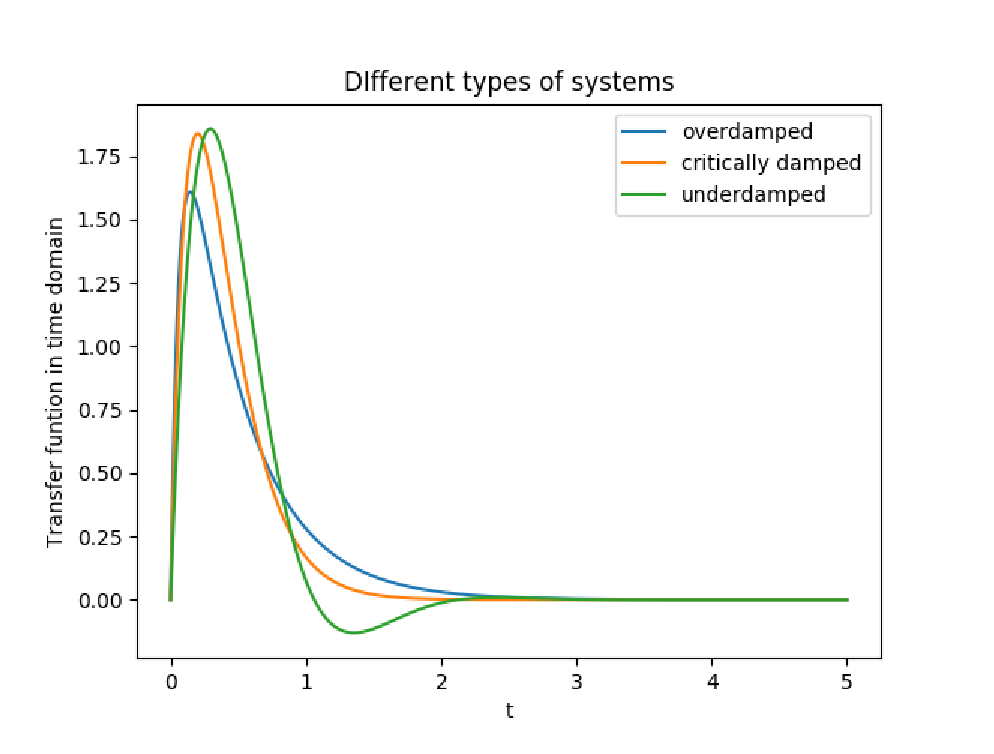
\includegraphics[width=1.1\linewidth]{./figs/Damping.eps}
\end{figure}
\end{frame}
\\\\\\
\begin{frame}{Question-13 }
The number of roots of the polynomial, $s^{7}+s^{6}+7 s^{5}+14 s^{4}+31s^{3}+73 s^{2}+25 s+$ $200,$ in the open left half of the complex plane is

(A) 3

(B) 4

(C) 5

(D) 6
\end{frame}
\\\\
\begin{frame}{Solution:- }

We will be using the concept of Routh-Hurwitz Criterion.

\textbf{Routh-Hurwitz Criterion:} The number of roots of the polynomial that are in the right half-plane is equal to
the number of sign changes in the first column.

\begin{itemize}
\item Routh–Hurwitz stability criterion is a mathematical test that is a necessary and sufficient condition for the stability of a linear time invariant control system.
\end{itemize}
\end{frame}


\begin{frame}{}

Rules for generating Routh-Hurwitz Table.

\begin{enumerate}
    \item Label the rows of Routh table from highest power to the lowest power.
    \item List alternative coefficients starting with the highest order coefficients in the first row.
    \item List alternative coefficients starting with the next highest order coefficients in the second row.
    \item Each entry is the negative of determinant of the previous two entries in the previous two rows divided by the entry in the first column directly above the row.
    \item The left hand column of the determinant is always the first column of the previous two rows.
    \item The right hand column is the elements of the column above and to the right.
    \item The table is complete when all of the rows are completed down to $s^0$.
\end{enumerate}
\end{frame}
\\
\begin{frame}{}
The Routh-Hurwitz Table for given equation $s^{7}+s^{6}+7 s^{5}+14 s^{4}+31s^{3}+73 s^{2}+25 s+$ $200,$ is calculated as follows

\begin{table}[h]
\begin{tabular}{|C{2cm}|a{2cm}|b{2cm}|c{2cm}|d{2cm}|}
\hline
$s^7$ & 1 & 7 & 31 & 25\\
\hline
$s^6$ & 1 & 14 & 73 & 200\\
\hline
\end{tabular}
\end{table}

\begin{table}[h]
\begin{tabular}{|C{2cm}|a{2cm}|b{2cm}|c{2cm}|d{2cm}|}
\hline
$s^7$ & 1 & 7 & 31 & 25\\
\hline
$s^6$ & 1 & 14 & 73 & 200\\
\hline
$s^5$ & -7 & -42 & -175 & 0\\
\hline
\end{tabular}
\end{table}
\end{frame}
\begin{frame}{}
\begin{table}[h!]
\begin{tabular}{|C{2cm}|a{2cm}|b{2cm}|c{2cm}|d{2cm}|}
\hline
$s^7$ & 1 & 7 & 31 & 25\\
\hline
$s^6$ & 1 & 14 & 73 & 200\\
\hline
$s^5$ & -7 & -42 & -175 & 0\\
\hline
$s^4$ & 8 & 48 & 200 & 0\\
\hline
\end{tabular}
\end{table}
\begin{table}[h!]
\begin{tabular}{|C{2cm}|a{2cm}|b{2cm}|c{2cm}|d{2cm}|}
\hline
$s^7$ & 1 & 7 & 31 & 25\\
\hline
$s^6$ & 1 & 14 & 73 & 200\\
\hline
$s^5$ & -7 & -42 & -175 & 0\\
\hline
$s^4$ & 8 & 48 & 200 & 0\\
\hline
$s^3$ & 0 & 0 & 0 &  \\
\hline
\end{tabular}
\end{table}
\end{frame}
\begin{frame}{}
\\\\\\
When such a case is encountered, we take the derivative of the expression formed the the coefficients above it i.e derivative of $8s^4 + 48s^2 +200$.\\
\begin{center}
$\frac{d}{dx}(8s^4 + 48s^2 +200) = 32s^3 + 96s$
\end{center}
The coefficients of obtained expression are placed in the table. 
\begin{frame}{}
\begin{table}
\begin{tabular}{|C{2cm}|a{2cm}|b{2cm}|c{2cm}|d{2cm}|}
\hline
$s^7$ & 1 & 7 & 31 & 25\\
\hline
$s^6$ & 1 & 14 & 73 & 200\\
\hline
$s^5$ & -7 & -42 & -175 & 0\\
\hline
$s^4$ & 8 & 48 & 200 & 0\\
\hline
$s^3$ & 32 & 96 & 0 &  \\
\hline
\end{tabular}
\end{table}
\begin{table}
\begin{tabular}{|C{2cm}|a{2cm}|b{2cm}|c{2cm}|d{2cm}|}
\hline
$s^7$ & 1 & 7 & 31 & 25\\
\hline
$s^6$ & 1 & 14 & 73 & 200\\
\hline
$s^5$ & -7 & -42 & -175 & 0\\
\hline
$s^4$ & 8 & 48 & 200 & 0\\
\hline
$s^3$ & 32 & 96 & 0 &  \\
\hline
$s^2$ & 24 & 200 & 0 &  \\
\hline
\end{tabular}
\end{table}
\begin{table}[h!]
\begin{tabular}{|C{2cm}|a{2cm}|b{2cm}|c{2cm}|d{2cm}|}
\hline
$s^7$ & 1 & 7 & 31 & 25\\
\hline
$s^6$ & 1 & 14 & 73 & 200\\
\hline
$s^5$ & -7 & -42 & -175 & 0\\
\hline
$s^4$ & 8 & 48 & 200 & 0\\
\hline
$s^3$ & 32 & 96 & 0 & \\
\hline
$s^2$ & 24 & 200 & 0 & \\
\hline
$s^1$ & -170.67 & 0 &  & \\
\hline
\end{tabular}
\end{table}
\end{frame}
\begin{frame}{}
\begin{table}[h!]
\begin{tabular}{|C{2cm}|a{2cm}|b{2cm}|c{2cm}|d{2cm}|}
\hline
$s^7$ & 1 & 7 & 31 & 25\\
\hline
$s^6$ & 1 & 14 & 73 & 200\\
\hline
$s^5$ & -7 & -42 & -175 & 0\\
\hline
$s^4$ & 8 & 48 & 200 & 0\\
\hline
$s^3$ & 32 & 96 & 0 & \\
\hline
$s^2$ & 24 & 200 & 0 & \\
\hline
$s^1$ & -170.67 & 0 &  & \\
\hline
$s^0$ & 200 &   &   & \\
\hline
\end{tabular}
\end{table}
\end{frame}

\begin{frame}
\\\\\\\\\\\\\\\\\\
So, the above one is the Routh-Hurwitz Table.
The no.of sign changes in first column of Routh–Hurwitz Table is the no.of roots on right side of imaginary axis.

So, for the given equation 4 roots lie on right-side of Imaginary Axis.

Given equation has a total of 7 roots in which 4 lie on right side of Imaginary Axis. \textbf{So there will be 3 roots on left of Imaginary Axis.}
    
\end{frame}

\begin{frame}{}
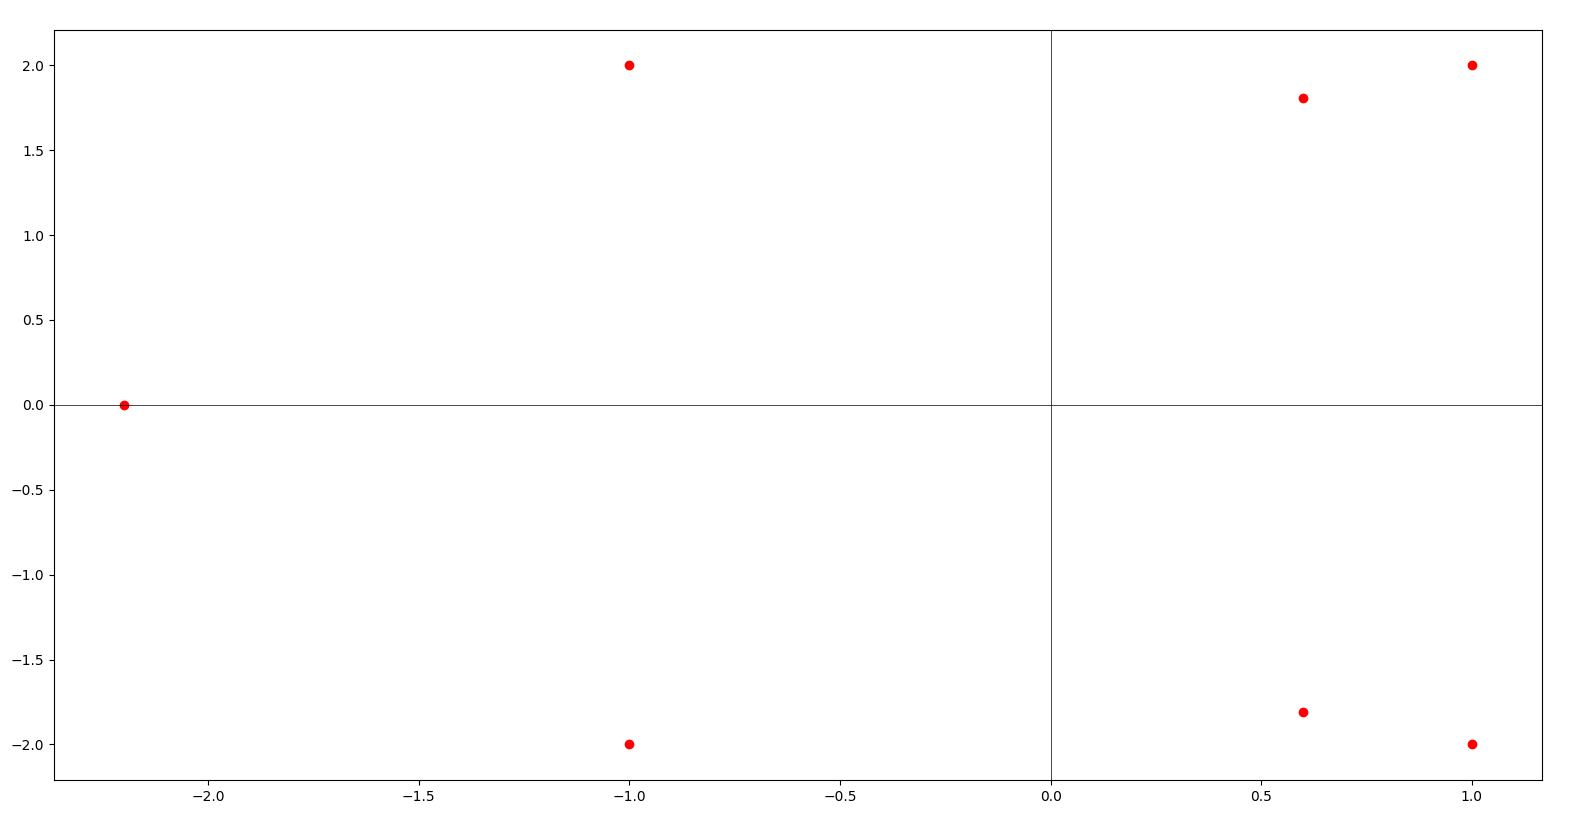
\includegraphics[scale=0.15]{./figs/Roots.eps}
\end{frame}
\\\\\\
\begin{frame}{Question-14 }
The unit step response of y(t) of a unity feedback system with an open loop transfer function  
\[ G(s)H(S)=\frac{K}{(s+1)^2(s+2)}  \]
is shown in figure. The value of K is(up to two decimal places).
\end{frame}
\begin{frame}{}
\begin{figure}[h]
    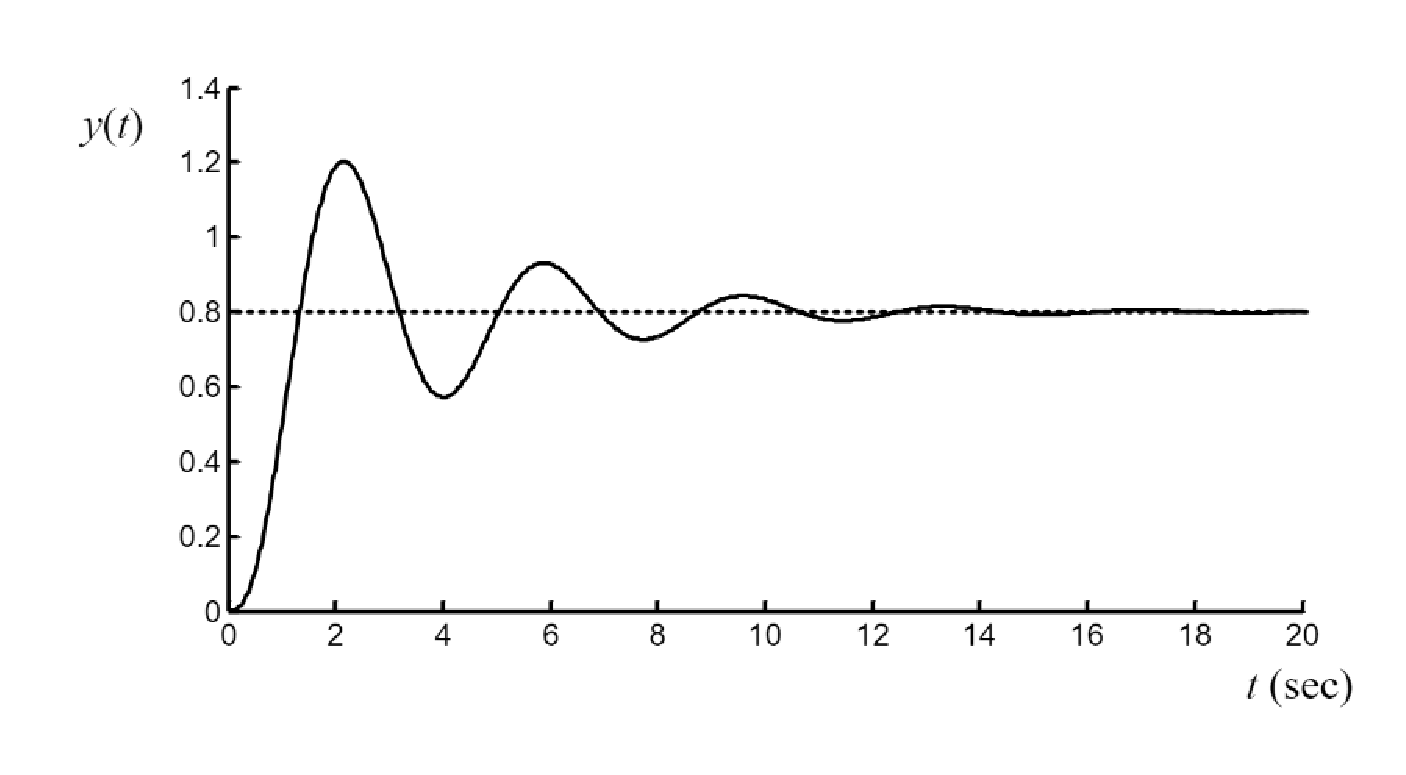
\includegraphics[width=10cm, height=8cm]{./figs/Screenshot(32).eps}    
\end{figure}
\end{frame}
\\\\\
\begin{frame}{Solution:- }
Given,
\[ G(s)H(s)=\frac{K}{(s+1)^2(s+2)}  \]
We know that the input and output relation for open loop transfer function for a unity feedback system is given by,
\[ \frac{Y(s)}{X(s)}=\frac{G(s)}{1+G(s)H(s)}=\frac{G(s)}{1+G(s)}\]
Now, substituting the G(s)H(s) in the above equation we will get the below,
\[ \frac{Y(s)}{X(s)}=\frac{\frac{K}{(s+1)^2(s+2)}}{1+\frac{K}{(s+1)^2(s+2)}}\]
\end{frame}
\begin{frame}{}
  \[ \frac{Y(s)}{X(s)}=\frac{K}{K+(s+1)^2(s+2)}  \]
According to the question, \[X(s)=\frac{1}{s}\]
So,\[Y(s)=\frac{1}{s} \  \frac{K}{K+(s+1)^2(s+2)}\]
From final value theorem,
\[y(\infty\;)=\lim_{s \rightarrow 0 }sY(s)=0.8\]
[From the response shown in the figure steady state value in the time domain is 0.8]
\end{frame}
\begin{frame}{}
\[\frac{K}{K+2}=0.8\]\\
\[K=1.6+0.8K\]\\
\[K=8\]\\
Hence,the value of K is 8
\end{frame}
\\\\\\
\begin{frame}{Question-15 }
An input p(t) = sin(t) is applied to the system $G(s) = \frac{s-1}{s+1} $. The corresponding steady state output is y(t) = sin(t + $\varphi$), where the phase $\varphi$ (in degrees), when restricted to 0$^{\circ}$ $\leq$ $\varphi$ $\leq$ 360$^{\circ}$, is ?
\end{frame}
\\\\
\begin{frame}{Solution:- }

\vspace{4 mm}
We have p(t) = sin(t)

\vspace{4 mm}
We know that Laplace Transform of p(t) = $\mathcal{L}$(p(t)) = P(s)

\vspace{2 mm}
So , P(s) = $\frac{1}{s^2 + 1}$

\vspace{4 mm}

And we are given the steady state output $y_s(t)$ = sin(t+$\varphi$) 

\vspace{4 mm}
So , y_s(t) = sin(t)cos($\varphi$) + cos(t)sin($\varphi$) , 

\vspace{4 mm}
 Hence Laplace transform of y(t) in steady state = $\mathcal{L}$(y_s(t)) = Y_s(s) = \mathcal{L}(sin(t))cos($\varphi$) + $\mathcal{L}$(cos(t))sin($\varphi$)
 
\end{frame}

\begin{frame}{}
\vspace{4 mm}
Since , $\mathcal{L}$(sin(t)) = $\frac{1}{s^2 + 1}$ And $\mathcal{L}$(cos(t)) = $\frac{s}{s^2 + 1}$

\vspace{4 mm}
So , Y_s(s) = \frac{cos\varphi + s(sin\varphi)}{s^2 + 1} 

\vspace{4 mm}
And G(s) = $\frac{s-1}{s+1}$

\vspace{4 mm}
Hence , the output of the system in s-domain is Y(s) = P(s)G(s) 

\vspace{4 mm}
So , Y(s) = $\frac{1}{s^2 + 1}$ . $\frac{s-1}{s+1}$ , For solving this we can use the partial fractions :

\end{frame}

\begin{frame}{}
\vspace{4 mm}

Y(s) = $\frac{As + B}{s^2 + 1}$ + $\frac{C}{s + 1}$ = $\frac{(A+C)s^2 + (A+B)s + (B+C)}{(s^2 + 1)(s + 1)}$  

\vspace{4 mm}
Hence , by comparing coefficients ,

\vspace{4 mm }
we get A+C = 0 , A+B = 1 , B+C = -1

\vspace{4 mm}
After solving these above equations , we get A = 1 , B = 0 , C = -1. 

\vspace{4 mm}
So , Y(s) =  $\frac{s}{s^2 + 1}$ - $\frac{1}{s + 1}$

\vspace{4 mm}
Now we know that Laplace transform of e^{-t}u(t) = \mathcal{L}(e^{-t}u(t)) = \frac{1}{s+1}
\end{frame}

\begin{frame}{}
\vspace{4 mm}
i.e $\mathcal{L}$^{-1}(\frac{1}{s+1}) = e^{-1}u(t)


\vspace{4 mm}
 As for steady state analysis , we put t $\rightarrow$ $\infty$ ,therefore $e^{-1}u(t)$ will disappear while taking inverse laplace transform . Hence in steady state , only $\frac{s}{s^2 + 1}$ term will appear in laplace transform of y(t) as t $\rightarrow$ $\infty$

\vspace{4 mm}
Hence , in steady state , Y(s) = $\frac{s}{s^2 + 1}$ = $Y_s(s)$ given previously.

\vspace{4 mm}
So , $\frac{s}{s^2 + 1}$ = $\frac{cos(\varphi) + s(cos(\varphi))}{s^2 + 1}$

\vspace{4 mm}
By comparing coefficients of s and constants , we get $cos(\varphi)$ = 0 and $sin(\varphi)$ = 1 

\vspace{4 mm}

 

 So, because 0$^{\circ}$ $\leq$ $\varphi$ $\leq$ 360$^{\circ}$ , therefore $\varphi$ = 90$^{\circ}$


\end{frame}

\begin{frame}{}

Plot obtained for verification in python :
\setlength{\parindent}{1cm}
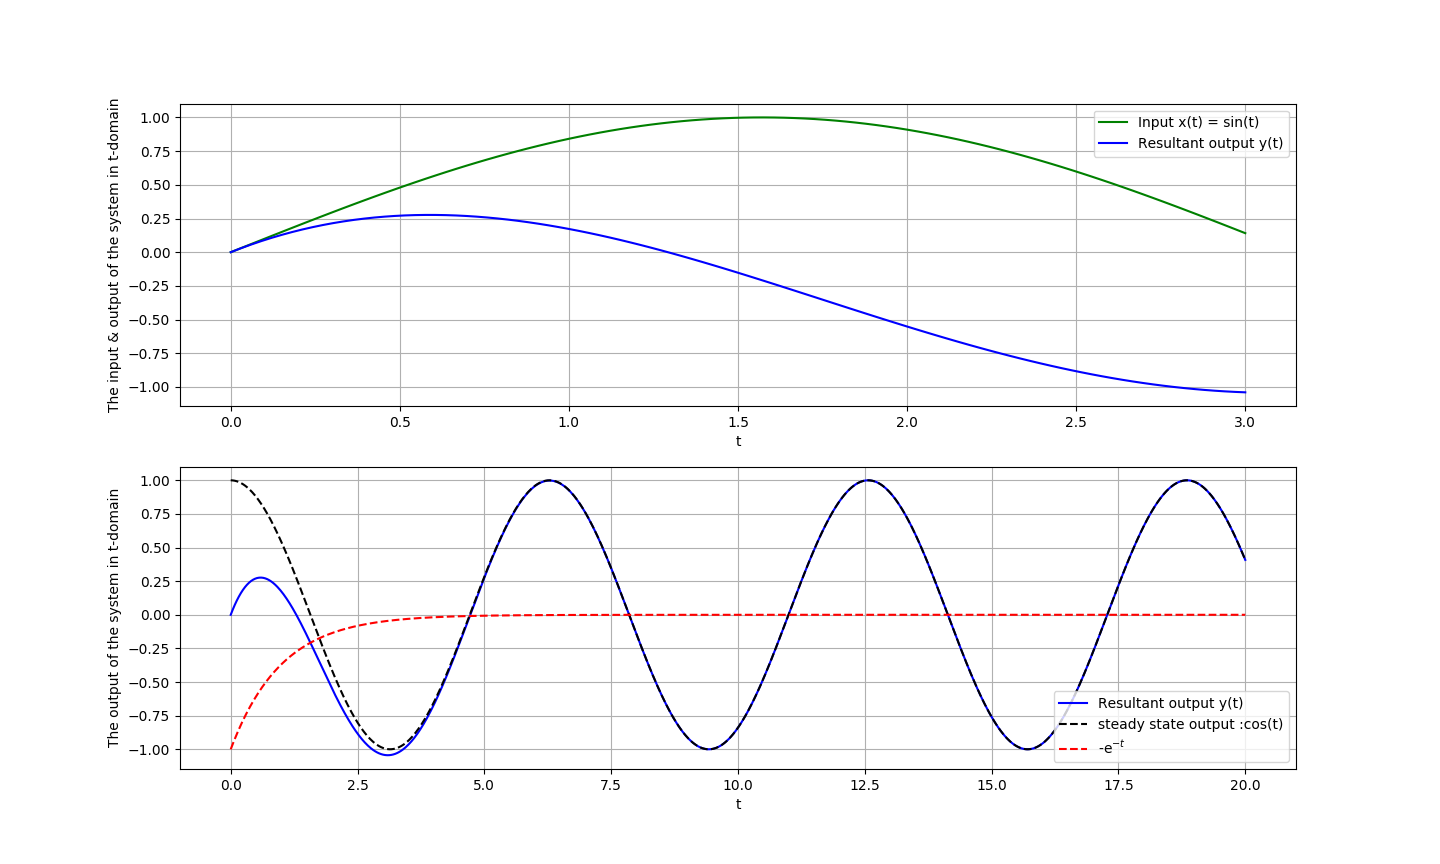
\includegraphics[scale=0.25]{./figs/Output_plot.eps}

\end{frame}
\begin{frame}{}
In above plot , black color plot is of cos(t).And blue color plot is the plot of resultant y(t) .So , we can see from above plots that black and blue color plots are coinciding after t = 3 . Hence y(t) = sin(t + 90$^{\circ}$) in steady state.
\end{frame}
\\\\\\\\
\begin{frame}{Question-16 }
Consider the transfer function $G(s)=\frac{2}{(s+1)(s+2)}$ . The Phase Margin of $G(s)$ in degrees is
\underline{\hspace{1.5cm}}}
\\\\\\
\end{frame}
%\frame{\titlepage} 
\begin{frame}{Solution:- }
\textbf{Gain Margin:}The gain margin refers to the amount of gain, which can be increased or decreased without making the system unstable. It is usually expressed as a magnitude in dB.
\\Gain Margin = $\frac{1}{|G(j\omega)|}$  at \omega=\omega_{pc}
\\ $\omega_{pc}=$phase crossover frequency (The frequency at which at which phase becomes -180^$^{\circ}$
\\ \textbf{Phase Margin:} Phase margin refers to the amount of phase, which can be increased or decreased without making the system unstable. It is usually expressed as a phase in degrees.
}
\end{frame}
\begin{frame}{}
\\ Phase margin =$\phi-\angle(G(j\omega)|_{\omega=\omega_{pc}}$ =$180$^{\circ}$+\phi$
\\ Where , $\phi = \angle G(j\omega)_{\omega=\omega_{gc}}$
\\ $\omega_{gc}=$ The Gain crossover frequency (frequency where Gain becomes 0)
\\Given,  $G(s)=\frac{2}{(s+1)(s+2)}$ 
\\
\\ $\implies$ $ G(j\omega)=\frac{2}{(j\omega+1)(j\omega+2)} $
\\
\\ $\implies$ $ |G(j\omega)|=\frac{2}{(\sqrt{\omega^2+1})(\sqrt{\omega^2+4})} $
\bigskip
\\ $\implies$  $\angle G(j\omega)=-tan^{-1}(\omega)-tan^{-1}(\frac{\omega}{2}) $
}
\end{frame}
\begin{frame}{}
\\
\\To find find gain margin we need find $\angle G(j\omega)$
\\
\\$\angle(G(j\omega)|_{\omega=\omega_{pc}}=-180$^{\circ}$$=$-tan^{-1}(\omega)-tan^{-1}(\frac{\omega}{2})
\\
\\ $\implies$ $\omega_{pc}=\infty$ $\implies$ Gain margin = $\infty$

\\
\\We have to find phase margin, which is calculated over the gain cross over frequency ($\omega_{gc}$)
\\To find $\omega_{gc}$,
\\We know , Gain=0 at $\omega=\omega_{gc}$
\bigskip
\\$\implies$ $log_{10}|G(j\omega)|=0$ at $\omega=\omega_{gc}$
\bigskip
\\ $\implies$ $|G(j\omega_{gc})|=1$
}
\end{frame}
\begin{frame}{}
\\ So, $\frac{2}{(\sqrt{\omega^2_{gc}+1})(\sqrt{\omega^2_{gc}+4})} = 1$
\bigskip
\\ $\implies$ $(\omega^2_{gc}+1)(\omega^2_{gc}+4)=4$
\bigskip
\\ $\implies$ $\omega^4_{gc}+5\omega^2_{gc}+4=4$
\bigskip
\\ $\implies$  $\omega^2_{gc}(\omega^2_{gc}+5)=0$
\bigskip
\\$\therefore \omega_{gc}=0,+j\sqrt{5},-j\sqrt{5}$
\bigskip
}
\end{frame}
\begin{frame}{}
\\As frequency is a real quantity
\\Hence, $\omega_{gc} \neq$ Imaginary
\\ So, $\omega_{gc}=0$
\bigskip
\\ $\therefore \angle G(j\omega_{gc})=-tan^{-1}(0)-tan^{-1}(0) = 0$
\bigskip
\\$\implies$ $\phi = 0$^{\circ}$$
\\ $\therefore Phase Margin = 180$^{\circ}$+0$^{\circ}$ $
\bigskip
\\ $\therefore \textbf{Phase Margin = 180$^{\circ}$} 
}
\end{frame}
\begin{frame}{}
we can verify the phase margin by bode plot
\begin{figure}
     \centering
      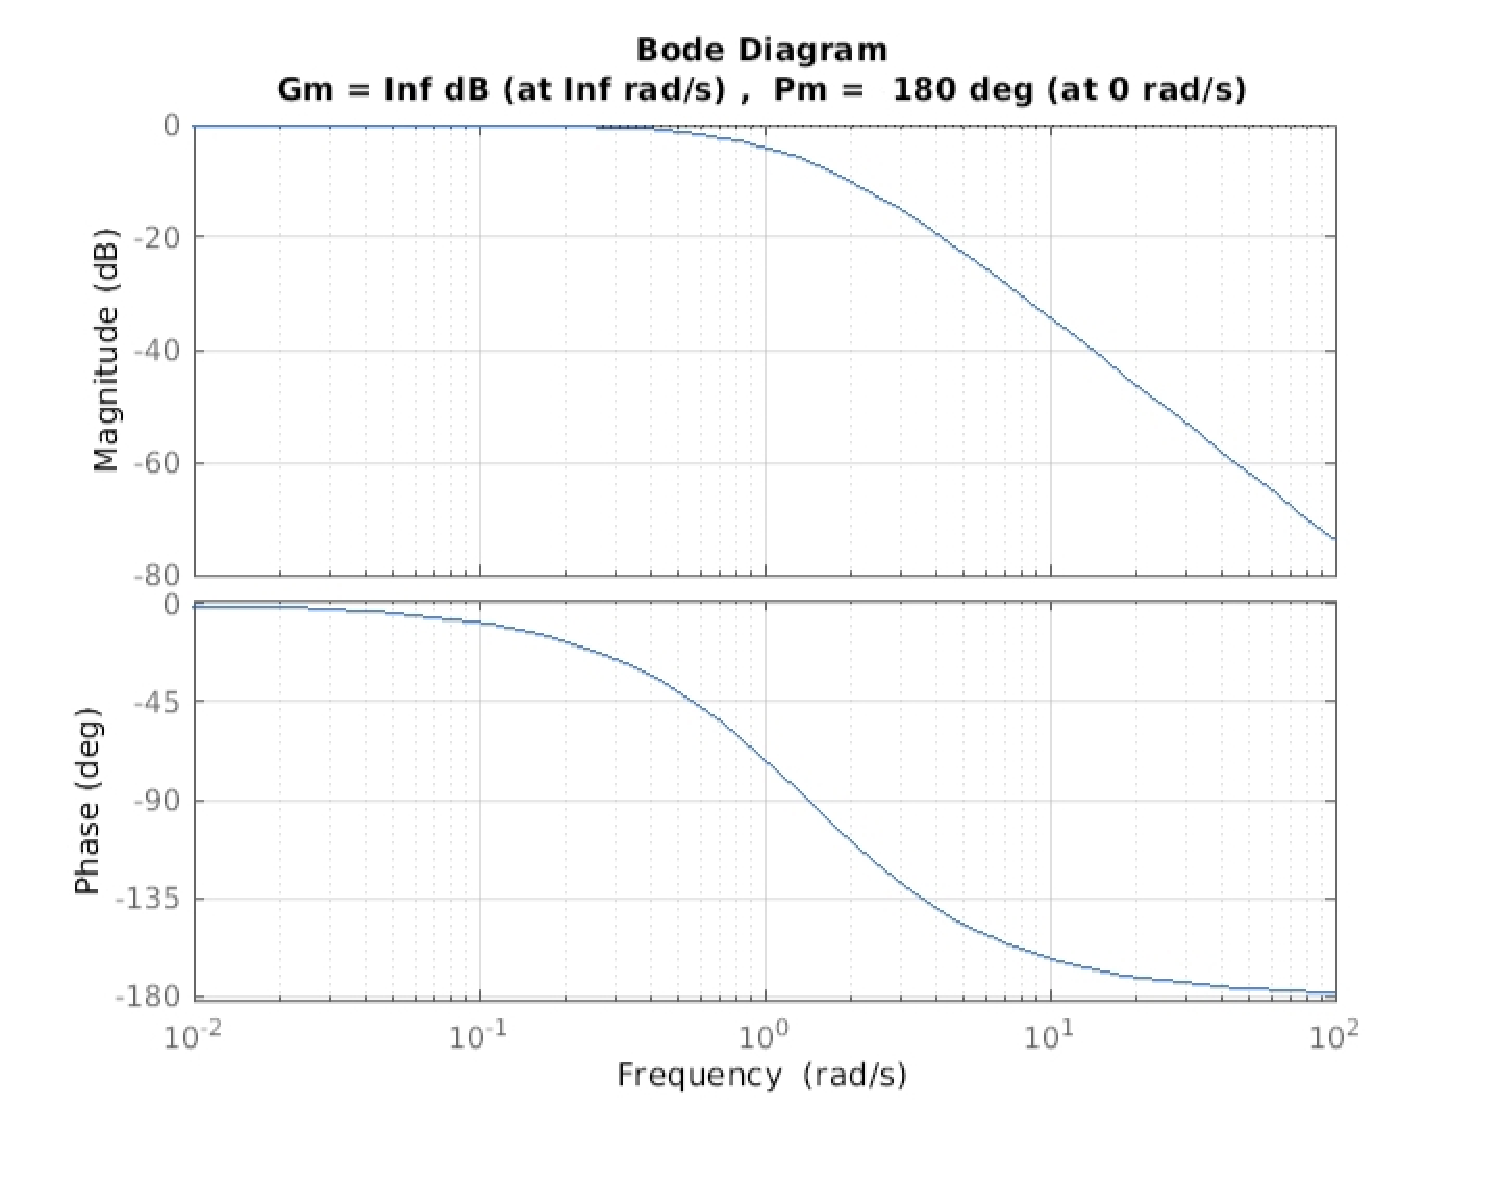
\includegraphics[scale=0.39]{./figs/bode.eps}
\end{figure}
}
\end{frame}
\\\\\\\\
\begin{frame}{Question-17 }
 Consider the linear system \emph{$\dot{x}$} =
\begin{bmatrix}
-1 & 0\\
0 & -2
\end{bmatrix}x , with initial condition\\x(0) =
\begin{bmatrix}
1\\
1
\end{bmatrix}. The solution x(t) for this system is: \\
\vspace{7mm}

(A) x(t) =
\begin{bmatrix}
e^{-t} & te^{-2t}\\
0 & e^{-2t}
\end{bmatrix}
\begin{bmatrix}
1\\
1
\end{bmatrix} 
\\
(B) x(t) =
\begin{bmatrix}
e^{-t} & 0\\
0 & e^{2t}
\end{bmatrix}
\begin{bmatrix}
1\\
1
\end{bmatrix}
\\
\vspace{3mm}
(C) x(t) =
\begin{bmatrix}
e^{-t} & t^{2}e^{-2t}\\
0 & e^{-2t}
\end{bmatrix}
\begin{bmatrix}
1\\
1
\end{bmatrix} 
\\ 
(D) x(t) =
\begin{bmatrix}
e^{-t} & 0\\
0 & e^{-2t}
\end{bmatrix}
\begin{bmatrix}
1\\
1
\end{bmatrix}
\\


\end{frame}
\begin{frame}{Solution:- }
It is of the form \emph{$\dot{x}$ = Ax}. Therefore its solution is \\
\vspace{3mm}
\hspace{30 mm}x(t) = e^{At}x(0)\\
$e^{At}$ is my state transition matrix 
and is equal to\\
\hspace{30mm}
$\mathcal{L}$^{-1}$[sI - A]^{-1}$ \hspace{7mm} (derivation in last slide)\\
\hspace{5mm}
A = 
\begin{bmatrix}
-1 & 0\\
0 & -2
\end{bmatrix} \hspace{20mm}
$\therefore$ [sI - A] = 
\begin{bmatrix}
s+1 & 0\\
0 & s+2
\end{bmatrix}\\
\vspace{5mm}
\hspace{5mm}
\rightarrow Adj(sI -A) =
\begin{bmatrix}
s+2 & 0\\
0 & s+1
\end{bmatrix}\\
\vspace{5mm}
\hspace{5mm}
\rightarrow det(sI -A) = (s+1)(s+2)
\end{frame}
\begin{frame}{}
%\begin{center}
\hspace{5mm}
$\therefore$ [sI - A]^{-1} = \frac{Adj(A)}{det(A)} = 
\begin{bmatrix}
\frac{1}{s+1} & 0\\
0 & \frac{1}{s+2}
\end{bmatrix} \\
\vspace{5mm} \hspace{5mm}
e^{At} = 
\begin{bmatrix}
\mathcal{L}^{-1}[\frac{1}{s+1}] & 0\\
0 & \mathcal{L}^{-1}[\frac{1}{s+2}]
\end{bmatrix} \\
\vspace{5mm} \hspace{5mm}
e^{At} = 
\begin{bmatrix}
e^{-t} & 0\\
0 & e^{-2t}
\end{bmatrix} \\
\vspace{5mm} \hspace{5mm}
\therefore x(t) = e^{At} x(0)   =    
\begin{bmatrix}
e^{-t} & 0\\
0 & e^{-2t}
\end{bmatrix}
\begin{bmatrix}
1\\
1
\end{bmatrix}
\\
\vspace{5mm} \hspace{20mm}
\rightarrow \emph{OPTION (D)}
%\end{center}
\end{frame}
\begin{frame}{}
Derivation of state transition matrix
\hspace{25mm}
\rightarrow \dot{x} = Ax \\
\vspace{5mm} \hspace{25mm}
Taking Laplacian\\
\vspace{5mm} \hspace{20mm}
\rightarrow S.X(s) -x(0) = AX(s)\\
\vspace{5mm} \hspace{20mm}
\therefore X(s) = [SI -A]^{-1}x(0)\\
\vspace{5mm} \hspace{20mm}
X(t) = $\mathcal{L}$^{-1} [SI -A]^{-1}x(0)\\
\vspace{5mm} \hspace{20mm}
\rightarrow Here,  \mathcal{L}^{-1}$[SI -A]^{-1}$  is called the state transition matrix
\\\\
\end{frame}
\\\\\\\\
\begin{frame}{Question.18 }
Consider a standard negative feedback configuration with 
G(s)=$\frac{1}{(s+1)(s+2)}$ and H(s)=$\frac{s+\alpha}{s}$
the closed loop system to have poles on the imaginary axis, the value of  $\alpha$ should be equal to (up to one
decimal place
\end{frame}
\\\\
\begin{frame}{Solution:- }
\begin{center}
    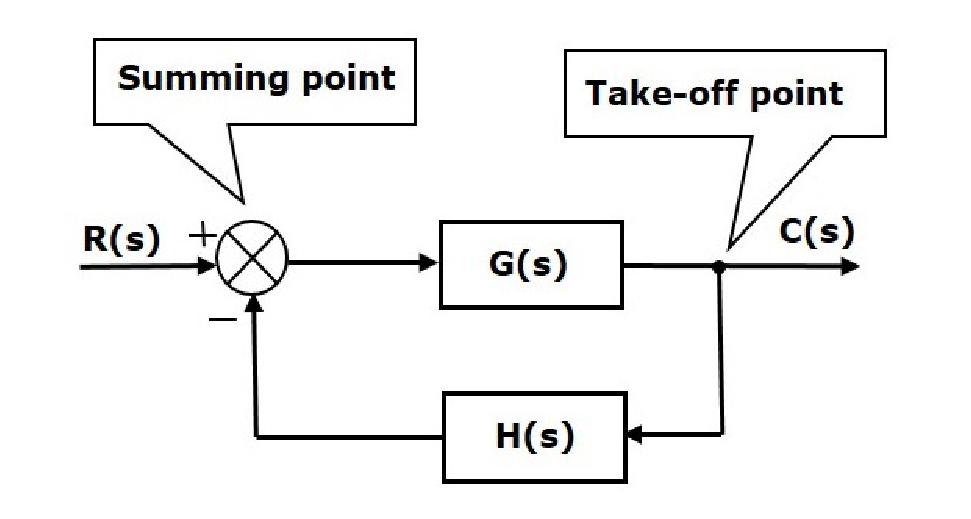
\includegraphics[width=6cm,0.5]{./figs/basic_block_diagram.eps}
\end{center}
\end{frame}
\begin{frame}{}
 Negative feedback system with G(s)=$\frac{1}{(s+1)(s+2)}$ ,H(s)=$\frac{s+\alpha}{s}$
 \\\\
\\ transfer function for negative feedback system  $\frac{C(s)}{R(s)}$=$\frac{G(s)}{1+G(s)H(s)}$
\\\\
 $\frac{G(s)}{1+G(s)H(s)}$=$\frac{\frac{1}{(s+1)(s+2)}}{1+\frac{1}{(s+1)(s+2)}\frac{s+\alpha}{s}}$ 
\\
 transfer function = $\frac{s}{(s^3 +3s^2+ 3s+ \alpha)}$ 
 \\
\end{frame}
\begin{frame}{}
we have to find value of $\alpha$ for which the poles of the system will be lying on imaginary axis.
 for determining the location of closed loop poles 
\\
        \polylongdiv{s^3+3s^2+3s}{}+ $\alpha$=0 
   \\

 \end{frame}
\begin{frame}{}

 Hence we can form the Routh’s array using characteristic polynomial  
 \\
 \hspace{3cm} P(s)=\polylongdiv{s^3+3s^2+3s}{}+ $\alpha$ \hfill \break
 
  \hspace{3cm} \polylongdiv{s^3}{} \hspace{1cm} 1\hspace{1cm} 3\hspace{1cm} 0 \hfill \break
  
  \hspace{3cm} \polylongdiv{s^2}{} \hspace{1cm} 3\hspace{1cm} \alpha\hspace{1cm} 0 \hfill\break
  
  \hspace{3cm} \polylongdiv{s^1}{} \hspace{1cm} \frac{(9-\alpha)}{3} \hspace{0.5cm}0\hspace{1cm}0
  
  \hspace{3cm} \polylongdiv{s^0}{}\hspace{1cm} \alpha\hspace{1cm} \hspace{0.5cm}0\hspace{1cm}0\hfill \break
  \end{frame}
\begin{frame}{}
  If closed loop poles will be lying on imaginary axis, then the system will be marginally stable and the
conditions is satisfied by Routh’s array, if any complete row (except last) become zero.
 Having seen the first column of Routh’s array, poles will on imaginary axis, when \\
 
 \hspace{3cm}     $\frac{(9-\alpha)}{3}=0 \hfill \break
  
  \hspace{3cm}   Hence, \alpha=9
  
  \hspace{0.5cm} now put $\alpha$=9 in characteristic equation 
  now characteristic equation is P(s)=\polylongdiv{s^3+3s^2+3s+9}{}\hfill\break
  
  \hspace{1cm} poles are s= -3,j$\sqrt{3}$ ,-j$\sqrt{3}
  
\\\\\\\  
\end{frame}
\\\\
\begin{frame}{Question-19 }
Unit Step response of a linear time invariant (LTI) system is given by $y(t) = (1 - e^{-2t})u(t)$. Assuming zero initial condition, the transfer function of the system is 

\vskip 1cm

\begin{itemize}
\item (A) $\frac{1}{s+1}$
\item (B) $\frac{2}{(s+1)(s+2)}$
\item (C) $\frac{1}{s+2}$
\item (D) $\frac{2}{s+2}$
\end{itemize}

\end{frame}

\begin{frame}{Solution:- }
Unit step response in time domain is
\[y(t) = (1 - e^{-2t})u(t)\]
\vskip 0.5cm
We can convert this step response into s-domain using the Laplace Transform
\[Y(s) = \mathcal{L}(y(t))\]
\[where \quad \mathcal{L}(y(t))= \int_{-\infty}^{\infty} y(t)e^{-st} dt\]

\end{frame}

\begin{frame}{}
From the properties of Laplace Transform we know that:
\vskip 0.5cm
\begin{itemize}
\item $\mathcal{L}(ax(t) + by(t)) = a\mathcal{L}(x(t)) + b\mathcal{L}(y(t))$
\vskip 0.5cm
\item $\mathcal{L}(u(t)) = \frac{1}{s}$\\*
\vskip 0.2cm
where
\[   
u(t) = 
     \begin{cases}
       \text{1} &\quad\text{if t $\ge$ 0}\\
       \text{0} &\quad\text{if t < 0} \\ 
     \end{cases}
\]

\vskip 0.5cm
\item $\mathcal{L}(e^{-at}u(t)) = \frac{1}{s + a}$
\end{itemize}

\end{frame}

\begin{frame}{}

$Y(s) = \mathcal{L}(y(t))$\\*
\vskip 0.3cm
$= \mathcal{L}(u(t) - e^{-2t}u(t))$\\*
\vskip 0.3cm
$= \mathcal{L}(u(t)) - \mathcal{L}(e^{-2t}u(t))$\\*
\vskip 0.3cm
$= \frac{1}{s} - \frac{1}{s+2}$\\*
\vskip 0.3cm
$= \frac{2}{s(s+2)}$\\*

\vskip 1cm
$x(t) = u(t)  \because  $Input is the Unit step function\\*
\vskip 0.3cm
$\implies X(s) = \frac{1}{s}$\\*

\end{frame}

\begin{frame}{}

The Transfer Function $H(s)$ is given by\\*
\vskip 0.3cm
$H(s) = \frac{Y(s)}{X(s)}$
$= \frac{\frac{2}{s(s+2)}}{\frac{1}{s}}$
$= \frac{2}{s+2}$
\vskip 1cm
Hence the Transfer Function $H(s)$ is $\frac{2}{s+2}$\\*
Option(D)
\end{frame}

\begin{frame}{}

\begin{figure}
  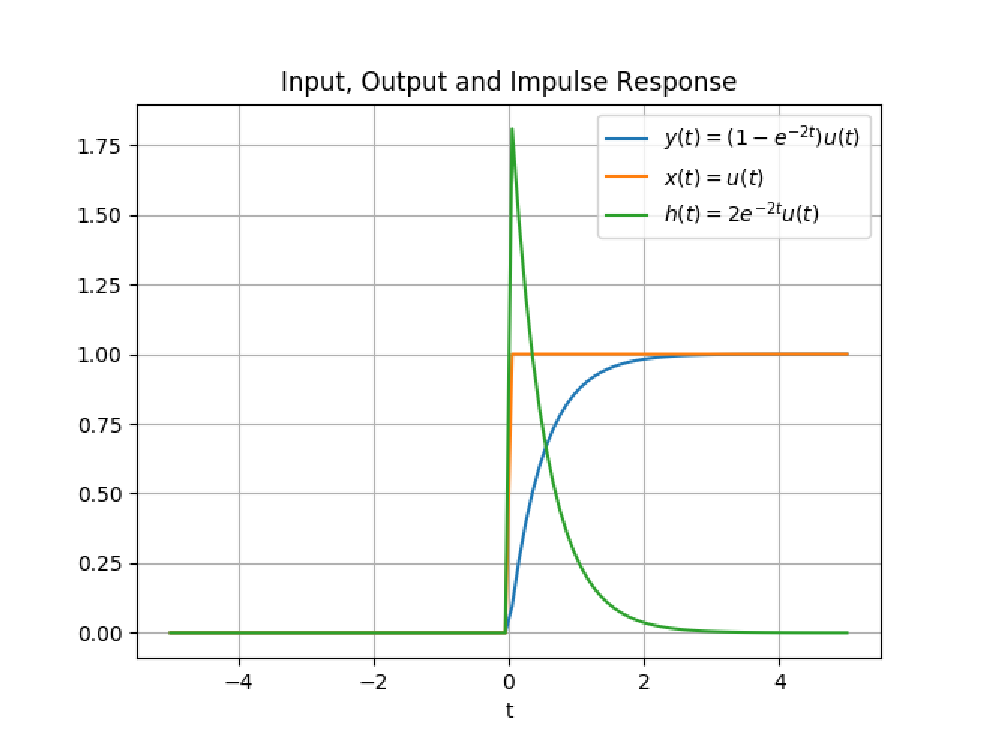
\includegraphics[width=\linewidth]{./figs/Plot_1.eps}
  \caption{All Functions Plot}
\end{figure}
\end{frame}
\\\\
\begin{frame}{Question-20 }
The Nyquist stability criterion and the Routh criterion both are powerful analysis tools for
determining the stability of feedback controllers. Identify which of the following statements
is FALSE:
\\
(A) Both the criteria provide information relative to the stable gain range of the system.
\\(B) The general shape of the Nyquist plot is readily obtained from the Bode magnitude plot
for all minimum-phase systems.
\\(C) The Routh criterion is not applicable in the condition of transport lag, which can be
readily handled by the Nyquist criterion.
\\ (D) The closed-loop frequency response for a unity feedback system cannot be obtained
from the Nyquist plot. 

\end{frame}
\begin{frame}{Solution:- }
\\
     The answer is option:(D)
\\ The closed-loop frequency response for a unity feedback system cannot be obtained from the Nyquist plot. 

\end{frame}

\begin{frame}{}
\\
 Option(A) Both the criteria provide information relative to the stable gain range of the system is true.
\\ Option(B) It's true because as in a minimum-phase system, Bode magnitude plot is enough to obtain a general
approximation of its Nyquist plot.

\end{frame}

\begin{frame}{}
\\    
     Option(C)  Routh criterion can be applied to any system to check the stability of a system but a transport lag
controller can only by explained using Nyquist Criterion.
\\
 Option(D)  We can obtain closed-loop frequency response for Unity Feedback system easily by substituting s
= jω, and draw the plot for different values of ω. Usually this is not done as it is not necessary as
OLTF is enough to comment on the stability. Thus, (D) is false.
\\   
\end{frame}
\\\\\\
\begin{frame}{Question-21 }
 The state equation and the output equation of a control system are given below :   
    \[\;\;\;\;\;\;\;\;\;\;\;\;\;\;\;\;\dot{X} =
  \left[ {\begin{array}{cc}
   -4 & -1.5 \\
   4 & 0 \\
  \end{array} }\right] X +
  \left[ {\begin{array}{cc}
  
      4   \\
      0 \\
  \end{array} }\right] U\]
  
    \[Y = 
 \left[ {\begin{array}{cc}
   1.5 & 0.625 \\
  \end{array} }\right] X \]
   
Then transfer function representation of the system is 
\vskip 0.8cm
\;\;\;\;(A) $\frac{(3s + 5)}{(s^2 + 4s + 6)}$ \; \;\; \;\;\;\;\;\;\;\;\;\;\;\;\;\;\;    (B) $\frac{(3s -1.875)}{(s^2 + 4s + 6)}$
\vskip 0.5cm
\;\;\;\;(C) $\frac{(4s + 1.5)}{(s^2 + 4s + 6)}$ \; \;\; \;\;\;\;\;\;\;\;\;\;\;\;\;\;\; (D) $\frac{(6s + 5)}{(s^2 + 4s + 6)}$
\vskip 0.4cm


\vskip 1cm

\end{frame}

\begin{frame}{Solution:- }
 From the given state space representation of the system, we can find matrices as
 \[
   A=
  \left[ {\begin{array}{cc}
   -4 & -1.5 \\
   4 & 0 \\
  \end{array} } \right] ,  
  B = \left[ {\begin{array}{cc}
  
      4   \\
      0 \\
  \end{array} }\right],                     C = \left[ {\begin{array}{cc}
   1.5 & 0.625 \\
  \end{array} }\right]\]
  when\[\;\dot{X} = AX + BU\]
  \[Y = CX + DU\]
  \\* where \; A,\,B,\,C,\,D \; are matrices 
  \\* Then\,the\, transfer\, function\, can\, be\, find\, using
  \[T(s) = C[(sI-A)^{-1}].B \,+ D\]
\end{frame}

\begin{frame}{}
\\*We can find the transfer function using

\[ T(s) = C[(sI - A)^{-1}].B \tag{$1$}\]

\[ \;\;\;\;\;\;\;\;\;\;\;(sI - A) = \left[ {\begin{array}{cc}
   s & 0 \\
   0 & s \\
  \end{array} } \right] - \left[ {\begin{array}{cc}
   -4 & -1.5 \\
   4 & 0 \\
  \end{array} } \right]\]
\[(sI - A) = \left[ {\begin{array}{cc}
   s + 4 & -1.5 \\
   -4 & s  \\
  \end{array} } \right] \tag{$2$}\]
   \vskip 0.01cm
\[ 
 \;\;\;\;\;\;\;\;\;\;\;\;\;\;\;\;\;\;\;\;|sI - A| \;\;\;= s(s+4) - (-4)\times (-1.5) \]
 \vskip 0.01cm
 
 \[\;\;\;\;\;\;\;\;\;\;\;\;\;\;\;= s^2 + 4s+ 6 \tag{$3$}\]
  \vskip 0.00001cm
 
 
  
\end{frame}
\begin{frame}{}
\[Adj[sI - A] = \left[ {\begin{array}{cc}
   s & -1.5 \\
   4 & s+4 \\
  \end{array} } \right]\]
  
  \vskip 0.1cm
\\*Hence
 \[[sI - A]^{-1} = \frac{Adj[sI - A]}{|sI - A|} = \left[ {\begin{array}{cc}
   \frac{s}{(s^2 + 4s + 6)} & \frac{-1.5}{(s^2 + 4s + 6)} \\
   \frac{4}{(s^2 + 4s + 6)} & \frac{(s + 4)}{(s^2 + 4s + 6)} \\
  \end{array} } \right] \tag{$4$}\]
  \vskip 0.1cm
\[
  [sI - A]^{-1}.B = \left[ {\begin{array}{cc}
   \frac{s}{(s^2 + 4s + 6)} & \frac{-1.5}{(s^2 + 4s + 6)} \\
   \frac{4}{(s^2 + 4s + 6)} & \frac{(s + 4)}{(s^2 + 4s + 6)} \\
  \end{array} } \right]\left[ {\begin{array}{cc}
  
      4   \\
      0 \\
  \end{array} }\right] \tag{$5$}
  \]
  \vskip 0.1cm
\dot{.\hspace{.095in}.}\hspace{.5in}
\vskip 0.1cm

\end{frame}
\begin{frame}{}
\[
\dot{.\hspace{.095in}.}\hspace{.5in} [sI - A]^{-1}.B =  \left[ {\begin{array}{cc}
   \frac{2s}{(s^2 + 4s + 6)} \\
   \frac{8}{(s^2 + 4s + 6)} \\
  \end{array} } \right] \tag{$6$}\]
 \vskip 0.1cm 
 Substituting\, values\, of\, [sI - A]^{-1}.B\, and\, C\, in\, equation\, (1)
\vskip 0.1cm
\[ T(s) = \left[ {\begin{array}{cc}
   1.5 & 0.625 \\
  \end{array} }\right]\left[ {\begin{array}{cc}
   \frac{2s}{(s^2 + 4s + 6)} \\
   \frac{8}{(s^2 + 4s + 6)} \\
  \end{array} } \right] \tag{$7$}
\]

\end{frame}
\begin{frame}{}
\[
 T(s) = \left[ {\begin{array}{cc}
   \frac{3s}{(s^2 + 4s + 6)} + \frac{5}{(s^2 + 4s + 6)} \\

  \end{array} } \right]
\]\\
\vskip 0.1cm

 the\,transfer\, function\, representation\, of\, the\, system\, is 
\vskip 0.5cm
\\
\[  T(s) = \left[ {\begin{array}{cc}
   \frac{3s + 5}{(s^2 + 4s + 6)} 
  \end{array} } \right]
\]
\end{frame}
\\\\\\\\
\begin{frame}{Question-22 }
For a unity feedback control system with the forward path transfer function
    $${G(s)} = \frac{k}{s(s+2)}$$
\\The peak resonant magnitude $M_{r}$ of the closed loop frequency is 2.The corresponding value of the gain K is

 \end{frame}
 \begin{frame}{Solution:- }
\\Given:
\\ For a unity feedback control system ${G(s)} = \frac{k}{s(s+2)}$ and resonant peak $M_{r}$=2
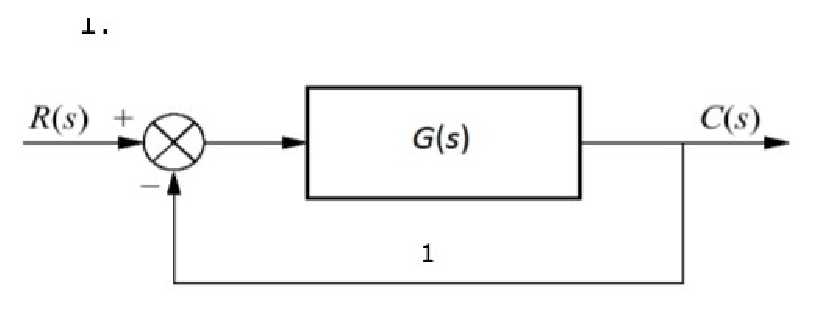
\includegraphics[width=.4\textwidth]{./figs/yeswanth(2).eps}
\\we can find its closed loop transfer function as,
\begin{equation}
    C(s)=[R(S)-H(S)C(S)]G(S) 
\end{equation}
\begin{equation}
    C(s)=R(S)G(S)-H(S)C(S)G(S)
\end{equation}
\begin{equation}
    C(S)+H(S)C(S)G(S)=R(S)G(S)
\end{equation}
\begin{equation}
    C(S)[1+G(S)H(S)]=R(S)G(S
\end{equation}
\begin{equation}
    \dfrac{C(s)}{R(s)}=T(s)=\dfrac{G(s)}{1+G(s)H(s)}
\end{equation}
\begin{equation}
T(s)=\dfrac{\dfrac{K}{s(s+2)}}{1+\dfrac{K}{s(s+2)*1}}=\dfrac{K}{s^2+2s+K}
\end{equation}
\end{frame}
\begin{frame}{}
\\standard equation of T(s) =\dfrac{\omega_{n}^2}{s^2+2S\xi^\omega_{n}+\omega_{n}^2}$
\\formula for resonant peak as $M_r=\dfrac{1}{2\xi(1-(\xi)^2)^\dfrac{1}{2}}$
\\
\\given resonant peak  $M_r=2$
\end{frame}
\\
$
\begin{equation}
   \dfrac{DC Gain}{2\xi(1-(\xi)^2)^\dfrac{1}{2}}=2
\end{equation}
\\
   \\here DC gain is 1 
\\squaring on both sides
\\16\xi^2(\xi^2-1)=1
\\$putting$ \xi^2=x
\\ \begin{equation}
    16x^2-16x+1=0
\end{equation}
\begin{equation}
    x=\xi^2=\dfrac{2-\sqrt{3}}{4}
\end{equation}
\begin{equation}
    x=\xi^2=\dfrac{2+\sqrt{3}}{4}
\end{equation}
\\ characteristic equation is $$s^2+2s+k$$
\\comparing it with standard equation we get $\omega_{n}$^2=k
\\2\xi^$\omega_{n}$=2
\\$$\xi=\dfrac{1}{\omega_{n}}=\dfrac{1}{k^\dfrac{1}{2}}$$
\\$$k=\dfrac{1}{\xi^2}=\dfrac{4}{2-\sqrt{3}} = 14.92$$
\end{frame}

\begin{frame}{Question-23 }
 The figure below shows the Bode magnitude and phase plots of a stable transfer function
    \begin{equation}    % <--- deleted empty lines
            G(s) = \frac{n_0}{s^3 + d_2 s^2 + d_1 s + d}
            \centering
    \end{equation}
    Consider the negative unity feedback configuration with gain \emph{k} in the feedforward path. The closed loop is stable for \emph{k} $\textless $ \emph{k_o} .\\  
    The maximum value of $\textit{{k_o}}$  is
\end{frame}

\begin{frame}{}

    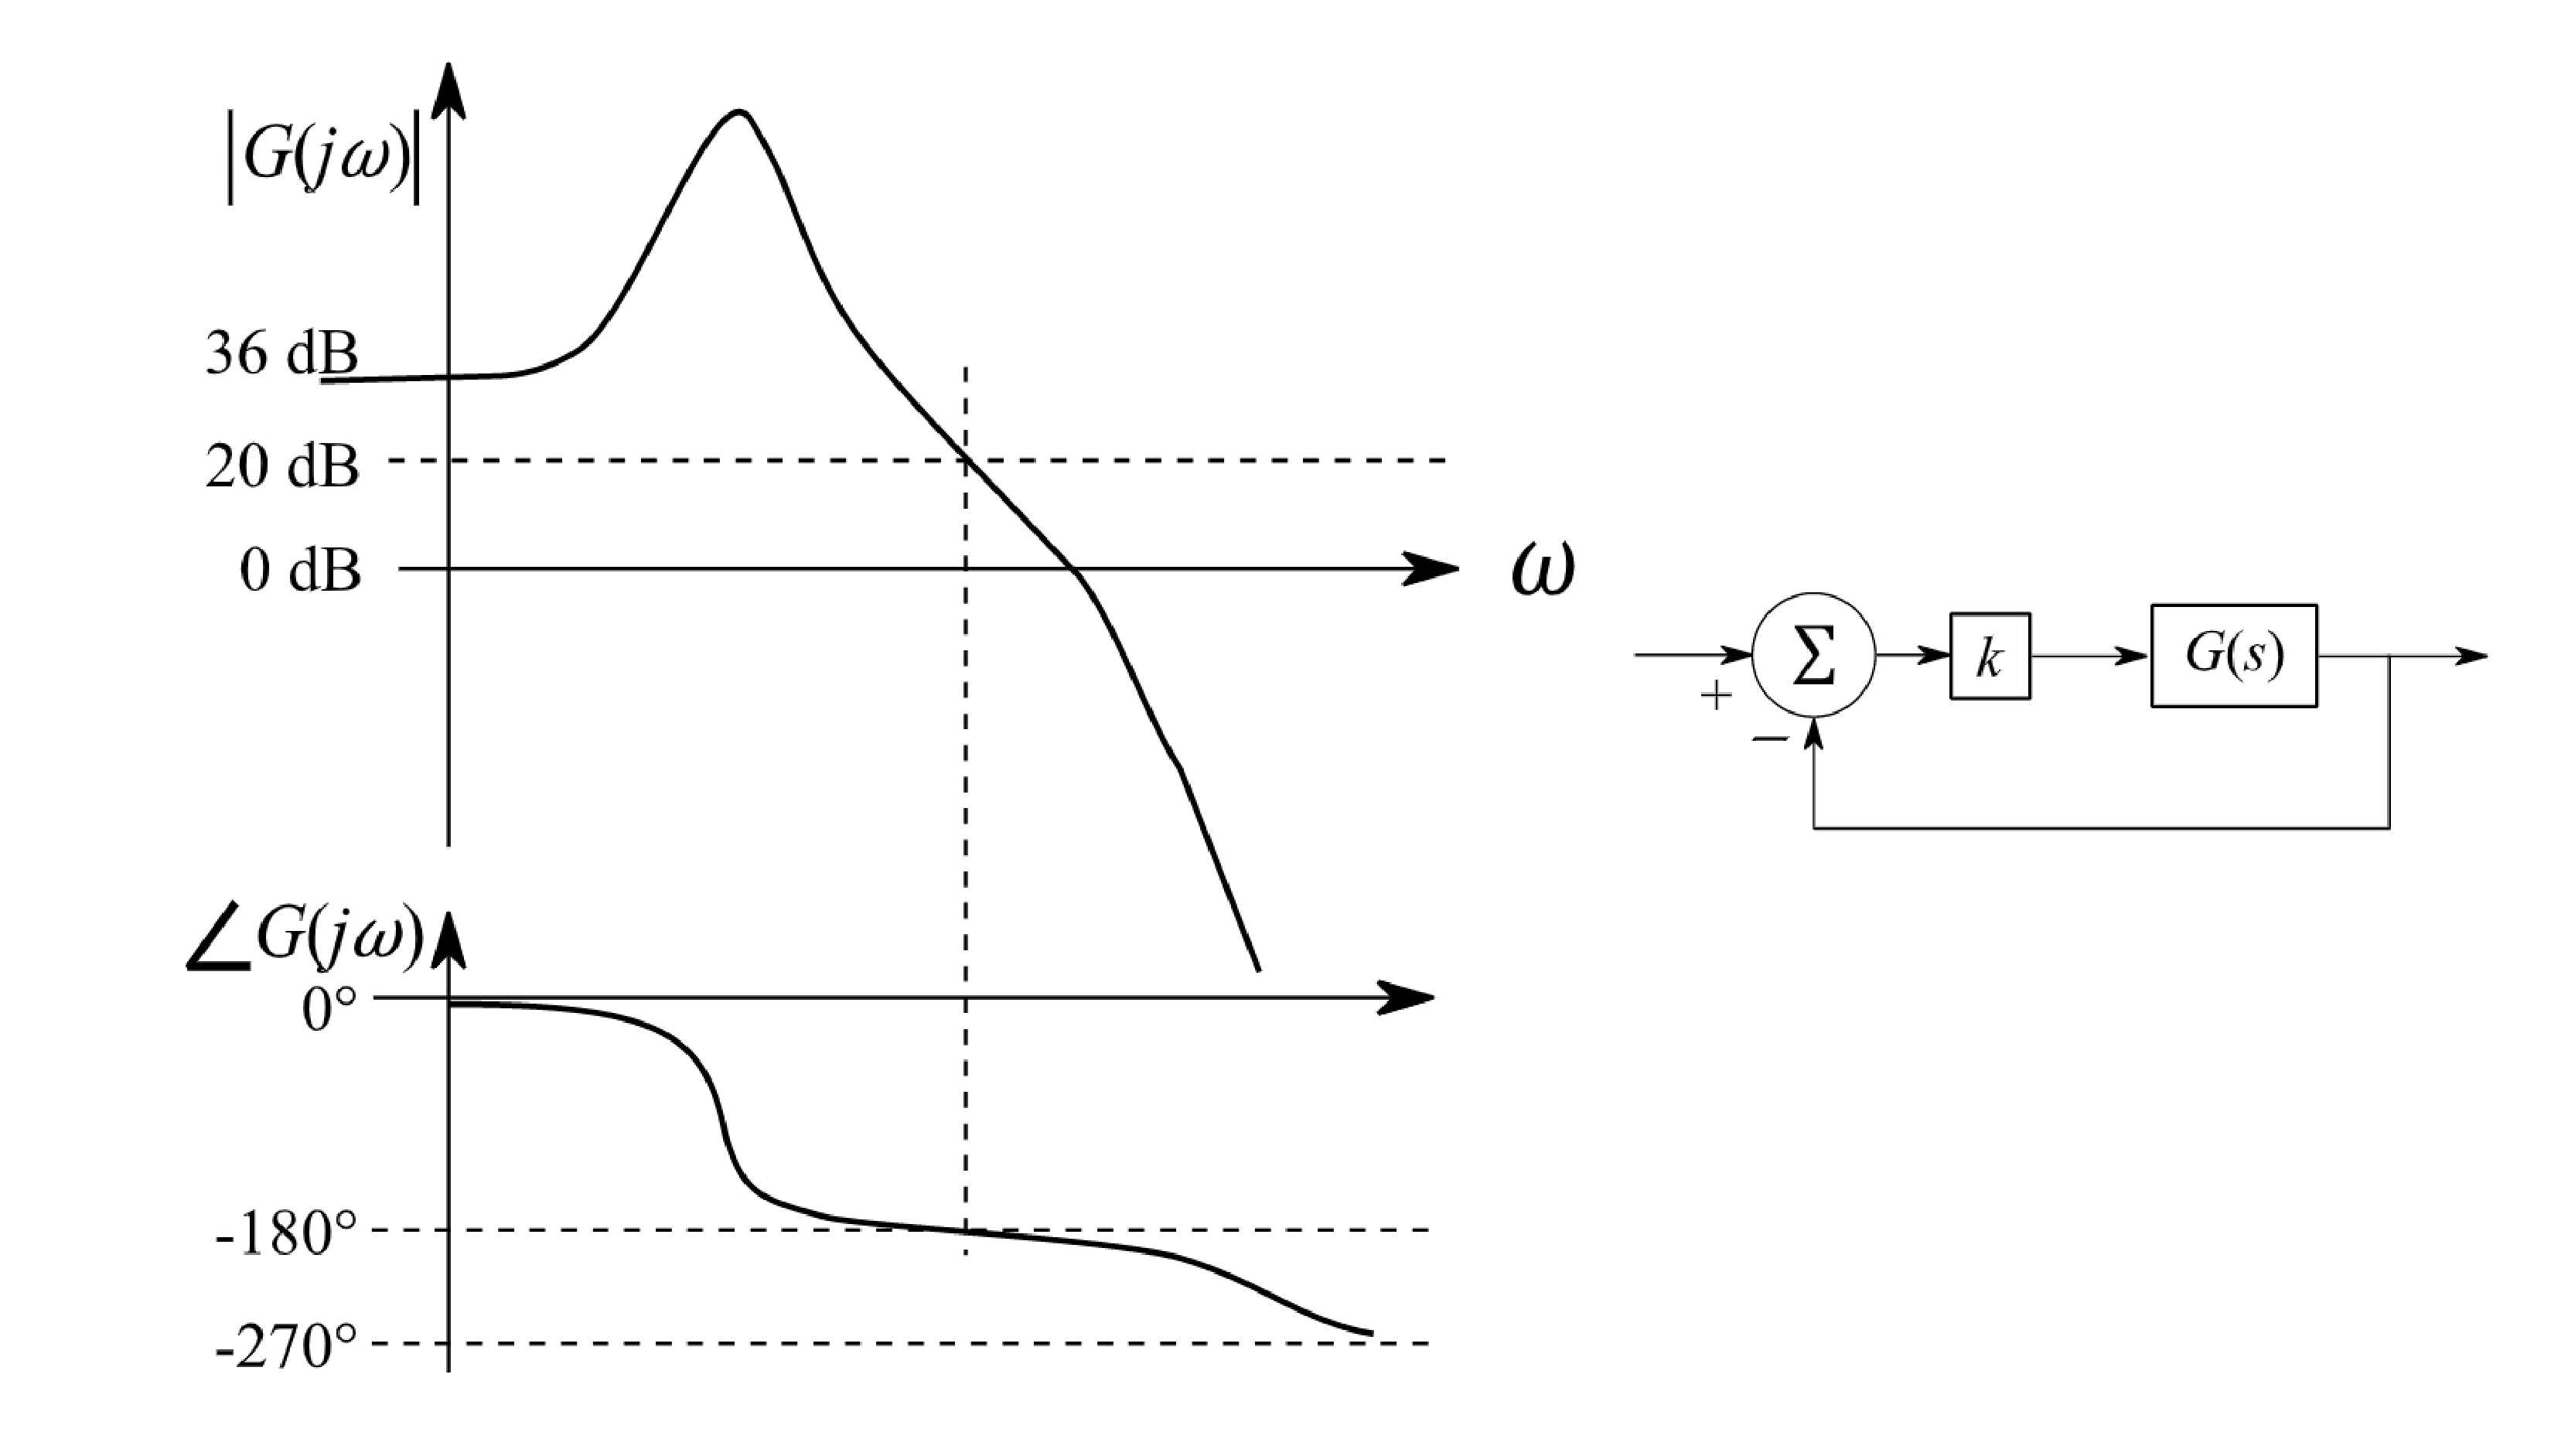
\includegraphics[scale = 0.15]{./figs/q42.eps}
    \centering

\end{frame}

\begin{frame}{Solution:- }
 \\ For a stable system, Gain margin at the phase cross-over frequency $\textgreater \ 0dB$.\\
Phase crossover frequency ($\omega_p_c)$}
   The phase crossover frequency is the frequency at which the phase angle first reaches -180 $\degree$.

   
   \begin{block}{}
This is the factor by which the gain must be multiplied at the phase crossover to have the value 1.
\\ The gain margin refers to the amount of gain, which can be increased or decreased without making the system unstable.
   \end{block}

\end{frame}

\begin{frame}{}
\begin{itemize}
\begin{center}
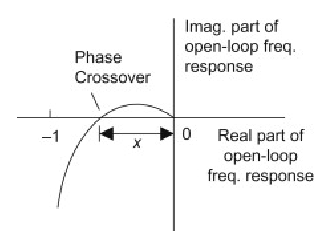
\includegraphics[scale = 1]{./figs/fig-1.eps}
\end{center}
\item The above shows nyquist plot of a stable transfer function.
\item The phase crossover frequency is the frequency at which the phase angle first reaches -180\degree and thus is the point where the Nyquist plot crosses the real axis.
\end{itemize}
\end{frame}

\begin{frame}{}

The gain margin is defined as \begin{equation*}
    K_g = \frac{1}{|G(j\omega)|}
\end{equation*} at the frequency at which the phase angle is -180\degree. 

In terms of decibels: 
 \begin{equation*}
    K_g dB = -20log(|G(j\omega)|) dB
\end{equation*}
    
\end{frame}

\begin{frame}{}
\begin{center}
    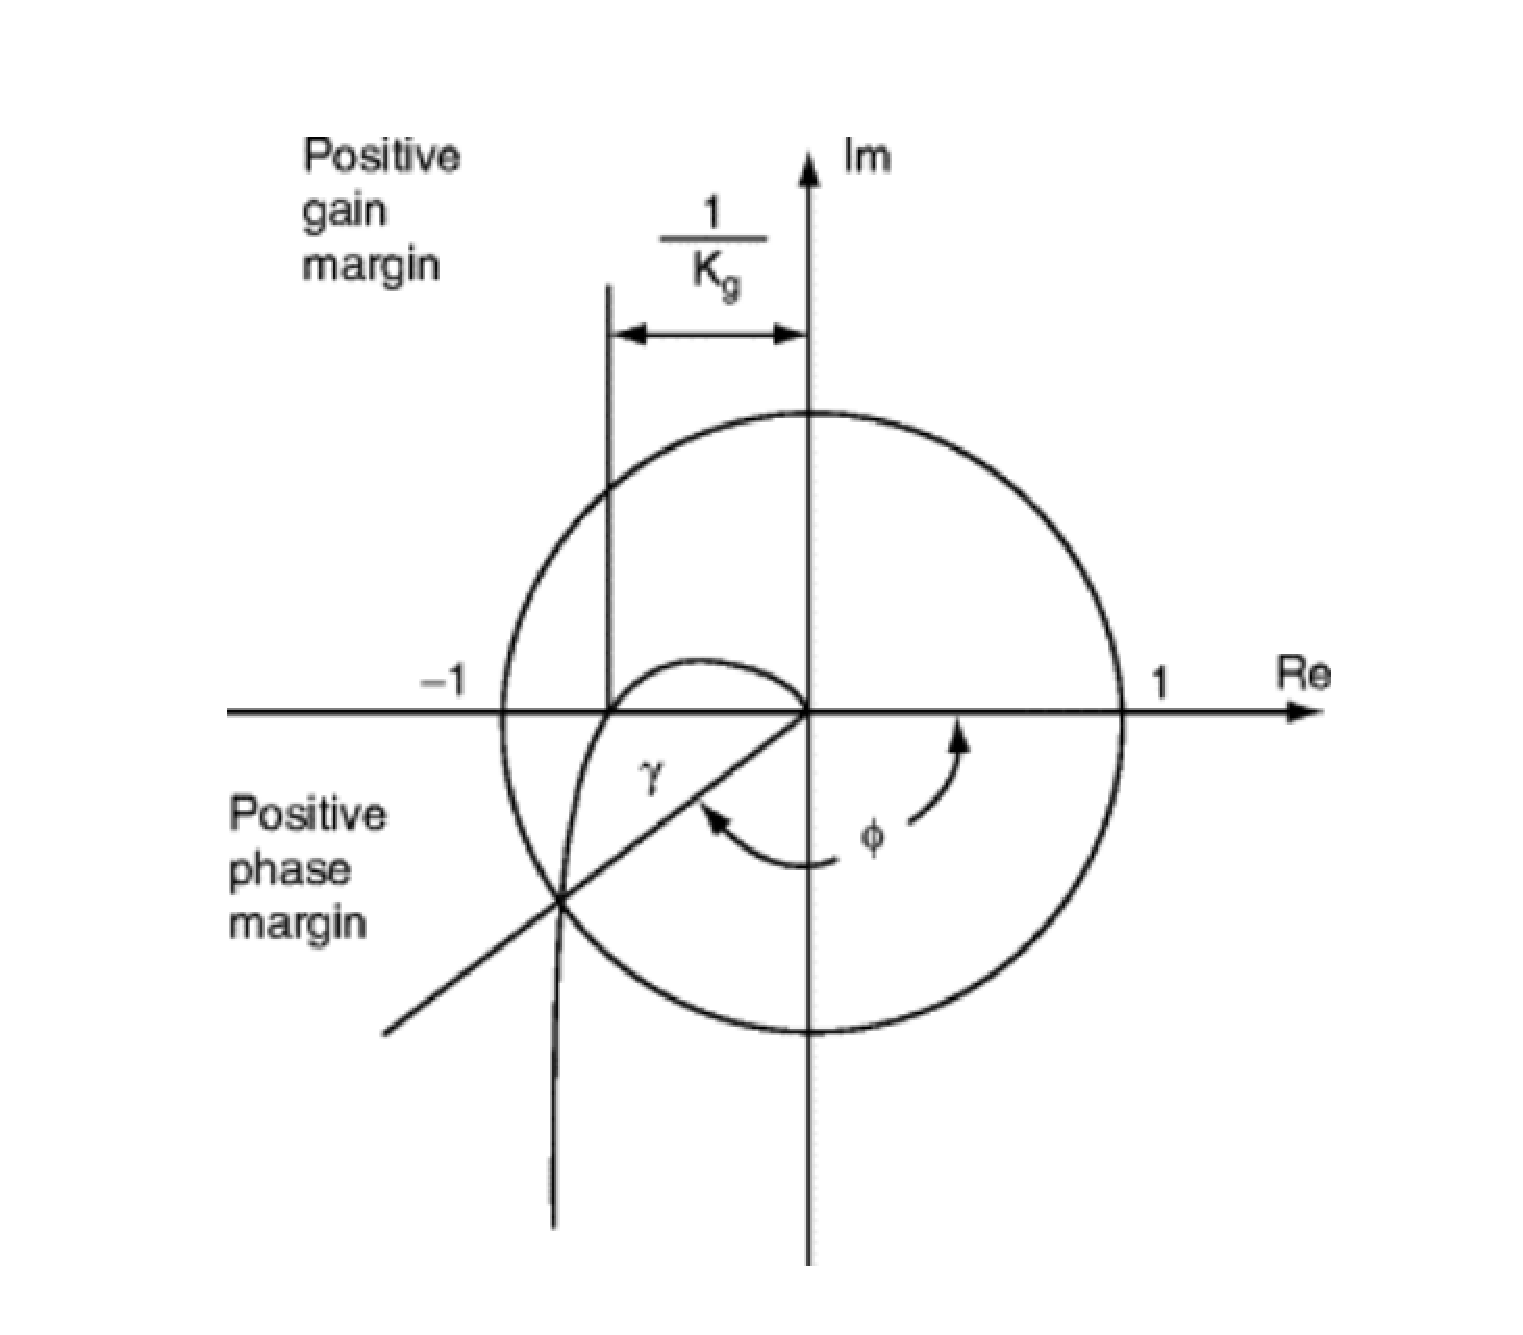
\includegraphics[scale = 0.25]{./figs/fig-2.eps}
\end{center}
\end{frame}

\begin{frame}{}
\begin{center}
    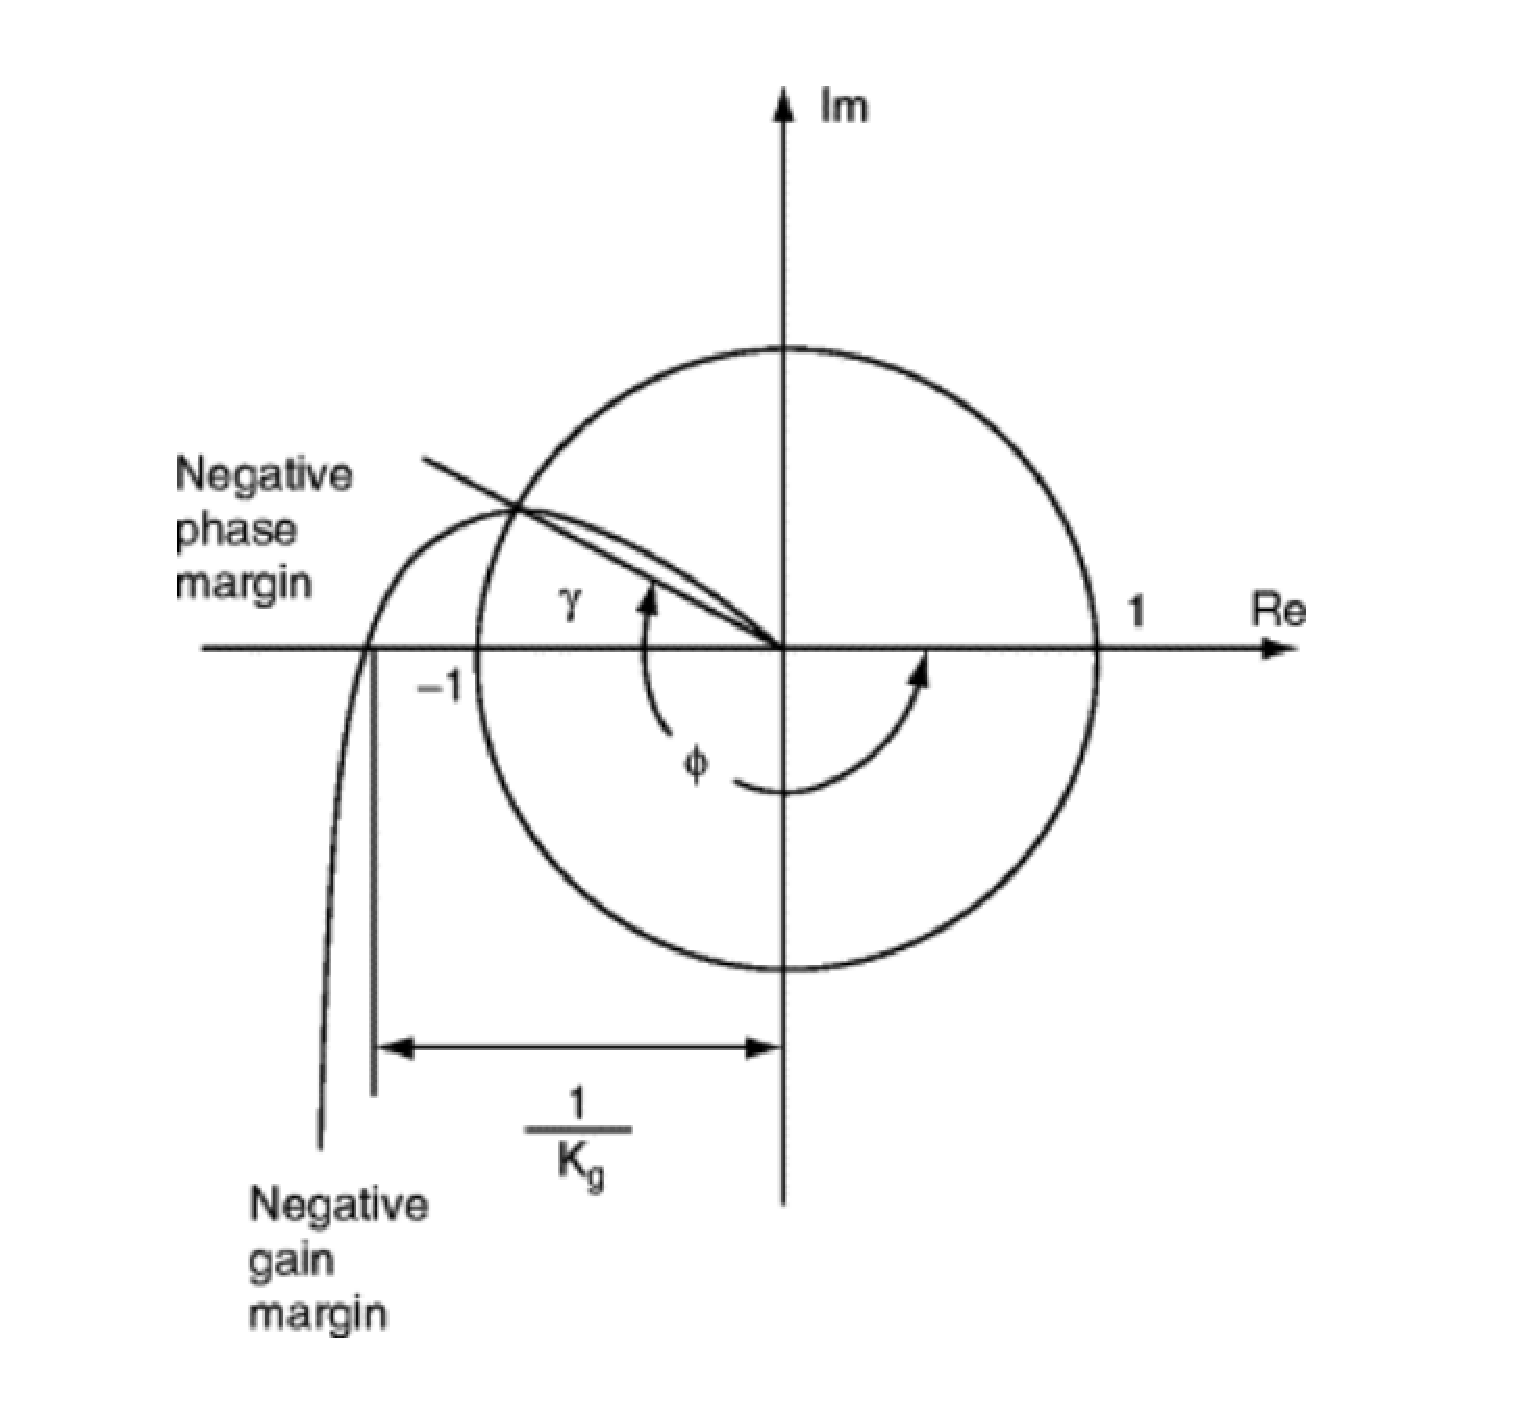
\includegraphics[scale = 0.25]{./figs/fig-3.eps}
\end{center}
\end{frame}


\begin{frame}{}
\par
For a stable system, Gain margin at the phase cross-over frequency \textgreater \ 1.

G(s) is cascaded with k, so,
\begin{equation*}
        G_1(s) = kG(s) \\
\end{equation*}
\begin{equation*}
        K_g = \frac{1}{|G_1(j\omega_p_c)|} \textgreater 1\\
\end{equation*}
\begin{equation*}
       \implies K_g_(_d_B_) = -20log(|G_1(j\omega_p_c)|) \textgreater \ 0dB
\end{equation*}



\end{frame}

\begin{frame}{}
\begin{equation*}
    \implies  -20log(|G(j\omega_p_c)k|) \textgreater \ 0dB
\end{equation*}

\begin{equation*}
    \implies  -20 - 20log(|k|) \textgreater \ 0dB
\end{equation*}

\begin{equation*}
   \implies 20log(k) \ \textless \ -20
\end{equation*}

\begin{equation*}
    \implies k \ \textless \ 10^-^1
\end{equation*}

\begin{equation*}
    \implies k_m_a_x = 0.1
\end{equation*}

\therefore k_o = 0.1
\\\\
\end{frame}
\\\\
\begin{frame}{Question-24 }
  \Q. Consider the state space realization : \vspace{2mm}\\
 $$\left[\begin{array}{l}
\dot{x_{1}(t)} \\
\dot{x_{2}(t)}
\end{array}\right]=\left[\begin{array}{cc}
{0} & {0} \\
{0} & {-9}
\end{array}\right]\left[\begin{array}{l}
{x_{1}(t)} \\
{x_{2}(t)}
\end{array}\right]+\left[\begin{array}{c}
{0} \\
{45}
\end{array}\right] u(t)$$ \smallskip  \\
with the initial conditions $$\left[\begin{array}{l}
{x_{1}(0)} \\
{x_{2}(0)}
\end{array}\right]=\left[\begin{array}{l}
{0} \\
{0}
\end{array}\right] $$, where u(t) denotes unit step function  \vspace{2mm} \\
\textbf { The value of } \textbf{\lim _{t \rightarrow \infty}|\sqrt{x_{1}^{2}(t)+x_{2}^{2}(t)}|} \textbf { is ? }

\end{frame}


\begin{frame}{Solution:- }
\textbf{State Space Reprensentation} : \text{A state-space representation is a mathematical}\\ model of a physical
system as a set of input, output\\ and state variables related by first-order differential equations.
\\\textbf{For Linear systems : }
\\$$\dot{\mathbf{x}}(t)=A(t) \mathbf{x}(t)+B(t) \mathbf{u}(t)$$
\\ where $\dot{\mathbf{x}}(t):=\frac{\mathrm{d}}{\mathrm{d} t} \mathbf{x}(t)$
\\$$\mathscr{L}\{x(t)\}=X(s)$$
\\$$\mathscr{L}\{\dot{x(t)}\}=sX(s) - x(0)$$
%\\$$\mathscr{L}\\{dot{x(t)\}=X(s)$$
\end{frame}
 
\begin{frame}{}
\left[\begin{array}{l}
\dot{{x_{1}(t)}} \\
\dot{{x_{2}(t)}}
\end{array}\right]=\left[\begin{array}{cc}
{0} & {0} \\
{0} & {-9}
\end{array}\right]\left[\begin{array}{l}
{x_{1}(t)} \\
{x_{2}(t)}
\end{array}\right]+\left[\begin{array}{c}
{0} \\
{45}
\end{array}\right] u(t) \vspace{5mm}\\
\text{By applying Laplace transform on both sides},\\
\text {we get}
\\  
$$
s X_{1}(s)-x_{1}(0)=0
$$
$X_{1}(s)=\frac{x_{1}(0)}{s}=0 \quad$     $\text \quad \because x_{1}(0)=0$
\\So, $\quad x_{1}(t)=0$\\
and $\quad s X_{2}(s)-x_{2}(0)=-9 X_{1}(s)+\frac{45}{s}$


\end{frame}

\begin{frame}{}
$$
\begin{aligned}
\text { Required value } &=\lim _{t \rightarrow \infty}|\sqrt{x_{1}^{2}(t)+x_{2}^{2}(t)}| \\
&=\left|\lim _{t \rightarrow \infty} x_{2}(t)\right|
\end{aligned}
$$

$\lim _{t \rightarrow \infty} x_{2}(t)=\lim _{s \rightarrow 0} s X_{2}(s)=\frac{45}{9}=5$ \vspace{5mm}\\
$\mathrm{So}$
Required value $=|5|=5$
\end{frame}

\begin{frame}{}
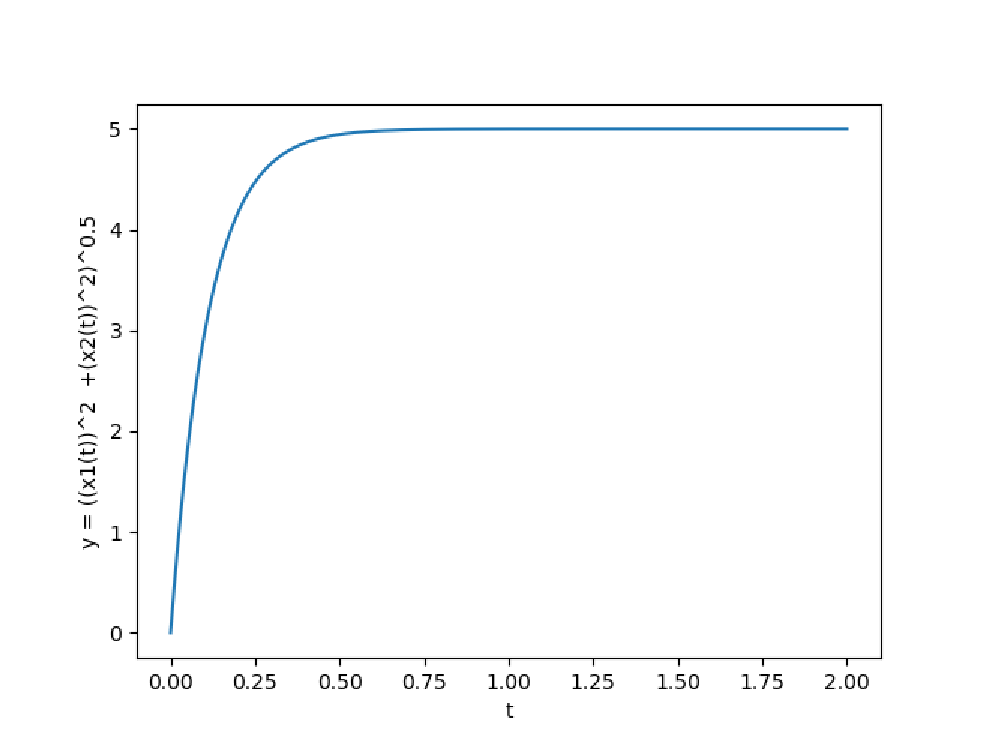
\includegraphics[scale=0.35]{./figs/gvv.eps}
\\\\\\
\end{frame}
\\\\\
\begin{frame}{Question-25 }
Consider the parallel combination of two LTI systems shown in the figure.
\begin{figure}[h]
    \centering
    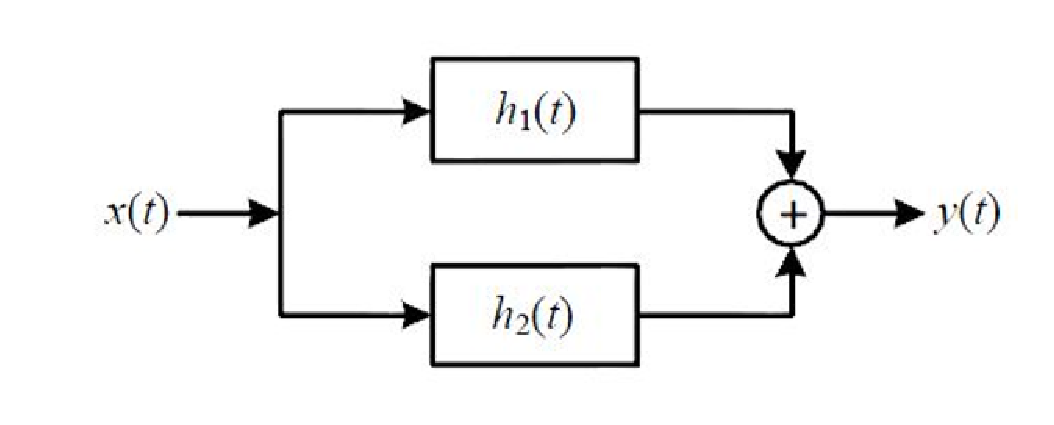
\includegraphics[width=3in]{./figs/fig-5.eps}
\end{figure}
The impulse response of the system are:
\\\qquad $h_1(t)=2\delta(t+2)-3\delta(t+1)$$
\\\qquad $h_2$(t)=$\delta(t-2)$
\\
If the input x(t) is a unit step \\ signal,then the energy of y(t) is ____ 
\end{block}   
\end{frame}
\\\\
\begin{frame}{Solution:- }
\\ Output of the system is found by convolving input x(t) with system's \\response h(t).
\\y(t)=x(t)*h(t)
\\Since $h_1$(t) and $h_2$(t) are connected in parallel the resultant system will be:
\\ h(t)=[$h_1$(t)+$h_2$(t)]
\end{frame}
\begin{frame}{}
\\ Given that x(t) is a unit step signal
\\$h_1$(t)+$h_2$(t)=$[2\delta(t+2)-3\delta(t+1)+\delta(t-2)]$
\\y(t)=2u(t+2)-3u(t+1)+u(t-2)
\begin{figure}[h]
    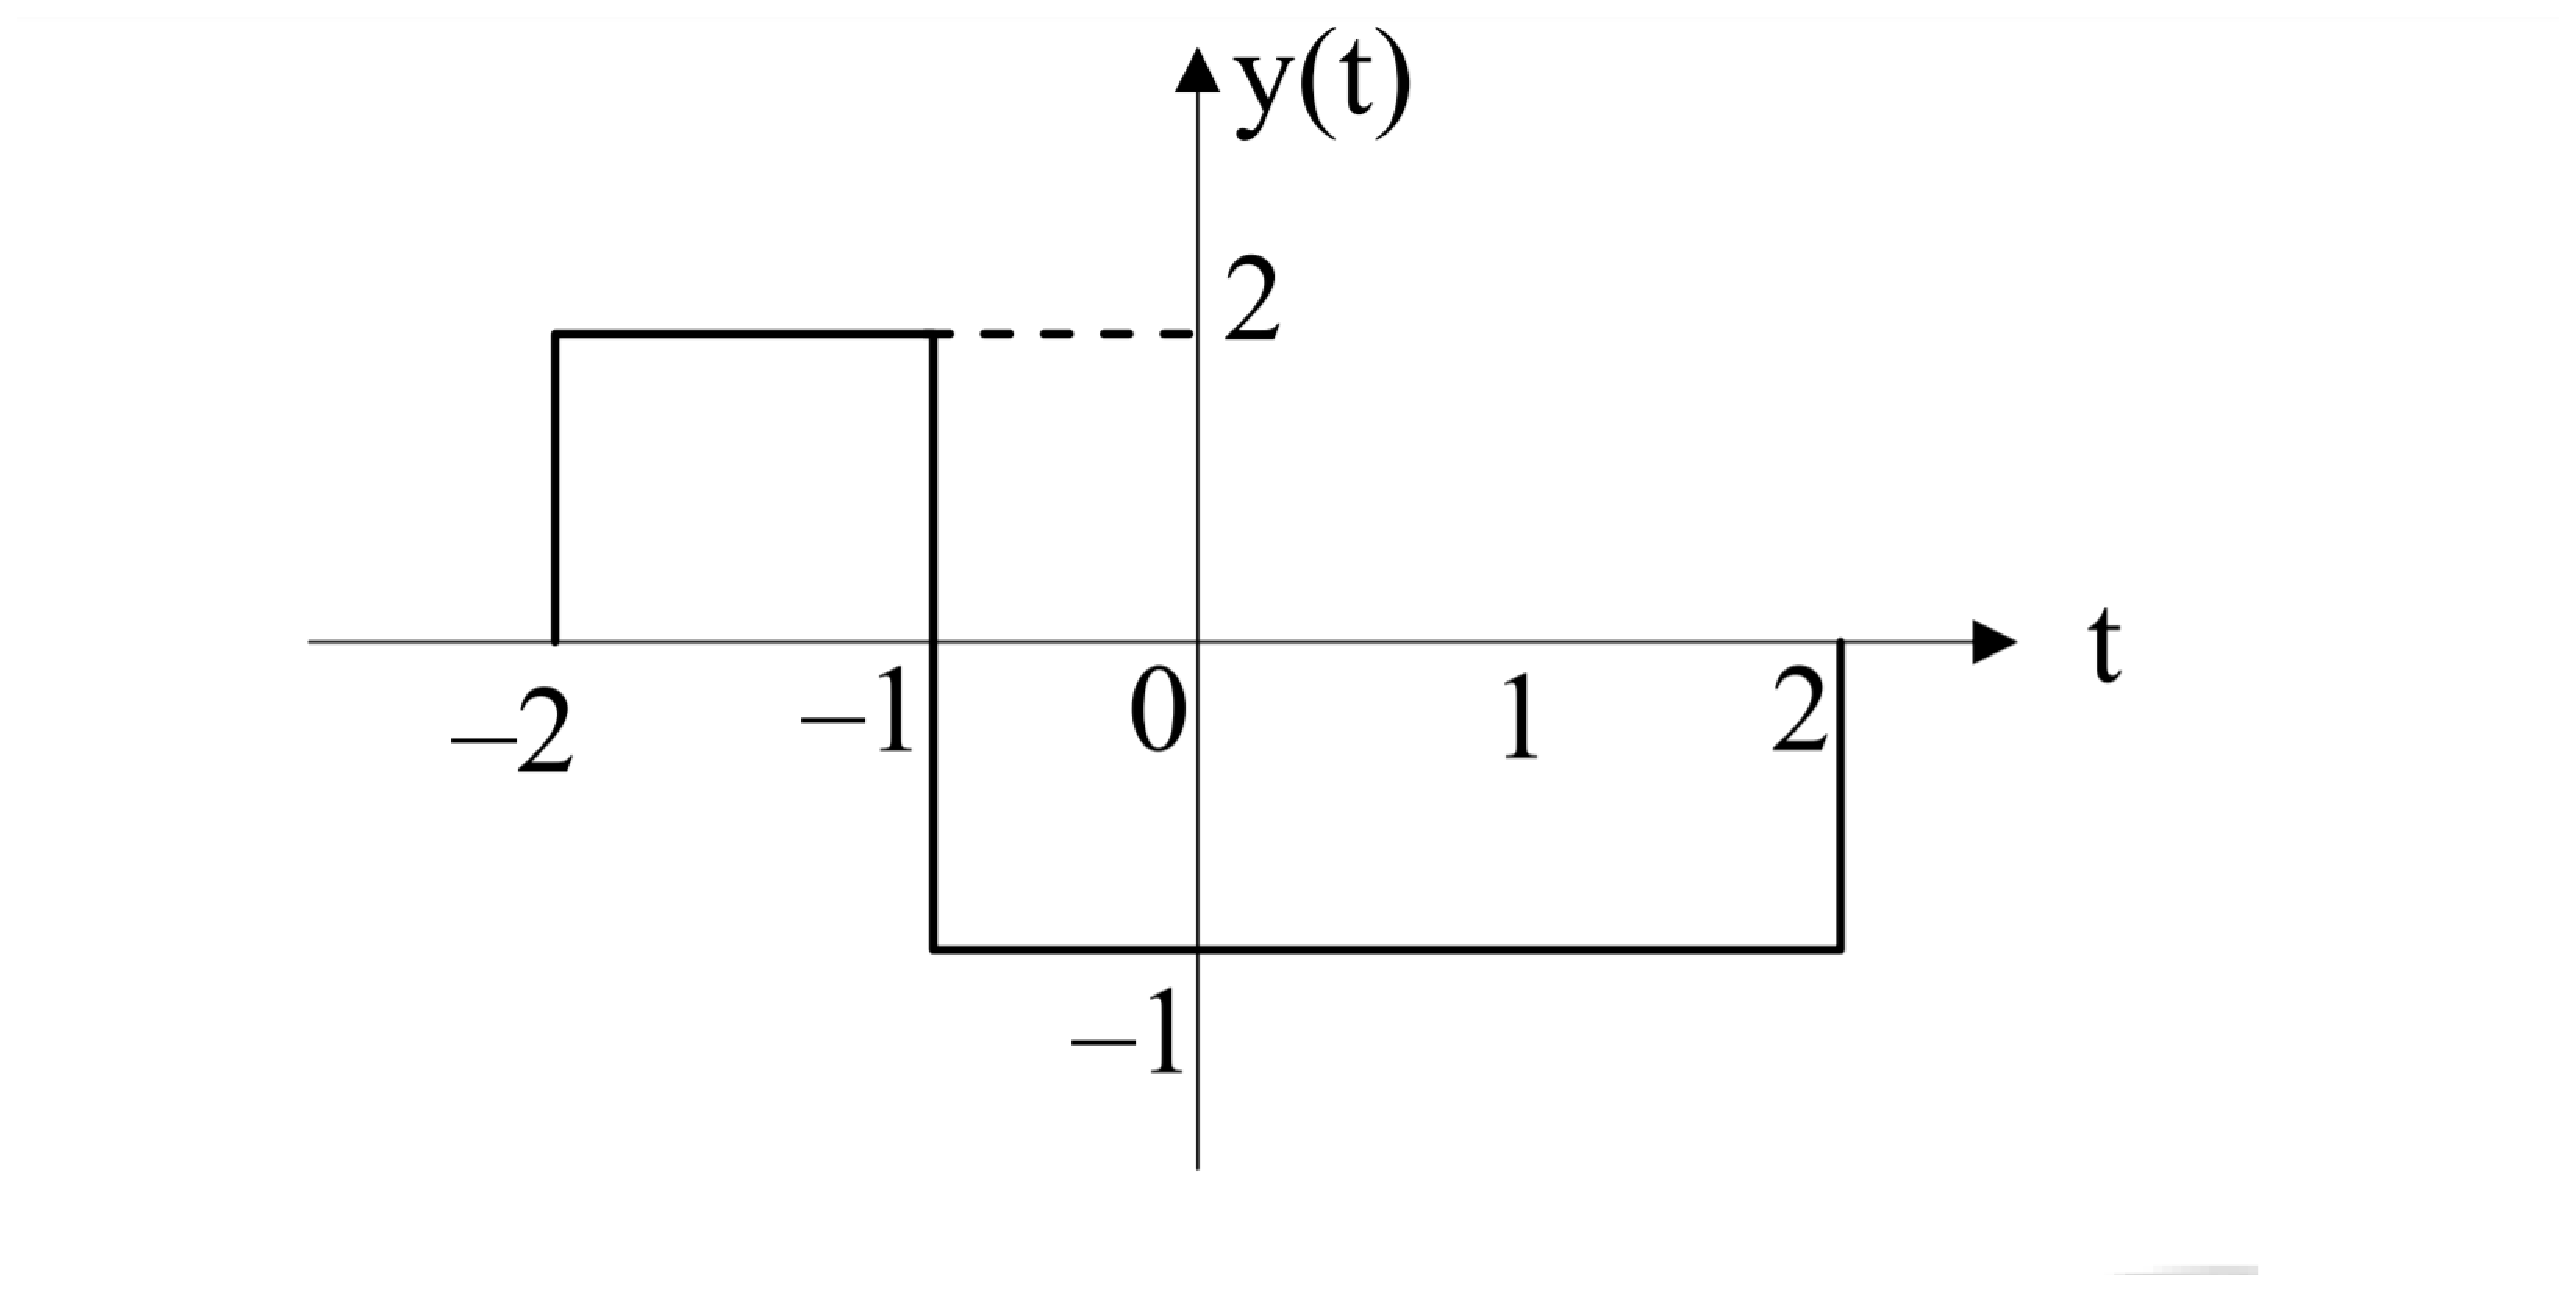
\includegraphics[scale=0.15]{./figs/16.eps}
\end{figure}
\\Energy of the given is
\\y(t)=$\int_{-2}^{-1} (2)^2 dx$ + $\int_{-1}^{2} (-1)^2 dx$
\\\quad\  =4[1]+1[3]
\\\quad\ =7  
\\\\\\
\end{frame}
\\\\
\begin{frame}{Question-26 }
A unity feedback control system is characterised by the open-loop transfer function\\
\begin{centre}
$$
 G(S) = \frac{2(s+1)}{s^3 + ks^2 + 2s +1}
$$
\end{centre}

the value of the k for which the system oscillates at 2 rad/s \\

\end{frame}
\begin{frame}{}
\begin{centre}


\tikzstyle{block} = [draw, fill=blue!20, rectangle, 
    minimum height=4em, minimum width=8em]
\tikzstyle{sum} = [draw, fill=blue!20, circle, node distance=1.5cm]
\tikzstyle{input} = [coordinate]
\tikzstyle{output} = [coordinate]
\tikzstyle{pinstyle} = [pin edge={to-,thin,black}]

% The block diagram code is probably more verbose than necessary
\begin{tikzpicture}[auto, node distance=3.5cm,>=latex']
    % We start by placing the blocks
    \node [input, name=input] {};
    \node [sum, right of=input] (sum) {};
    \node [block, right of=sum] (controller) {G(s)};
    \node [output, right of=controller] (output) {};
    \node [block, below of=controller] (measurements) {H(s) = 1};

    % Once the nodes are placed, connecting them is easy. 
    \draw [draw,->] (input) -- node {$R(s)\  +$} (sum);
    \draw [->] (sum) -- node {$E(s)$} (controller);
    \draw [->] (controller) -- node [name=y] {$Y(s)$}(output);
    \draw [->] (y) |- (measurements);
    \draw [->] (measurements) -| node[pos=0.99] {$-$} 
        node [near end] {$Y_m(s)$} (sum);
     
\end{tikzpicture}


\end{centre}

    
\end{frame}
\begin{frame}{Solution:- }
\begin{centre}
$$
E(s) = R(S) - Y_m(s)
$$
$$Y_m(s) = H(s)Y(s)$$
$$
 G(S) = \frac{Y(s)}{E(s)}
$$
$$
 G(S) = \frac{Y(s)}{R(s) - H(s)Y(s)}
$$
$$
 Gm(S) = \frac{Y(S)}{R(s)} = \frac{G(s)}{1 + H(s)G(s)}
$$


\end{centre}
\tikzstyle{block} = [draw, fill=blue!20, rectangle, 
    minimum height=3em, minimum width=6em]
%\tikzstyle{sum} = [draw, fill=blue!20, circle, node distance=1.5cm]
%\tikzstyle{input} = [coordinate]
%\tikzstyle{output} = [coordinate]
%\tikzstyle{pinstyle} = [pin edge={to-,thin,black}]

% The block diagram code is probably more verbose than necessary
\begin{tikzpicture}[auto, node distance=2.5cm,>=latex']
 
    \node [block, right of=sum] (controller) {Gm(s)};
    \node [output, right of=controller] (output) {};
 
    \draw [->] (sum) -- node {$R(s)$} (controller);
    \draw [->] (controller) -- node [name=y] {$Y(s)$}(output);

     
\end{tikzpicture}

\end{frame}
\begin{frame}{}
\begin{itemize}
\\
Routh's Stability Condition
\\
   \item If the closed-loop transfer function has all poles in the left half of the s-plane,the system is stable.Thus,a system is stable if there are no sign changes in the first column of the Routh table.
   \item The Routh - Hurwitz criterion declares that the number of roots of the polynomial that are lies in the right half-plane is equal to the number of sign changes in the first column of Routh's array .Hence the system is unstable if the poles lies on the right hand side of the s-plane.
   
\end{itemize}

\end{frame}

\begin{frame}{}
Characteristic equation : $$1 + G(s)H(s) = 0$$
$$H(s) = 1 $$
$$ 1 + G(s) = 0$$
$$ 1 + \frac{2(s+1)}{s^3 + ks^2 + 2s +1} = 0$$
$$ \frac{s^3+ks^2+4s+3}{s^3 + ks^2 + 2s +1} = 0 $$
$$ s^3+ks^2+4s+3 = 0$$
\end{frame}

\begin{frame}{}
Characteristic Equation :\\
$$s^3+ks^2+4s+3 = 0$$
Develop Routh's Array :\\
\begin{centre}
\[ \begin{array}{l|c  r}
\mbox S^3 & 1 & 4 \\~\\~\\
\mbox S^2 & k & 3 \\~\\
\mbox S & \frac{\begin{vmatrix}
1 & 4 \\ 
k & 3 \\  
\end{vmatrix}}{k} = \frac{3 - 4k}{k} & 0 \end{array}\] 
\\
\end{centre}
\end{frame}
\begin{frame}{}
 Given that ,System oscillates at a frequency 2 rad/s \\
\begin{itemize}

   \item If all the coefficients in a row are zero, then auxiliary polynomial has pair of roots of equal magnitude and opposite sign is indicated. These could be two real roots with equal magnitudes and opposite signs or two conjugate imaginary roots.
   \item The auxiliary polynomial, is obtained from the values in the row above the zero row.
   \item Auxiliary polynomial is always even degree.
\end{itemize}

\end{frame}
\begin{frame}{}
\begin{centre}

$$
\frac{3 - 4k}{k} = 0
$$
$$ k = \frac{3}{4}$$
Auxilary polynomial\\
$$
 ks^2 +3 = 0
$$
$$
 \frac{3}{4}s^2 +3 = 0
$$
$$
 s^2 + 4 =0 
$$
$$  s = \pm 2j$$
Magnitude is 2 rad/sec 

\\\\\\\
\end{centre}
    
\end{frame}
\\\\\\
\begin{frame}{Question-27 }
A second-order LTI system is described by the following state equations: 
\begin{itemize}
    \item $\frac{\partial x_1(t)}{\partial t} - x_2(t) = 0$
    \item $\frac{\partial x_2(t)}{\partial t} + 2x_1(t) + 3x_2(t) = r(t)$
\end{itemize}
\\where $x_1(t)$ and $x_2(t)$ are the two state variables and $r(t)$ denotes the input. The output $c(t) = x_1(t)$. Identify the type of system.
\end{frame}

\begin{frame}{Solution:- }
\begin{itemize}
    \item The corresponding state equations:\vspace{5}
    \begin{enumerate}
        \item $\begin{bmatrix}
\dot{x_1}\\
\dot{x_2}
\end{bmatrix} = \begin{bmatrix}
0 & 1\\
-2 & -3
\end{bmatrix} \begin{bmatrix}
x_1\\
x_2
\end{bmatrix} + \begin{bmatrix}
0\\
1
\end{bmatrix}r$
        \item $ [c] = \begin{bmatrix}
1 & 0
\end{bmatrix}\begin{bmatrix}
x_1\\
x_2
\end{bmatrix}$
    \end{enumerate}
    \item The state space model of a LTI system is:
    \begin{enumerate}
        \item State equation: $\dot{X} = AX + BU$
        \item Output equation: $Y = CX + DU$ 
    \end{enumerate}
\end{itemize}
\begin{figure}[h]
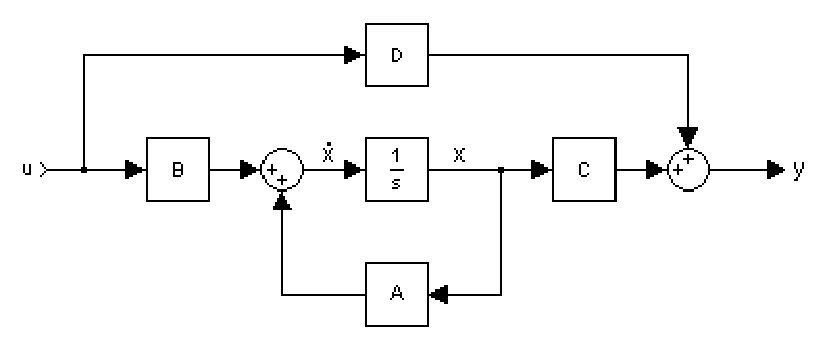
\includegraphics[width=250]{./figs/ssm.eps}
\end{figure}
\end{frame}

\begin{frame}{}
    \begin{itemize}
        \item Transfer Function from State Space model: $TF: H(s) = C[sI-A]^{-1}B + D = C\frac{Adj[sI-A]}{|sI-A|}B + D$
        \item $H(s) = \frac{\begin{bmatrix}
        1 & 0
        \end{bmatrix}\begin{bmatrix}
        s+3 & 1\\
        -2 & s
        \end{bmatrix}\begin{bmatrix}
        0\\
        1
        \end{bmatrix}}{s(s+3) + 2} = \LARGE{\frac{1}{s^{2}+3s+2}}$
        \item Therefore the poles of the transfer function are: s = -1 and s = -2
    \end{itemize}
\end{frame}



\begin{frame}{}
\begin{block}
\begin{itemize}
\item From first equation: $$\frac{\partial x_1(t)}{\partial t} =              x_2(t) $$
\item Substitution in second equation results into the equation:\vspace{5} $\frac{\partial^2 x_1}{\partial t^2} + 3\frac{\partial x_1(t)}{\partial t} + 2x_1(t) = r(t)$ 
\item Taking Laplace transform on both sides:\vspace{5}
$s^2X_1(s) + 3sX_1(s) + 2X_1(s) - sx_1(0) - x_1'(0) -3x_1(0)  = R(s)$
\item $ H(s) = \frac{X_1(s)}{R(s)} = \frac{1}{s^2 + 3s + 2}$
\item Therefore the poles of the transfer function are: s = -1 and s = -2
\end{itemize}
\end{block}

\end{frame}

\begin{frame}{}

\begin{itemize}
    \item Since the poles of the transfer function are real and distinct, the system is \textbf{OVERDAMPED}.
    \item Solution: $h(t) = L^{-1}(H(s)) = e^{-t} - e^{-2t}$
    \\\\\\
\end{itemize}

\end{frame}
\\\\\\
\begin{frame}{Question-28 }
The number of directions and encirclements around the point -1+j0 in the complex plane by the Nyquist plot of $$G(s) = \frac{1-s}{4+2s}$$

\bigskip
\begin{itemize}
    \item Zero
    \item One, Anti-Clock wise
    \item One, Clock wise
    \item Two, Clock wise
\end{itemize}
\end{frame}
\\\\
\begin{frame}{Solution:- }

First,we need to draw the polar plot of given G(S).
In the polar plot,substitute s = j\omega
\\
$$ G(j\omega) = \frac{1-j\omega}{4+2j\omega} $$
\\
$$ \lim_{\omega\to\infty} G(j\omega) = \frac{1-j\omega}{4+2j\omega} $$
\\
$$ \lim_{\omega\to\infty} G(j\omega) = \frac{j\omega(\frac{1}{j\omega}-1)}{j\omega(\frac{4}{j\omega}+2)} $$ 
\\
$$ \lim_{\omega\to\infty} G(j\omega) = \frac{-1}{2}\angle 0 $$ 
\\

\centering which is equal to $\frac{1}{2}\angle{-180}$
\end{frame}

\begin{frame}{}
As the Magnitude is taken positive in Nyquist Plot.\\
Now substitute \omega = 0
\\
$$ \lim_{\omega\to\ 0} G(j\omega) = \frac{1-j\omega}{4+2j\omega} = \frac{1}{4}\angle 0 $$

$$\angle Num(G(j\omega)) = \taninv \frac{-\omega}{1} = -\taninv \frac{\omega}{1}$$
\\
$$\angle Den(G(j\omega)) = \taninv \frac{\omega}{2} = \taninv \frac{\omega}{2}$$
\\
\angle $G(j\omega) = \angle Num(G(j\omega)) - \angle Den(G(j\omega))$

\bigskip
so from this  at $\omega = 0$ \angle $G(j\omega) = 0$

\bigskip
and so from this  at $\omega = $\infty$ \angle $G(j\omega)  =$-\pi$     
\end{frame}

\begin{frame}{}
$$ \mid(G(j\omega))\mid = \frac{\sqrt{1+{\omega}^2}}{\sqrt{16+{4\omega}^2}} $$
\\
when $\omega =0$ \mid(G(j\omega))\mid = \frac{1}{4}
\bigskip
\\

when $\omega = \infty$ $\mid(G(j\omega))\mid = \frac{1}{2}$
\bigskip
\\
Hence,magnitude should be every time positive.
\\
So,we have to plot first 0.25 then we have to turn {-180} degrees \\ to that point i.e {180} degrees clockwise(in this case)

\end{frame}
\begin{frame}{}
\begin{itemize}
\item Now Plot the Polar Plot 1 from $\omega$=0 to $\infty$
\\

$$ 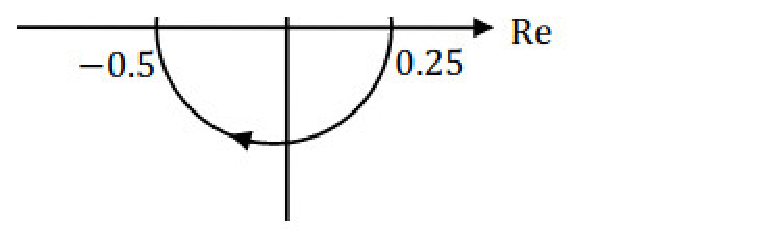
\includegraphics[scale = 0.5]{./figs/image2.eps}$$
\\
\item Draw the Mirror image of the Polar Plot 1.
\\
$$ 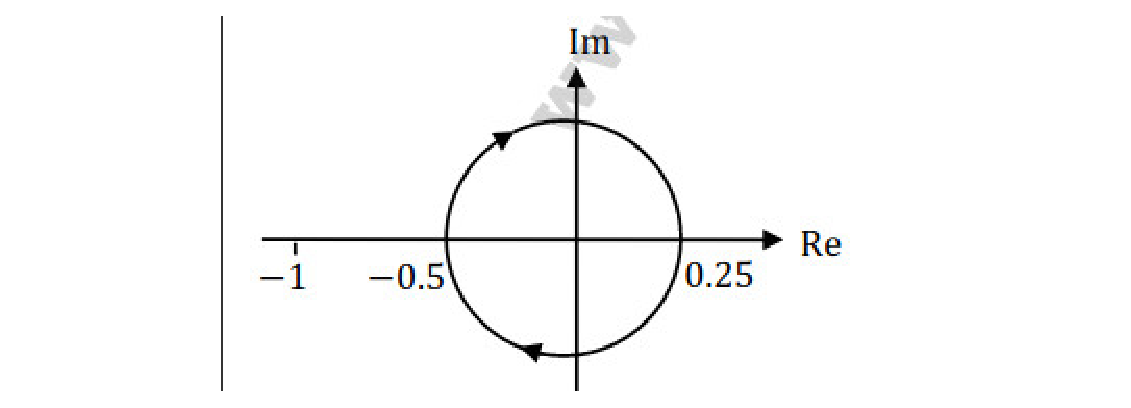
\includegraphics[scale = 0.5]{./figs/image1.eps}$$
\\
\item Find the points where $G(j\omega)$ intersects the real and imaginary axes(if needed) and then locate the given co-ordinate
\end{itemize}
\\
\bigskip

\end{frame}

\begin{frame}{}
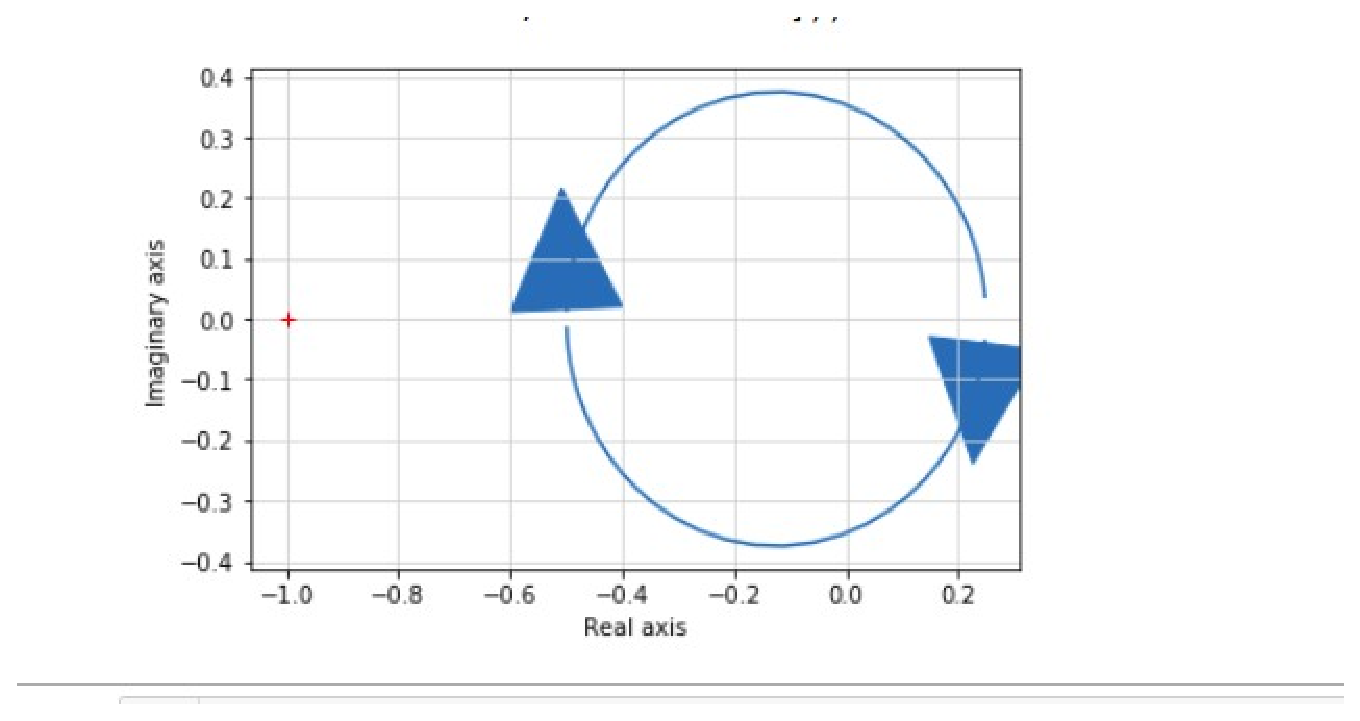
\includegraphics[scale = 0.5]{./figs/updated.eps}
\end{frame}

\begin{frame}{}
    $$Put\,s=Re^{j\theta}$$
    $$\lim_{R\to \infty}\,G(Re^{j\theta})=\frac{1-Re^{j\theta}}{4+2Re^{j\theta}}=\frac{-1}{2}$$ \\
    \bigskip
    As there are no $e^{j\theta}$ terms, 
    \\
    There there will be no enclosed Nyquist path here. 
    \\
    So, for this Transfer function $G(s)$,the Nyquist plot is same as the Polar plot.
    
\end{frame}

\begin{frame}{}
As from the observed plot the co-ordinate -1 + j0 is outside the contour
\\
\bigskip
\\
Hence,the number of encirclements around the the given co-ordinate is zero.
\end{frame}
\\
\\\\
\begin{frame}{Question-29 }
In the feedback system given below G(s)= \(\frac{1}{s^2+2s}\) .\\
The step response of the closed-loop system should have minimum settling time and have no overshoot.

\begin{figure}[h]
    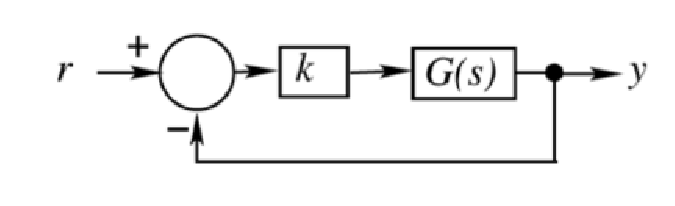
\includegraphics[scale=0.5]{./figs/fig-8.eps}
\end{figure}

The required value of gain k to achieve this is \underline{\hspace{2cm}}

\end{frame}

\begin{frame}{Solution:- }
$Settling Time$: The time required for the transient's damped oscillations to
reach and stay within ±2\% of the steady-state value.\vspace{5mm}


$Overshoot$:The amount that the waveform overshoots the steady state, or final, value at the peak time, expressed as a percentage of the steady-state
value.\\
\vspace{5mm}
The Transfer function of the negative unity feedback system is given by \(\frac{H(s)}{1+H(s)}\) (Where H(s) is the open-loop gain of the system) \\
\end{frame}
\begin{frame}{}
    

In the given Question H(s) = k x G(s).So, Transfer function of the whole feedback system is \(\frac{kG(s)}{1+kG(s)}\) \\
By Substituting G(s) function we get \(\frac{k}{s^2+2s+K}\)
\begin{figure}[h]
    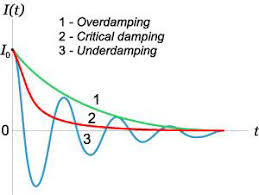
\includegraphics[scale=0.5]{./figs/fig-7.jpeg}

    
\end{figure}

By observing the above figure,minimum settling time is obtained for Critical Damped System.\\
\end{frame}

\begin{frame}{}
Also, Critically Damped System doesn't have overshoot.\\
Transfer function of the Critical Damped System is given by
\(\frac{\omega_n^2}{s^2+2\zeta\omega_ns +\omega_n^2}\) (Where, \zeta=1)\\
By comparing Obtained Transfer function \(\frac{k}{s^2+2s+K}\) and the general transfer function of Critical Damped System \(\frac{\omega_n^2}{s^2+2\zeta\omega_ns +\omega_n^2}\)\\
\vspace{5mm}\\
We get \zeta = \(\frac{1}{\sqrt{K}}\)\\
As \zeta = 1\\
\vspace{5mm}\\
\(\frac{1}{\sqrt{K}}\) =1\\
\vspace{5mm}\\
K=1\\
\vspace{5mm}\\
Therefore, The value of K is 1.\\




\end{frame}
\begin{frame}{}
\begin{figure}[h]
    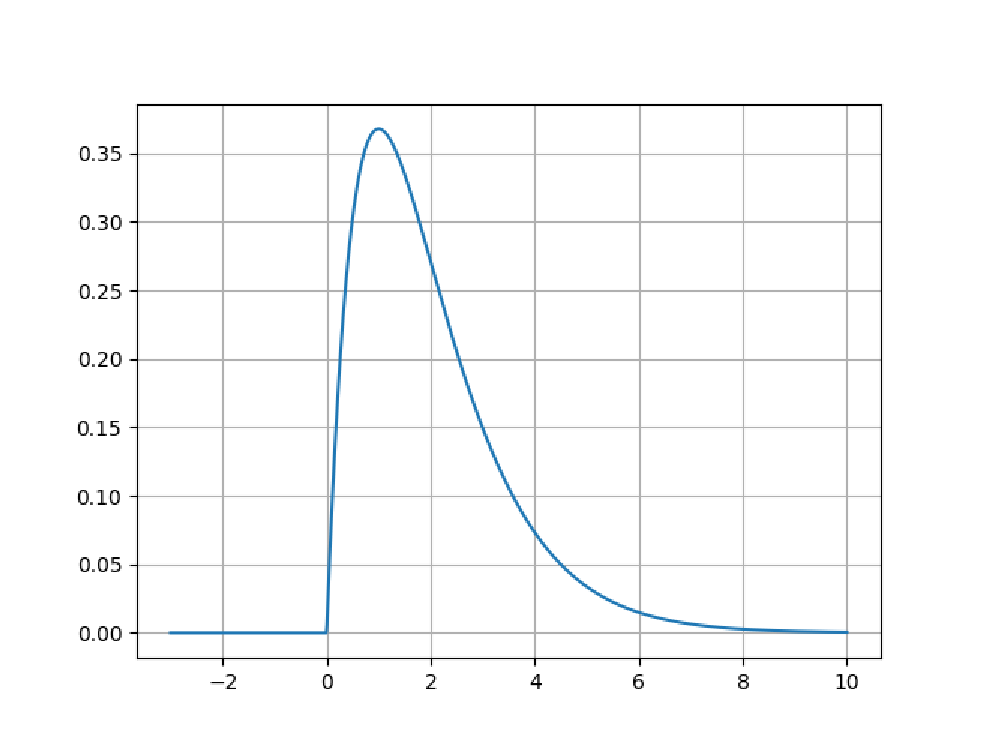
\includegraphics[scale=0.65]{./figs/fig-6.eps}
    
\end{figure}
\\\\
\\\\
\end{frame}
\\\\\\\\
\\\\\\\\\
\begin{frame}{Question-30 }
\begin{block}

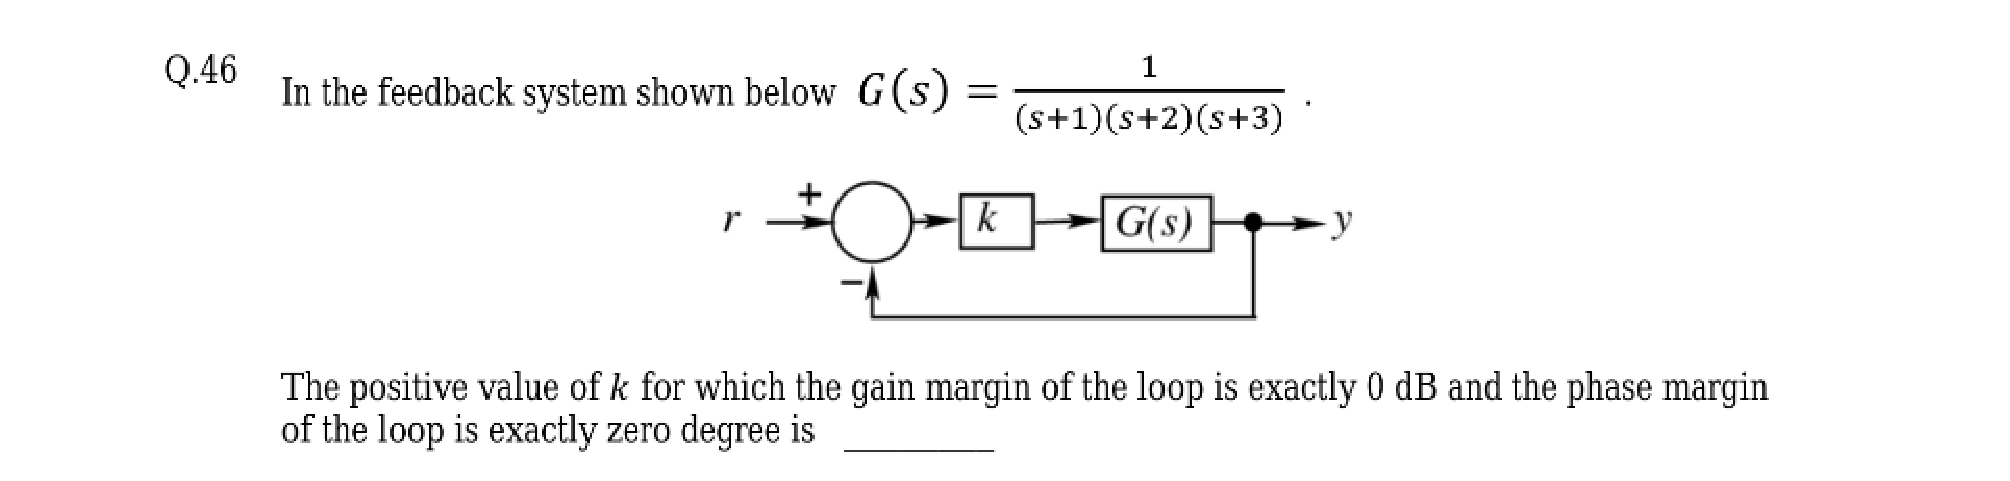
\includegraphics[scale=0.33]{./figs/1.eps}

\end{block}
\end{frame}
%\begin{frame}
%\tableofcontents
%\end{frame}

\begin{frame}{Solution:- }

\begin{block}

The gain margin is defined as the change in open-loop gain required to make the closed-loop system unstable. Systems with greater gain margins can withstand greater changes in system parameters before becoming unstable in closed-loop. 

\end{block} \vspace{16pt}
\begin{block}

The phase margin is defined as the change in open-loop phase shift required to make the closed-loop system unstable. The phase margin also measures the system's tolerance to time delay
\end{block} \vspace{16pt}




\end{frame}



\begin{frame}{}
\begin{block}

As given in question we see that gain margin is 0 dB and phase margin is 0 degrees. This implies that system is just enough stable and will become destabilized on just small increase in gain. Hence the system is marginbally stable.
\end{block}

\begin{block}

The stability of the system can be checked by Routh-Hurwitz Stability Criterion 
\end{block}

\end{frame}


\begin{frame}{}
\begin{block}
\\
Routh-Hurwitz Stability Criterion:- \\
Necessary condition for Routh-Hurwitz Stability Criterion: The necessary condition is that the coefficients of the characteristic polynomial should be positive. This implies that all the roots of the characteristic equation should have negative real parts.

Sufficient condition for Routh-Hurwitz Stability Criterion:The sufficient condition is that all the elements of the first column of the Routh array should have the same sign. This means that all the elements of the first column of the Routh array should be either positive or negative.\vspace{16pt}
\end{block}

\end{frame}

\begin{frame}{}
The Routh array for characteristic equation $a_0s^n+a_1s^{n-1}+a_2s^{n-2}+a_3s^{n-3}.....+a_n$
\begin{table}[]
\begin{tabular}{lllll}
$s^n$ & $a_0$ & $a_2$ &  &  \\
$s^(n-1)$ & $a_1$ & $a_3$ &  &  \\
$s^(n-2)$ & 2 & 0 &  &  \\
$s^(n-3)$ & 0 & 0 &  & 
\end{tabular}
\end{table}
\end{frame}

\begin{frame}{}
The Routh array for equation $s^3+6s^2+11s^1+(6+k)$
\begin{table}[]
\begin{tabular}{lllll}
$s^3$ & 1            & 11    &  &  \\
$s^2$ & 6            & (6+k) &  &  \\
$s^1$ & $\frac{66-(6+K)}{6}$& 0     &  &  \\
$s^0$ & $(6+k)$        & 0     &  & 


\end{tabular}
\end{table}
Now since the system is marginally stable therefore $s^1$ row is $\geq$ 0\newline
Hence $\frac{66-(6+K)}{6}\geq$ 0
Hence k=60
\end{frame}



\end{enumerate}
\end{document}


